\documentclass{article}
\usepackage[utf8]{inputenc}
\usepackage{hyperref}

\usepackage[english]{babel}
\usepackage{latexsym,bm,amsmath,amssymb,graphicx,ctex,tikz,systeme,array, soul,scalerel,wrapfig,lipsum, float}
\newcommand*\circled[1]{\tikz[baseline=(char.base)]{
            \node[shape=circle,draw,inner sep=2pt] (char) {#1};}}
\usepackage{extarrows}% http://ctan.org/pkg/extarrows
\newcommand*{\vertbar}{\rule[-1ex]{0.5pt}{2.5ex}}
\newcommand*{\horzbar}{\rule[.5ex]{2.5ex}{0.5pt}}
\newcommand{\eqdef}{\xlongequal{\text{def}}}%
\usepackage{geometry}
 \geometry{
 a4paper,
 total={170mm,257mm},
 left=10mm,
 right=10mm,
 top=20mm,
 }
\usepackage{subfig}
\usepackage{wrapfig}
\usepackage{multirow}
\usepackage{multicol}
\usepackage{graphicx}
\usepackage{titling}
\usepackage{listings}
\usepackage{xcolor}
\usepackage[lighttt]{lmodern}
\definecolor{codegreen}{rgb}{0,0.6,0}
\definecolor{codegray}{rgb}{0.2,0.2,0.2}
\definecolor{codepurple}{rgb}{0.58,0,0.82}
\definecolor{keyblue}{rgb}{0,0,0.9}
\definecolor{backcolour}{rgb}{0.98,0.98,0.98}
\lstdefinestyle{mystyle}{
    backgroundcolor=\color{backcolour},   
    commentstyle=\color{codepurple},
    keywordstyle=\color{keyblue},
    numberstyle=\tiny\color{codegray},
    stringstyle=\color{codepurple},
    basicstyle=\ttfamily\small,
    breakatwhitespace=false,         
    breaklines=true,                 
    captionpos=t,                    
    keepspaces=true,                 
    numbers=left,                    
    numbersep=1pt,                  
    showspaces=false,                
    showstringspaces=false,
    showtabs=false,                  
    tabsize=1
}
% -- Setting up the custom style:
\lstset{style=mystyle}
% ======= code block =======
\usepackage{xcolor} % 必须加载

% 定义灰色背景颜色
\definecolor{graybg}{RGB}{240,240,240}

% ==========================

\lstset{style=mystyle}
\newcommand{\subs}[1]{\subsection*{#1}}
\newcommand{\secs}[1]{\section*{#1}}
 
\usepackage{fancyhdr}
\fancypagestyle{plain}{%  the preset of fancyhdr 
    \fancyhf{} % clear all header and footer fields
    \fancyfoot[R]{Guyuan Xu\\224040074}
    \fancyfoot[L]{\thedate}
    \fancyhead[L]{MDS 5122 Deep Learning and Application}
    % \fancyhead[R]{\theauthor}
}
\makeatletter
\def\@maketitle{%
  \newpage
  \null
  \vskip 1em%
  \begin{center}%
  \let \footnote \thanks
    {\LARGE \@title \par}%
    \vskip 1em%
    %{\large \@date}%
  \end{center}%
  \par
  \vskip 1em}
\makeatother

% \usepackage{lipsum}  
% \usepackage{cmbright}



%======================================= document ======================================
%======================================= document ======================================
%======================================= document ======================================

\begin{document}
\title{\raggedright MDS 5122 Assignment 1}
%\author{Guyuan Xu \\224040074}
\date{March 9, 2025}
\maketitle

\noindent\begin{tabular}{@{}ll}
   Guyuan Xu &\href{mailto:224040074@link.cuhk.edu.cn}{224040074} \\
    
%
\end{tabular}

\secs{A. Build a Neural Network Using PyTorch}
\subs{1. reproducing example NeuralNetwork of example code A.}
\textcolor{blue}{Results are summaried in subsection 2.2 together with other settings, codes check notebook}

\subs{2. Factors to improve accuracy}
In my experiment, I tried to use 1) Simple NN structure(which is the baseline model of example code A) and NN with more complex architecture (vgg16 and ResNet18/50); 2) adding BatchNorm layer and dropout layer; 3) different optimziers SGD and Adam with popular \textit{lr} or momentum params settings; 4) with/without data augmentation. \\

We mainly use the model of example code-A as our baseline model to examine how the above factors might affect accuracy. And due to computing resource limitation, i did not conduct strict experiment with strict variable controls. To gain insight is what we want.\\


% \noindent\textbf{- BaseLine Model }: C3L3 (3 Conv layers + 3 Linear layers) on CIFAR-10 dataset\\
% We first start with baseline model in example-code A, the steps of experiment are: 1)compare optimziers with all other settings the same, then pick the best optimziers (in terms of accuracy) for next step; 2) use the best optimizer and data augmentation to see if data augmentation could bring up accuracy in test set; 3) use best optimizer + data augmentation(note that data augmentation might not be useful, shall be given up if so) + \textcolor{red}{BatchNorm Layer} + \textcolor{red}{throw away dropout layer in convolution layer} to see whether we can have better accuracy on test set. 

% \noindent\textbf{Experiments Setup}\\
\subs{2.0 Experiments Setup: How to run}
All training codes are packed in files located in \texttt{./kaggleFile}, what are those \texttt{.ipynb} files' names mean:
\begin{itemize}
  \item All files start with \texttt{main\_} are training files
  \item if not specify explicitly in file name, models are trained in CIFAR-10 dataset.
  \item \texttt{main\_bsln\_4} means "baseline model" with setting number 4 on CIFAR-10, \texttt{main\_res18} means "ResNet18" model on CIFAR-10 
  \item change "code\_file" in \texttt{./kaggleFile/kernel-metadata.json} to the file name you want to run. Then push it to kaggle. \textcolor{red}{All training results/weights, including visualization of train/test loss and test accuracy will be saved to /kaggle/output automatically.}
\end{itemize}

\noindent \textbf{2.1 Baseline Convolutional Neural Network (C5L3) }
\begin{itemize}
  \item   architecture:  5 conv layers, each followed by a dropout layer (rate=0.3); 3 linear layers, each followed by a dropout layer (rate=0.5).
  \item   optimizer: Adam with a learning rate of 3e-4 and weight decay of 1e-6.
  \item   dataset: Trained on the CIFAR-10 dataset. The training set has dimensions (60,000, 3, 32, 32), and the test set has dimensions (10,000, 3, 32, 32).
  \item   Training settings: Trained for 150 epochs with a batch size of 64. Model accuracy was evaluated on the test set.
\end{itemize}
\vspace{5mm}
\noindent \textbf{2.2 C5L3 architecture and data prep overview}
% \begin{verbatim}
% # baseline model(C5L3) architecture:  
%   net = nn.Sequential(
%       nn.Conv2d(3, 128, 3, padding=1), nn.ReLU(inplace=True), nn.MaxPool2d(2), nn.Dropout(0.3),
%       nn.Conv2d(128, 256, 3, padding=1), nn.ReLU(inplace=True), nn.MaxPool2d(2), nn.Dropout(0.3),
%       nn.Conv2d(256, 512, 3, padding=1), nn.ReLU(inplace=True),
%       nn.Conv2d(512, 512, 3, padding=1), nn.ReLU(inplace=True),
%       nn.Conv2d(512, 256, 3, padding=1), nn.ReLU(inplace=True), nn.MaxPool2d(2), nn.Dropout(0.3),
%       nn.Flatten(),

%       nn.Linear(256 * 4 * 4, 512), nn.ReLU(inplace=True), nn.Dropout(0.5),
%       nn.Linear(512, 256), nn.ReLU(inplace=True), nn.Dropout(0.5),
%       nn.Linear(256, 128), nn.ReLU(inplace=True), nn.Dropout(0.5),
%       nn.Linear(128, 10),
%   )
% # Params count: 3*128*3*3+128*256*3*3+256*512*3*2*3+512**2*3*3+256*16*512+512*256+256*128+1280=7.28M

% # Using default data transformation in example code-A
%   transformation = dict()
%   for data_type in ("train", "test"):
%     is_train = data_type=="train"
%     transformation[data_type] = tv_transforms.Compose((
%       [
%       # default data augmenation
%         tv_transforms.RandomRotation(degrees=15),
%         tv_transforms.RandomHorizontalFlip(),
%         tv_transforms.RandomAffine(degrees=0, translate=(0.1, 0.1)),
      
%       # extra data augmentation:
%         tv_transforms.ColorJitter(
%           brightness=0.2, 
%           contrast=0.2,
%           saturation=0.2,
%           hue=0.1)
%       ] if is_train else []) + 
%     [
%         tv_transforms.ToTensor(),
%         tv_transforms.Normalize(mean=[0.5, 0.5, 0.5], std=[0.5, 0.5, 0.5]),
%     ])
%   \end{verbatim}

\begin{lstlisting}[language=python]
  # baseline model(C5L3) architecture:  
  net = nn.Sequential(
    # conv layer: 5
      nn.Conv2d(3, 128, 3, padding=1), nn.ReLU(inplace=True), nn.MaxPool2d(2), nn.Dropout(0.3),
      nn.Conv2d(128, 256, 3, padding=1), nn.ReLU(inplace=True), nn.MaxPool2d(2), nn.Dropout(0.3),
      nn.Conv2d(256, 512, 3, padding=1), nn.ReLU(inplace=True),
      nn.Conv2d(512, 512, 3, padding=1), nn.ReLU(inplace=True),
      nn.Conv2d(512, 256, 3, padding=1), nn.ReLU(inplace=True), nn.MaxPool2d(2), nn.Dropout(0.3),
      nn.Flatten(),

    # linear layer: 3, excluding the last layer
      nn.Linear(256 * 4 * 4, 512), nn.ReLU(inplace=True), nn.Dropout(0.5),
      nn.Linear(512, 256), nn.ReLU(inplace=True), nn.Dropout(0.5),
      nn.Linear(256, 128), nn.ReLU(inplace=True), nn.Dropout(0.5),
      nn.Linear(128, 10),
  )
# ParamsCount: 3*128*3*3+128*256*3*3+256*512*3*2*3+512**2*3*3+256*16*512+512*256+256*128+1280=7.28M

# Using default data transformation in example code-A
  transformation = dict()
  for data_type in ("train", "test"):
    is_train = data_type=="train"
    transformation[data_type] = tv_transforms.Compose((
      [
      # default data augmenation
        tv_transforms.RandomRotation(degrees=15),
        tv_transforms.RandomHorizontalFlip(),
        tv_transforms.RandomAffine(degrees=0, translate=(0.1, 0.1)),
      
      # extra data augmentation:
        tv_transforms.ColorJitter(
          brightness=0.2, 
          contrast=0.2,
          saturation=0.2,
          hue=0.1)
      ] if is_train else []) + 
    [
        tv_transforms.ToTensor(),
        tv_transforms.Normalize(mean=[0.5, 0.5, 0.5], std=[0.5, 0.5, 0.5]),
    ])
\end{lstlisting}





\noindent Example of data augmentation on CIFAR-10:

% \begin{center}
%   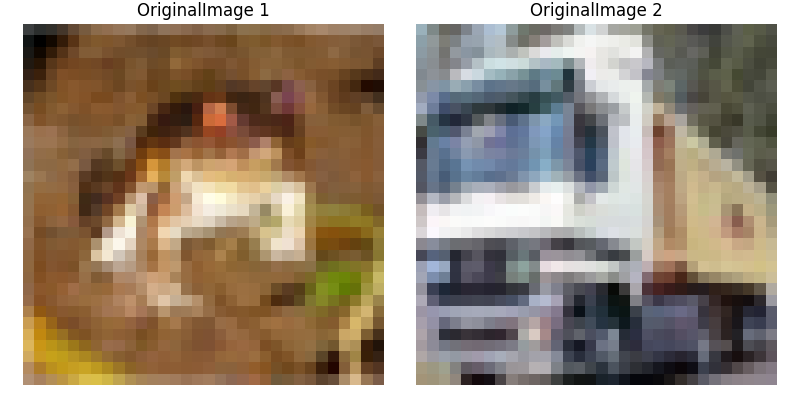
\includegraphics[width=0.45\textwidth]{fig/original.png} % 设定图片宽度为文本宽度的80%
%   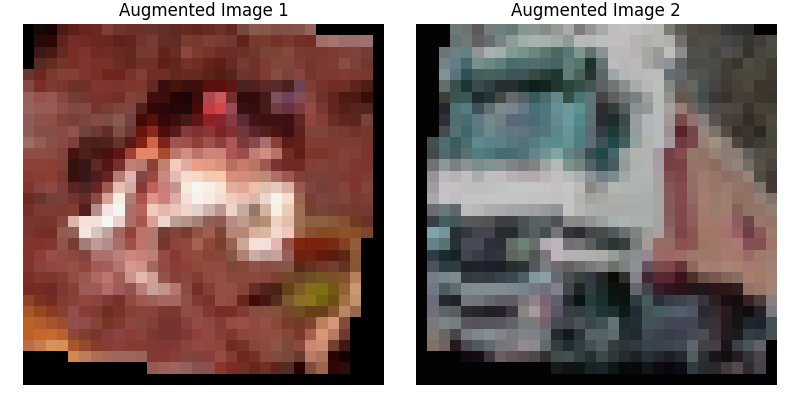
\includegraphics[width=0.45\textwidth]{fig/augmented.png} % 设定图片宽度为文本宽度的80%
% \end{center}
% \begin{center}
%   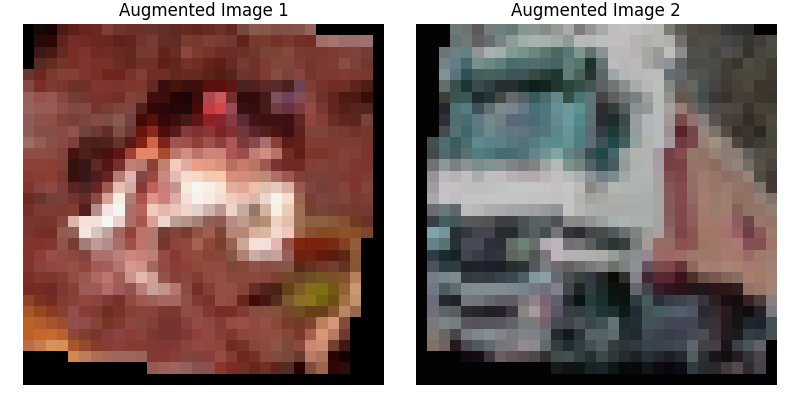
\includegraphics[width=0.8\textwidth]{fig/augmented.png} % 设定图片宽度为文本宽度的80%
% \end{center}
\begin{figure}[htbp]
  \centering
  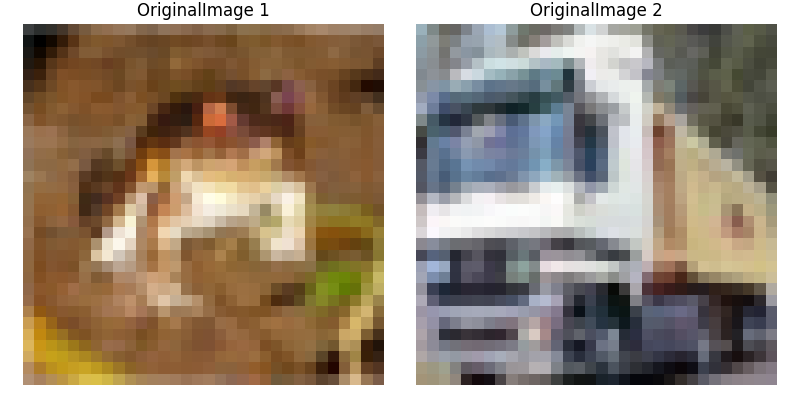
\includegraphics[width=0.45\textwidth]{fig/original.png} % 设定图片宽度
  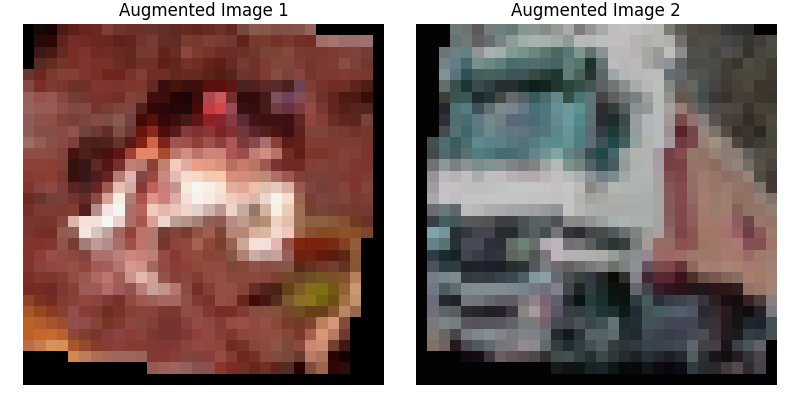
\includegraphics[width=0.45\textwidth]{fig/augmented.png} % 设定图片宽度
  \caption{original(left), augmented(right):random filp/rotate/affine/colorjit } % 图片标题
  \label{fig:original} % 图片标签,方便引用
\end{figure}

\noindent\textbf{Training strategies}
We have 6 (basline models with different settings on CIFAR-10) + 3 (advanced network on CIFAR-10) + 1 (best model on MNIST) = 10 models in total to train. We decided to run 10 separates .ipynb on kaggle, 1 for each model with it's corresponding settings, insteading of packing all in one file for the following reasons:

\begin{itemize}
  \item Parallel: kaggle allows running 2 notebook at the same time, save time.
  \item Flexibility: we can adjust each model at any time.
  \item Fault tolerance: If we run everything in 1 file, we will loose everything if 1 error pop up, wasting time quota of free gpu usage.
\end{itemize}



\noindent\textbf{2.2 Baseline model + additional modifications beyond the Baseline(C5L3):}
\begin{itemize}
  \item Extra Data Augmentation: Aside from default techniques in baselline model including random flipping, random rotation, random affine transformation, we add random brightness adjustments, and saturation modifications.
  \item Optimizer Variant: Replaced Adam with SGD (learning rate=1e-3).
  \item Architectural Varaint: Removed dropout layers after convolutional layers (retained dropout for linear layers), or adding BatchNorm layers after convolutional layers.
\end{itemize}


% ========= describe exp setting =========
\noindent Results on \textcolor{red}{CIFAR-10} are summarized in the folloing table

\begin{table}[htbp]
  \centering
  \caption{ModelSettings and Performance}
  \label{tab:model-compare}
  \begin{tabular}{|c|c|ccccc|} 
    \hline
    Model &\textcolor{red}{C5L3 base} &  &  & C5L3 variant & &   \\
    \hline
    SettingNo. &1 &2  &\textcolor{blue}{3}  & 4 &5 &6   \\
    \hline
    Adam &  \textcolor{red}{ $\surd$ }   &  & \textcolor{blue}{$\surd$} & $\surd$ & $\surd$  & $\surd$\\ 
    SGD & & $\surd$   & & &  &\\
    ExtraDataAug& &  & \textcolor{blue}{$\surd$} &  $\surd$ &  &$\surd$\\
    dropout &\textcolor{red}{all} & all   & \textcolor{blue}{linear}& none & linear  & linear \\ 
    BatchNorm & & & \textcolor{blue}{conv} & conv  & conv & conv \\ 
    MaxEpoch & \textcolor{red}{150} & 150 & \textcolor{blue}{150} & 150  & 150 & 256 \\
    \hline
    BestTestAccu & \textcolor{red}{85.11} &84.95 &\textcolor{blue}{89.31} & 89.69& 88.34 & 89.73 \\
    BestEpoch & 134 &146    &118 & 147 & 84  & 236\\
    \hline
  \end{tabular} 
\end{table}
\vspace{5mm}
\noindent We now interprate the results together with the curve of train/test loss + test accuracy.\\

\noindent 1) Figure 2 shows the train/test results of training setting 1 and 2: same on model structure + no data aug + full dropout after all layer, only differ in optimizer, where setting 1 adopt Adam and setting 2 adopt SGD. It is obvious that Adam covnerge faster than SGD, while the best testing accuray is almost the same: ~85\%. And we can also find that Adam one might be over fitted: for the testing loss(tagged validation loss, although this is not validation techinically) goes up after epoch ~40, while SGD's testing loss descent steadily.\\
\begin{figure}[H]
  \centering
  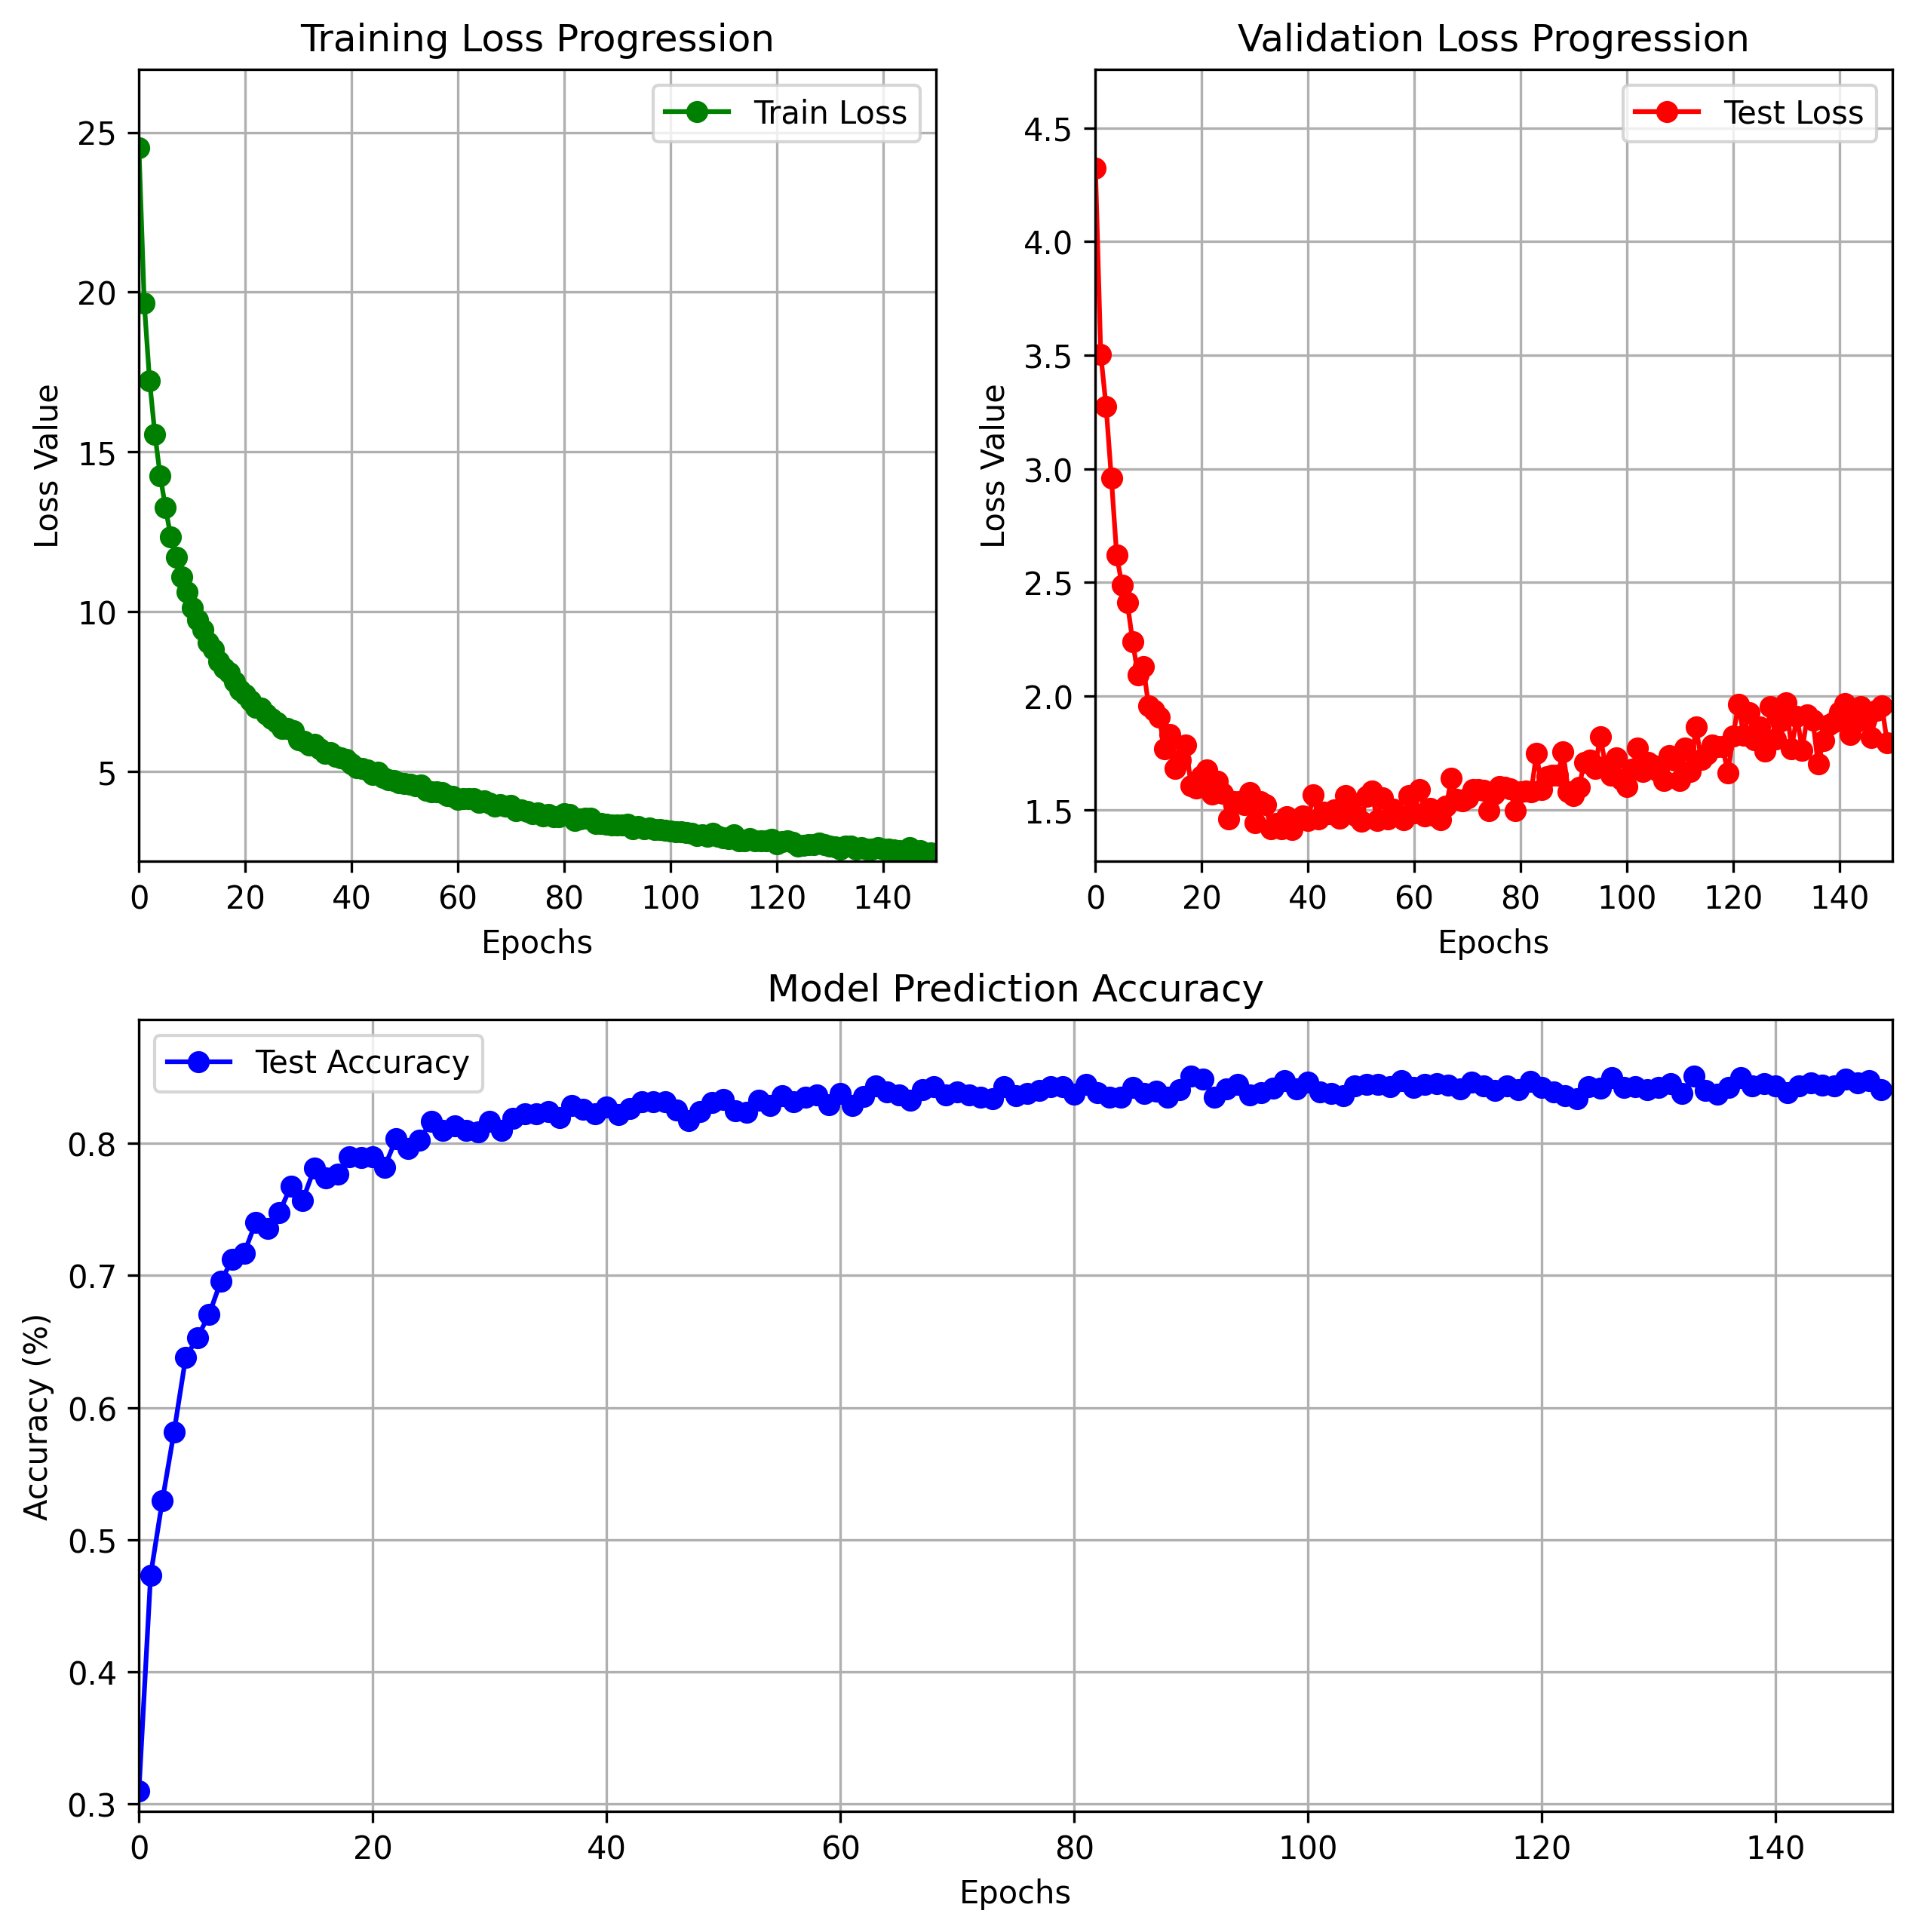
\includegraphics[width=0.35\textwidth]{fig/train_result_1.png} % 设定图片宽度
  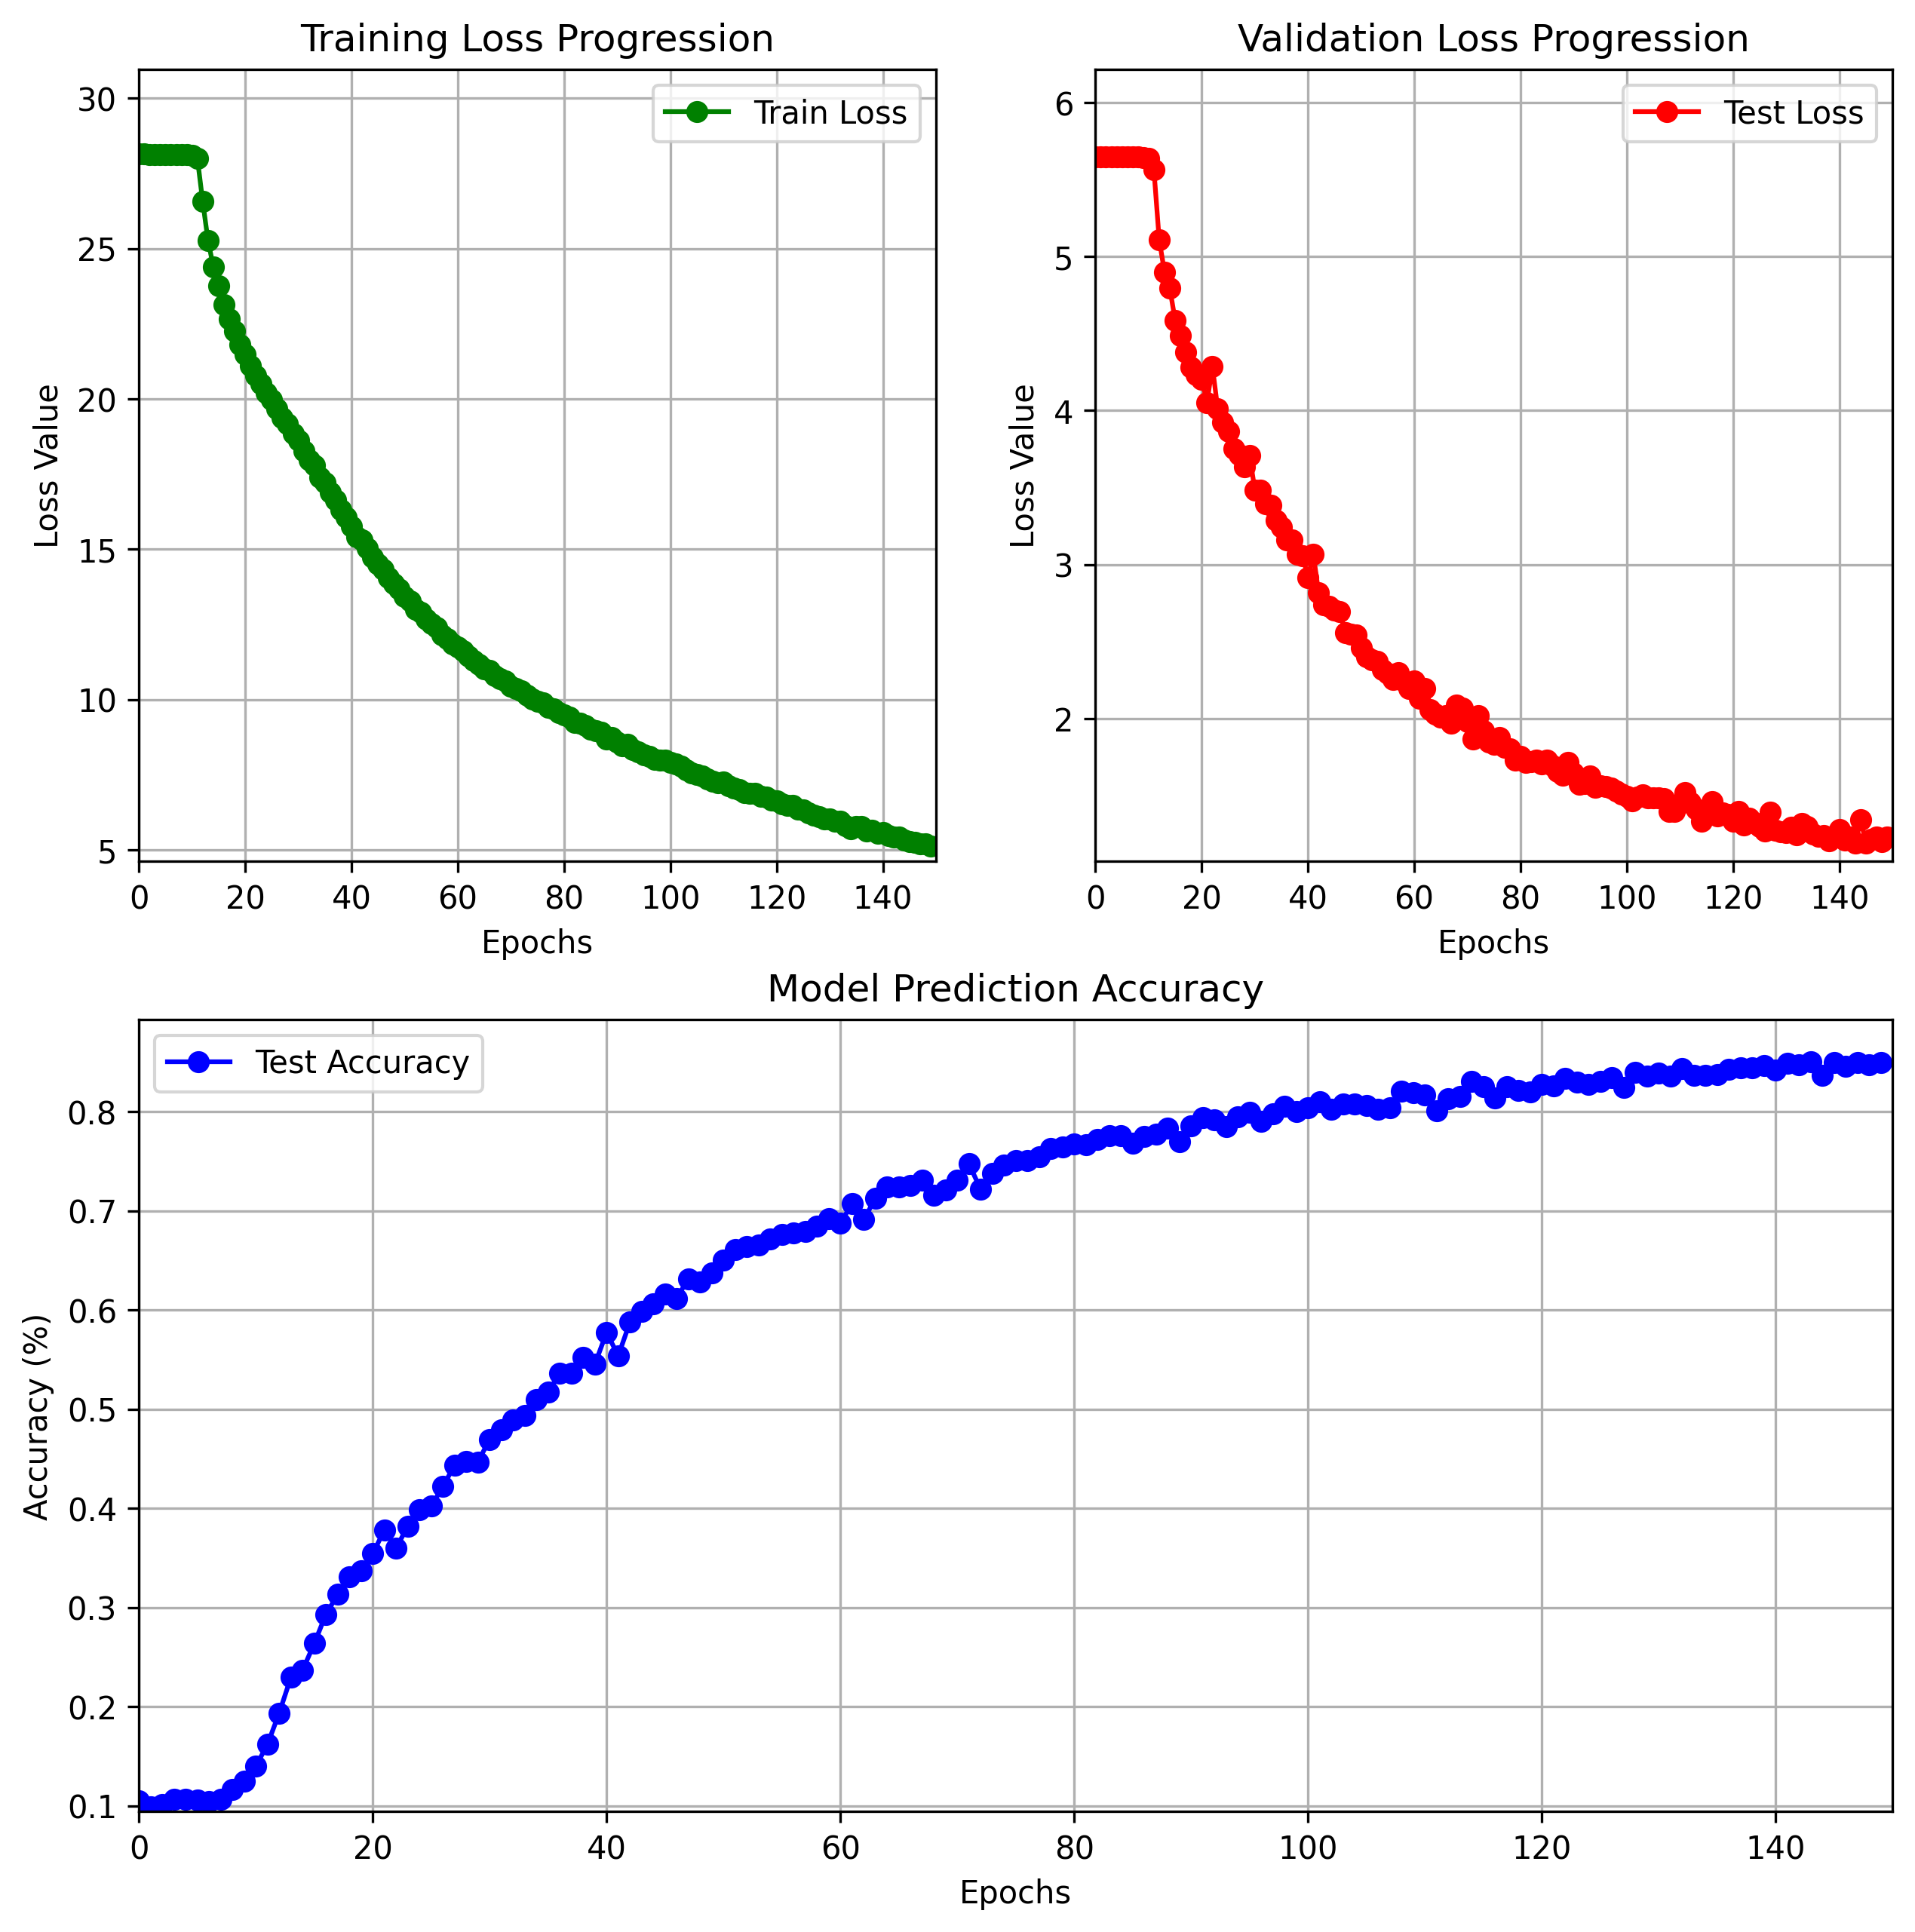
\includegraphics[width=0.35\textwidth]{fig/train_result_2.png} % 设定图片宽度
  \caption{model settings 1(left):Adam 2(right):SGD} % 图片标题
  \label{fig:curve} % 图片标签,方便引用
\end{figure}

\noindent 2) Figure 3 shows setting 3 and 3: same on model structure and other, only differ in whether using extra data augmentation (Color jitter), seems data augmentation is usefull cause the test accuracy is higher by 1\%, and they have almost the same curves.\\

\begin{figure}[hbtp]
  \centering
  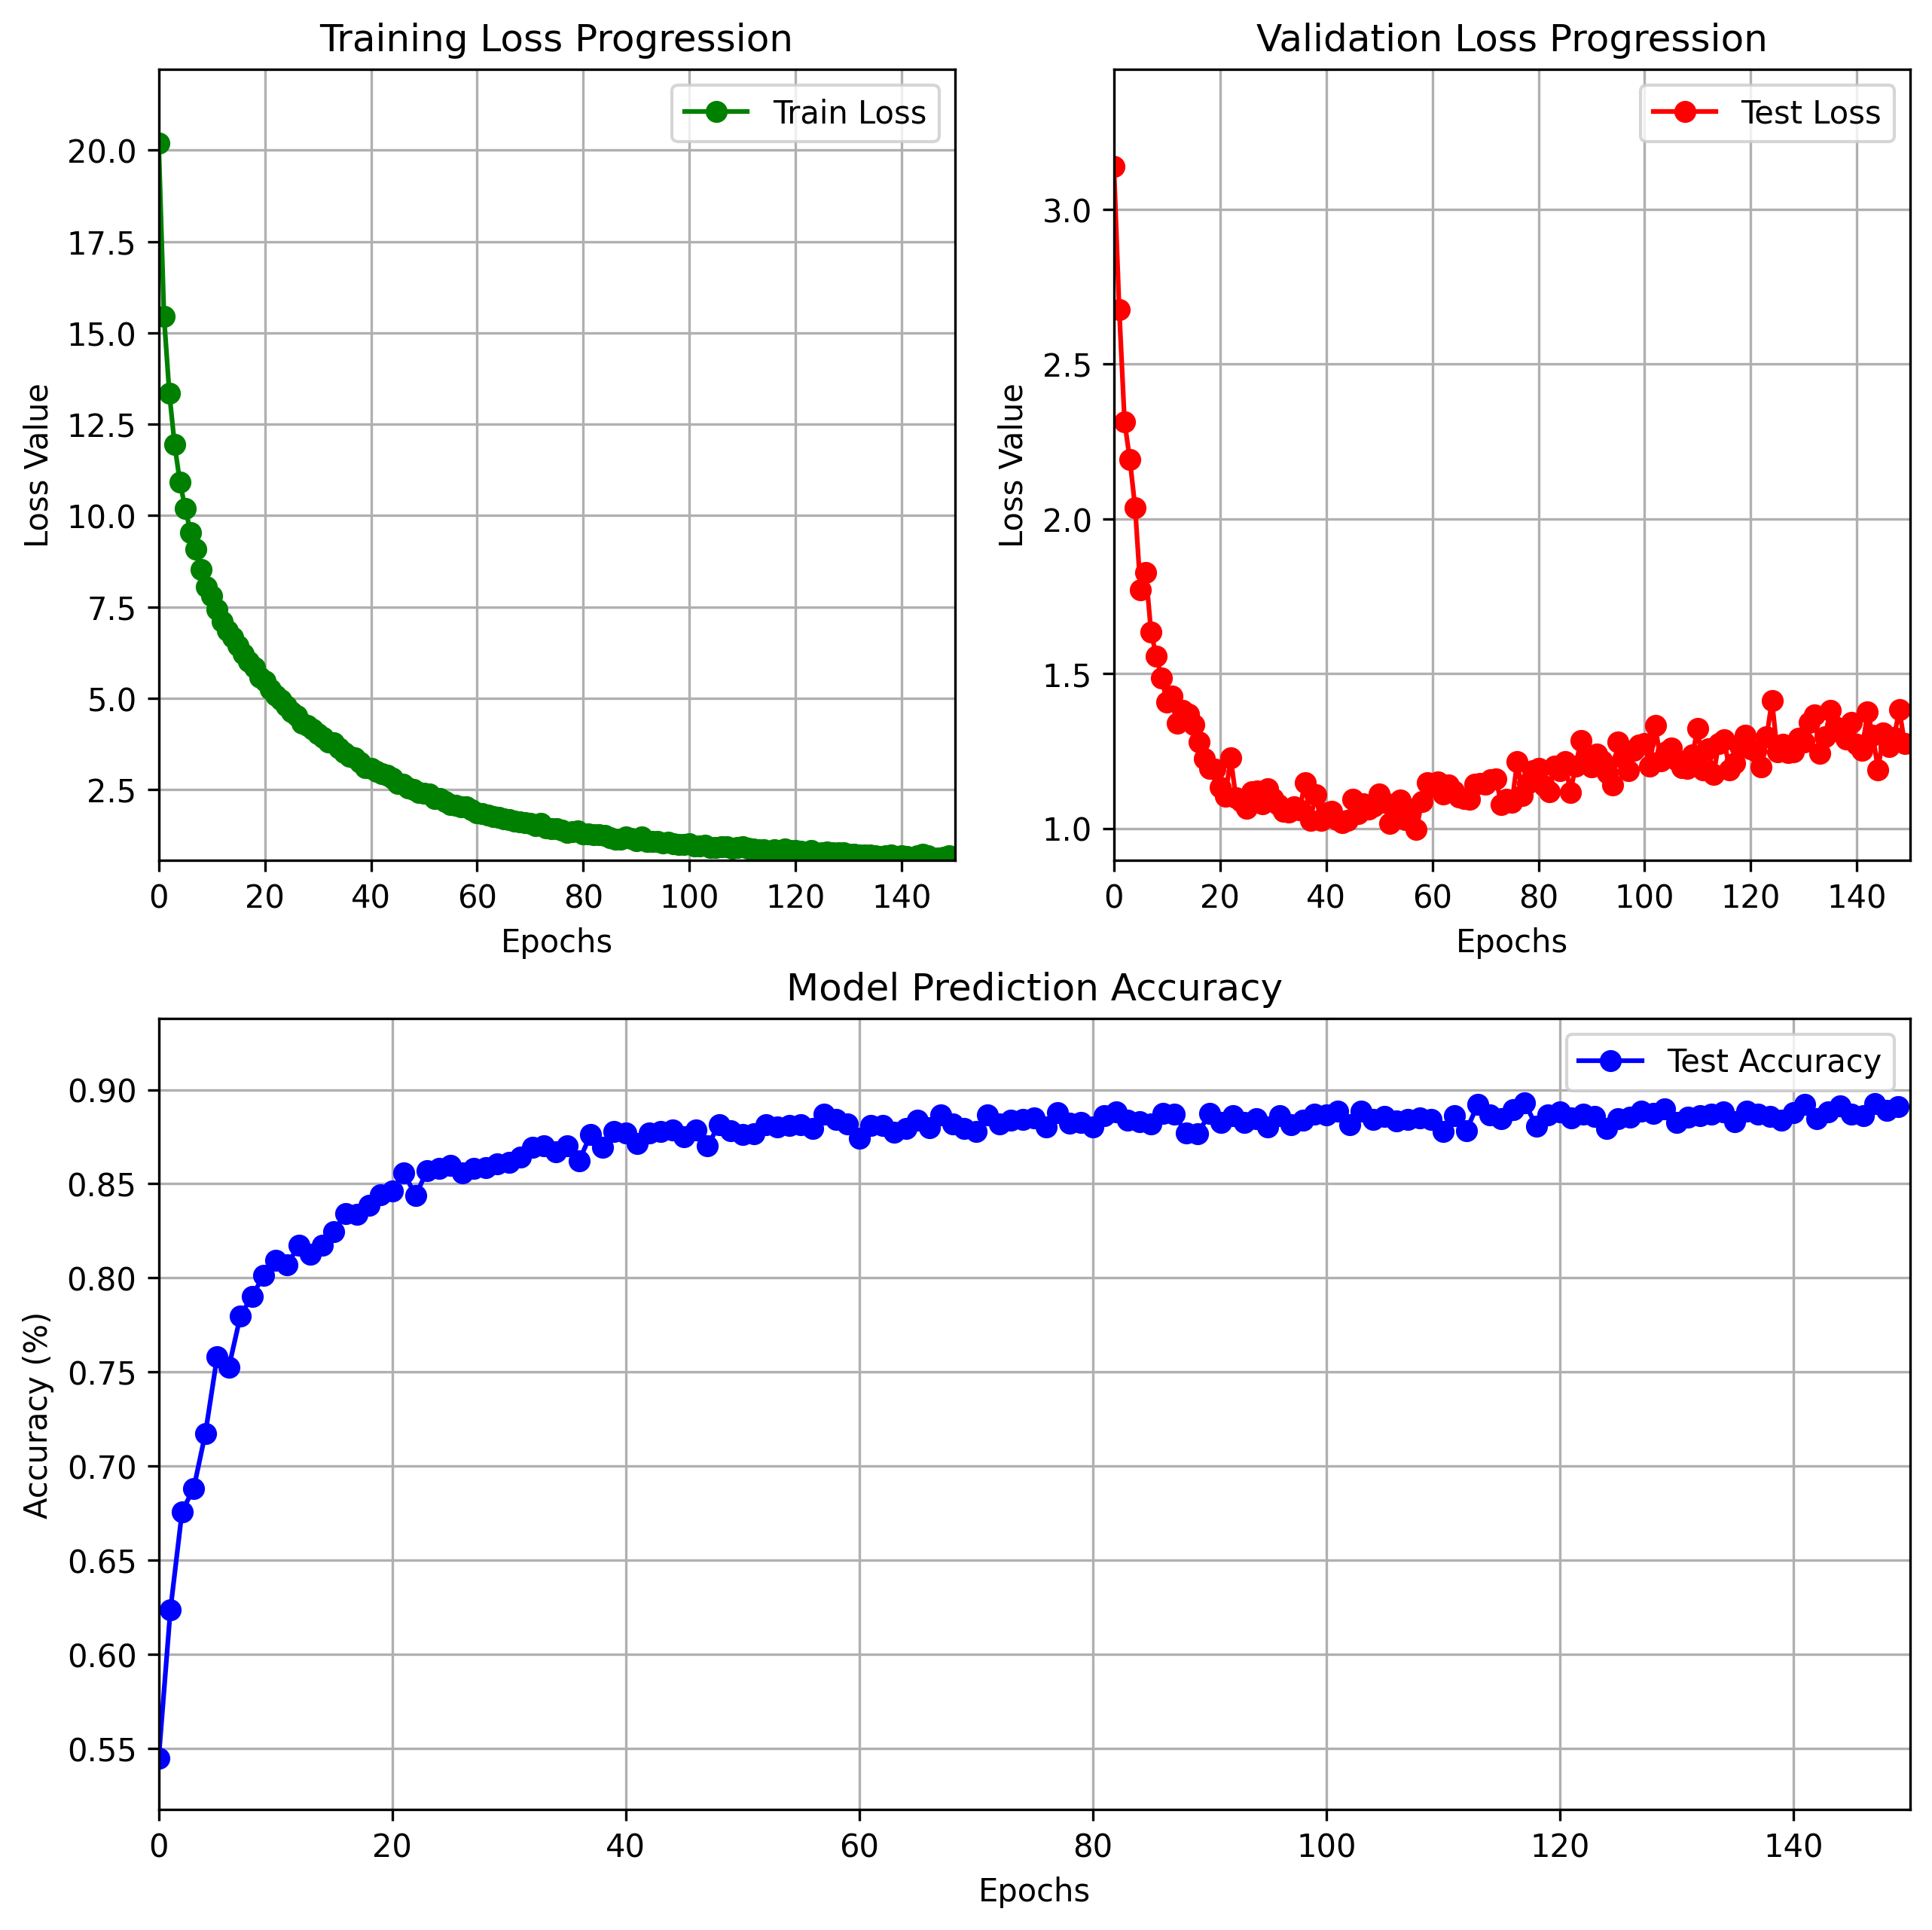
\includegraphics[width=0.45\textwidth]{fig/train_result_3.png} % 设定图片宽度
  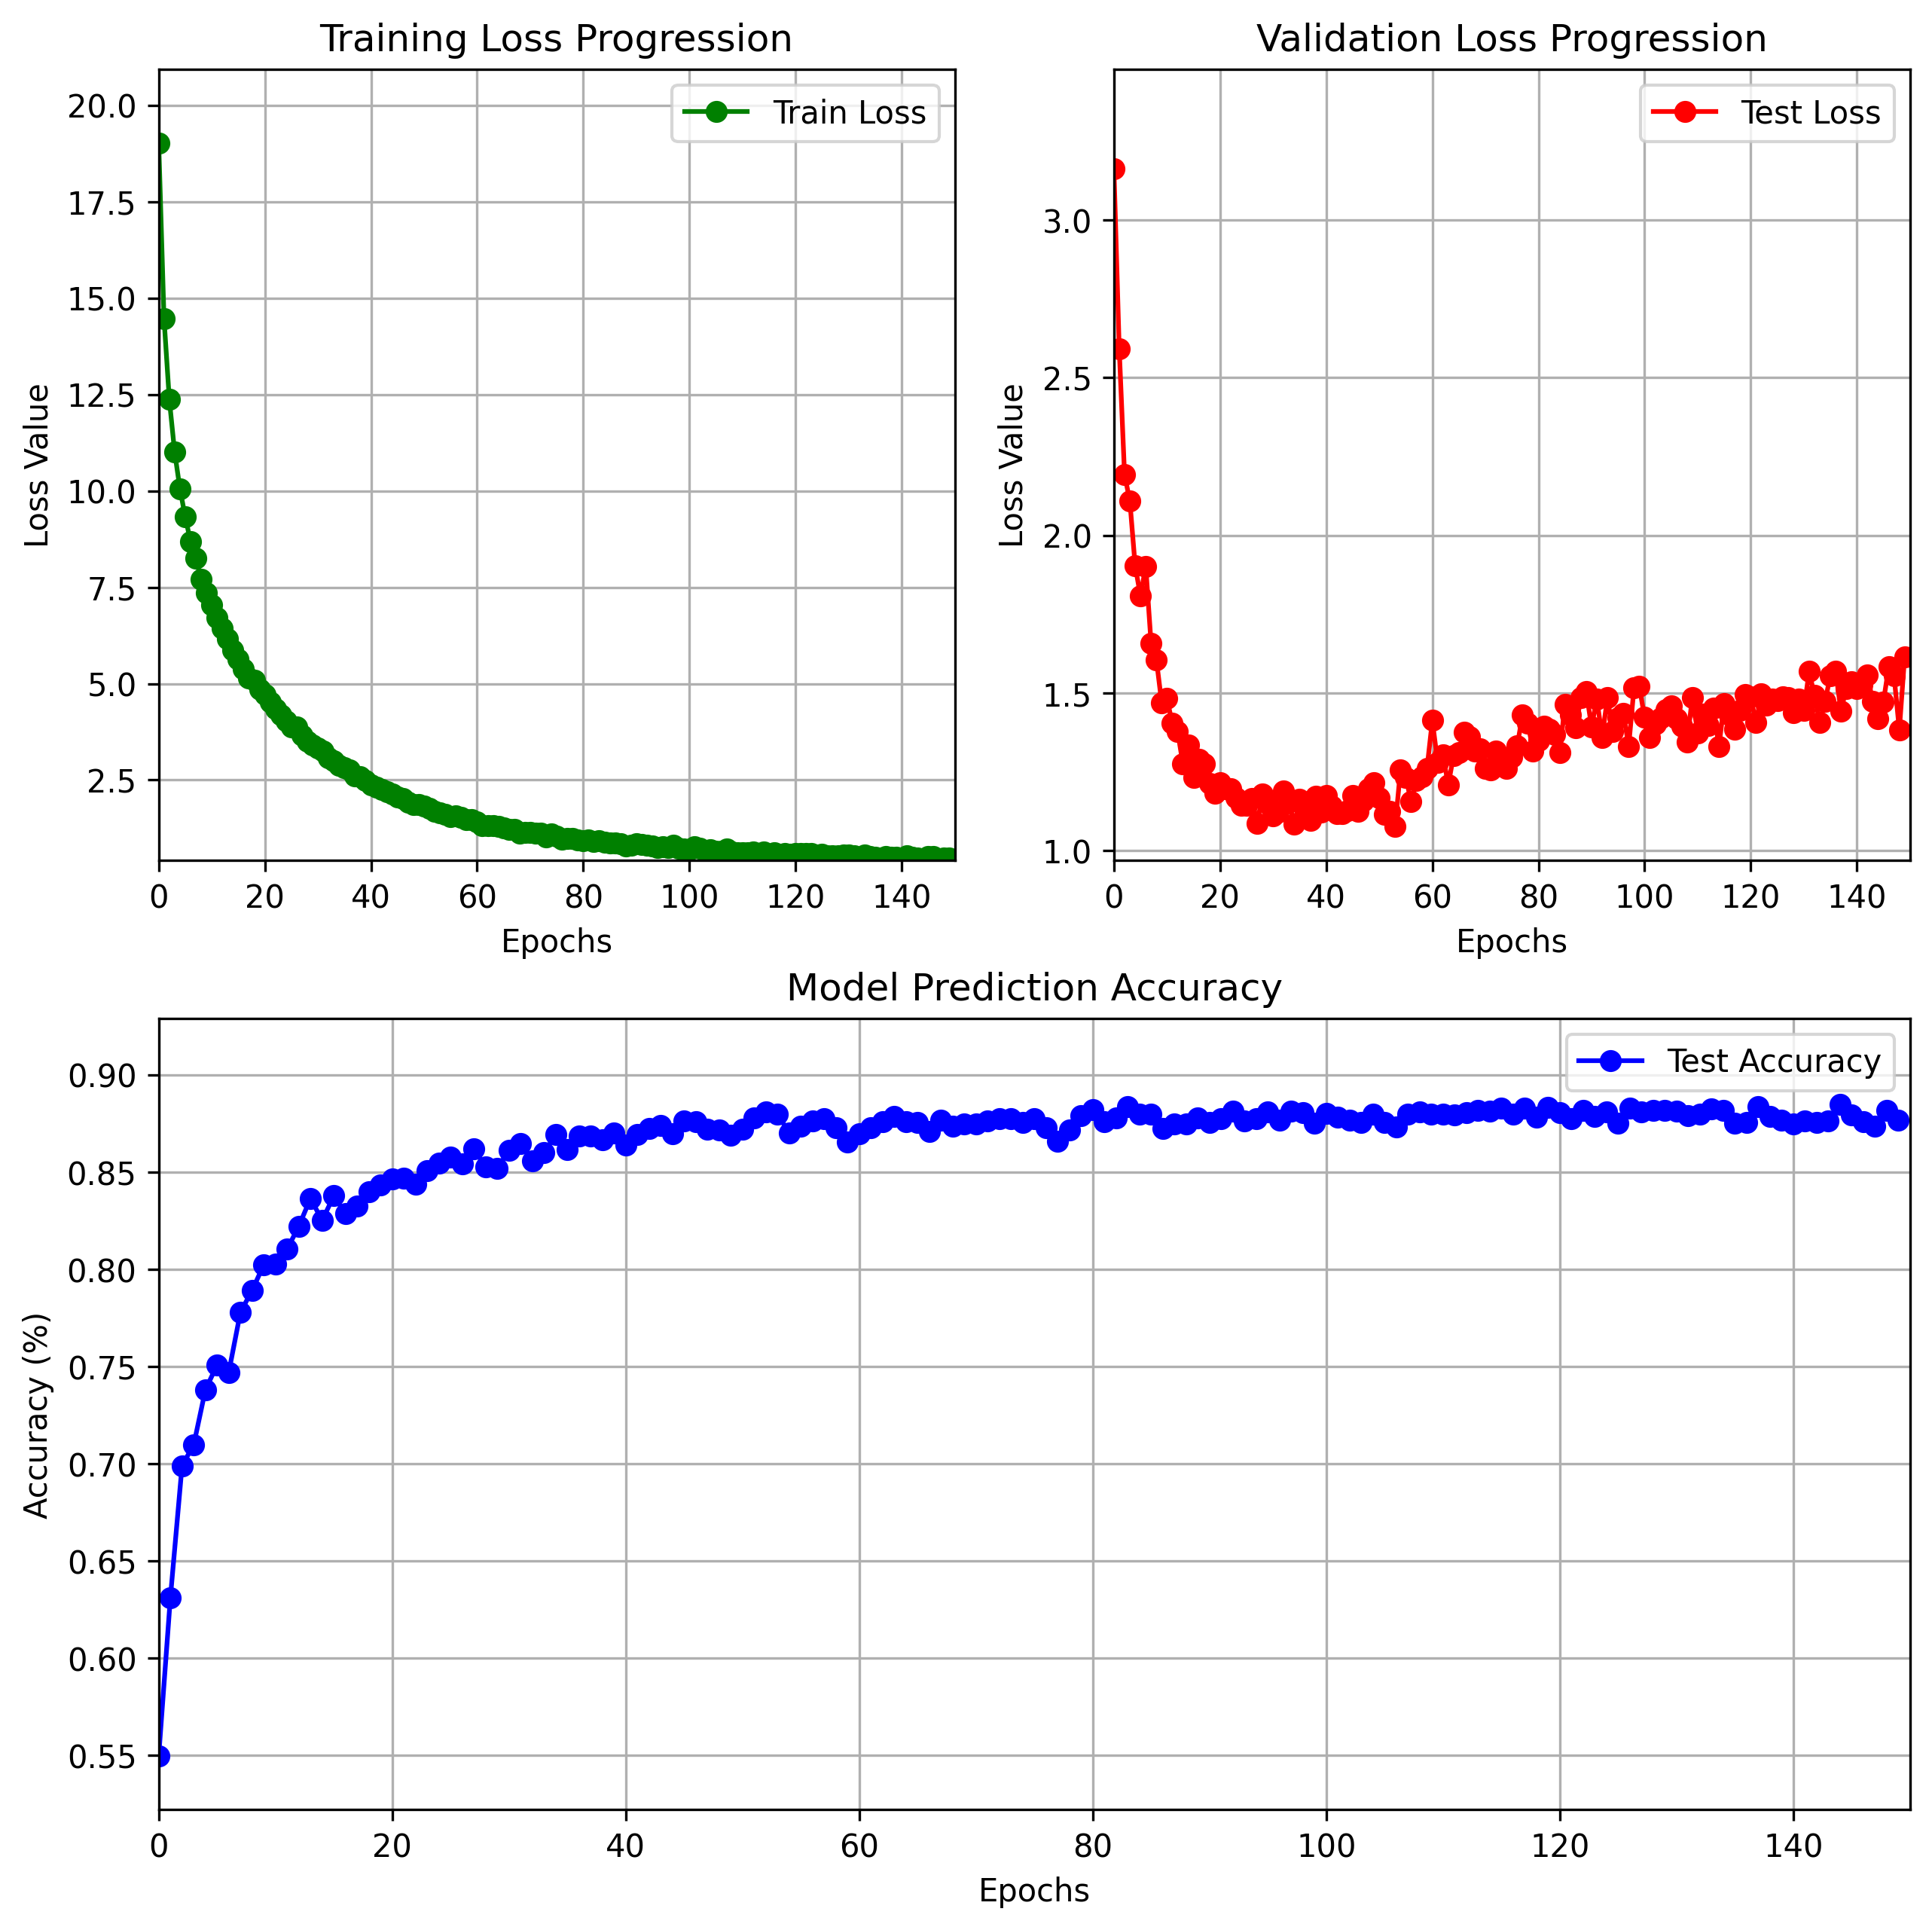
\includegraphics[width=0.45\textwidth]{fig/train_result_5.png} % 设定图片宽度
  \caption{model settings 3(left): extra data aug 5(right): no extra data aug} % 图片标题
  \label{fig:curve} % 图片标签,方便引用
\end{figure}

\noindent 3) Figure 4 shows setting 3 and 4: same in model structure and other, only differ in whether to use dropout after linear layer. It is surprising that the one without dropout has higher testing accuracy, because in common sense dropout layer will decrease overfitting. And there is no significant difference in loss curves eigther. Hence we can conclude that \textbf{dropout layer has no significant improve in our baseline model}\\

\begin{figure}[hbtp]
  \centering
  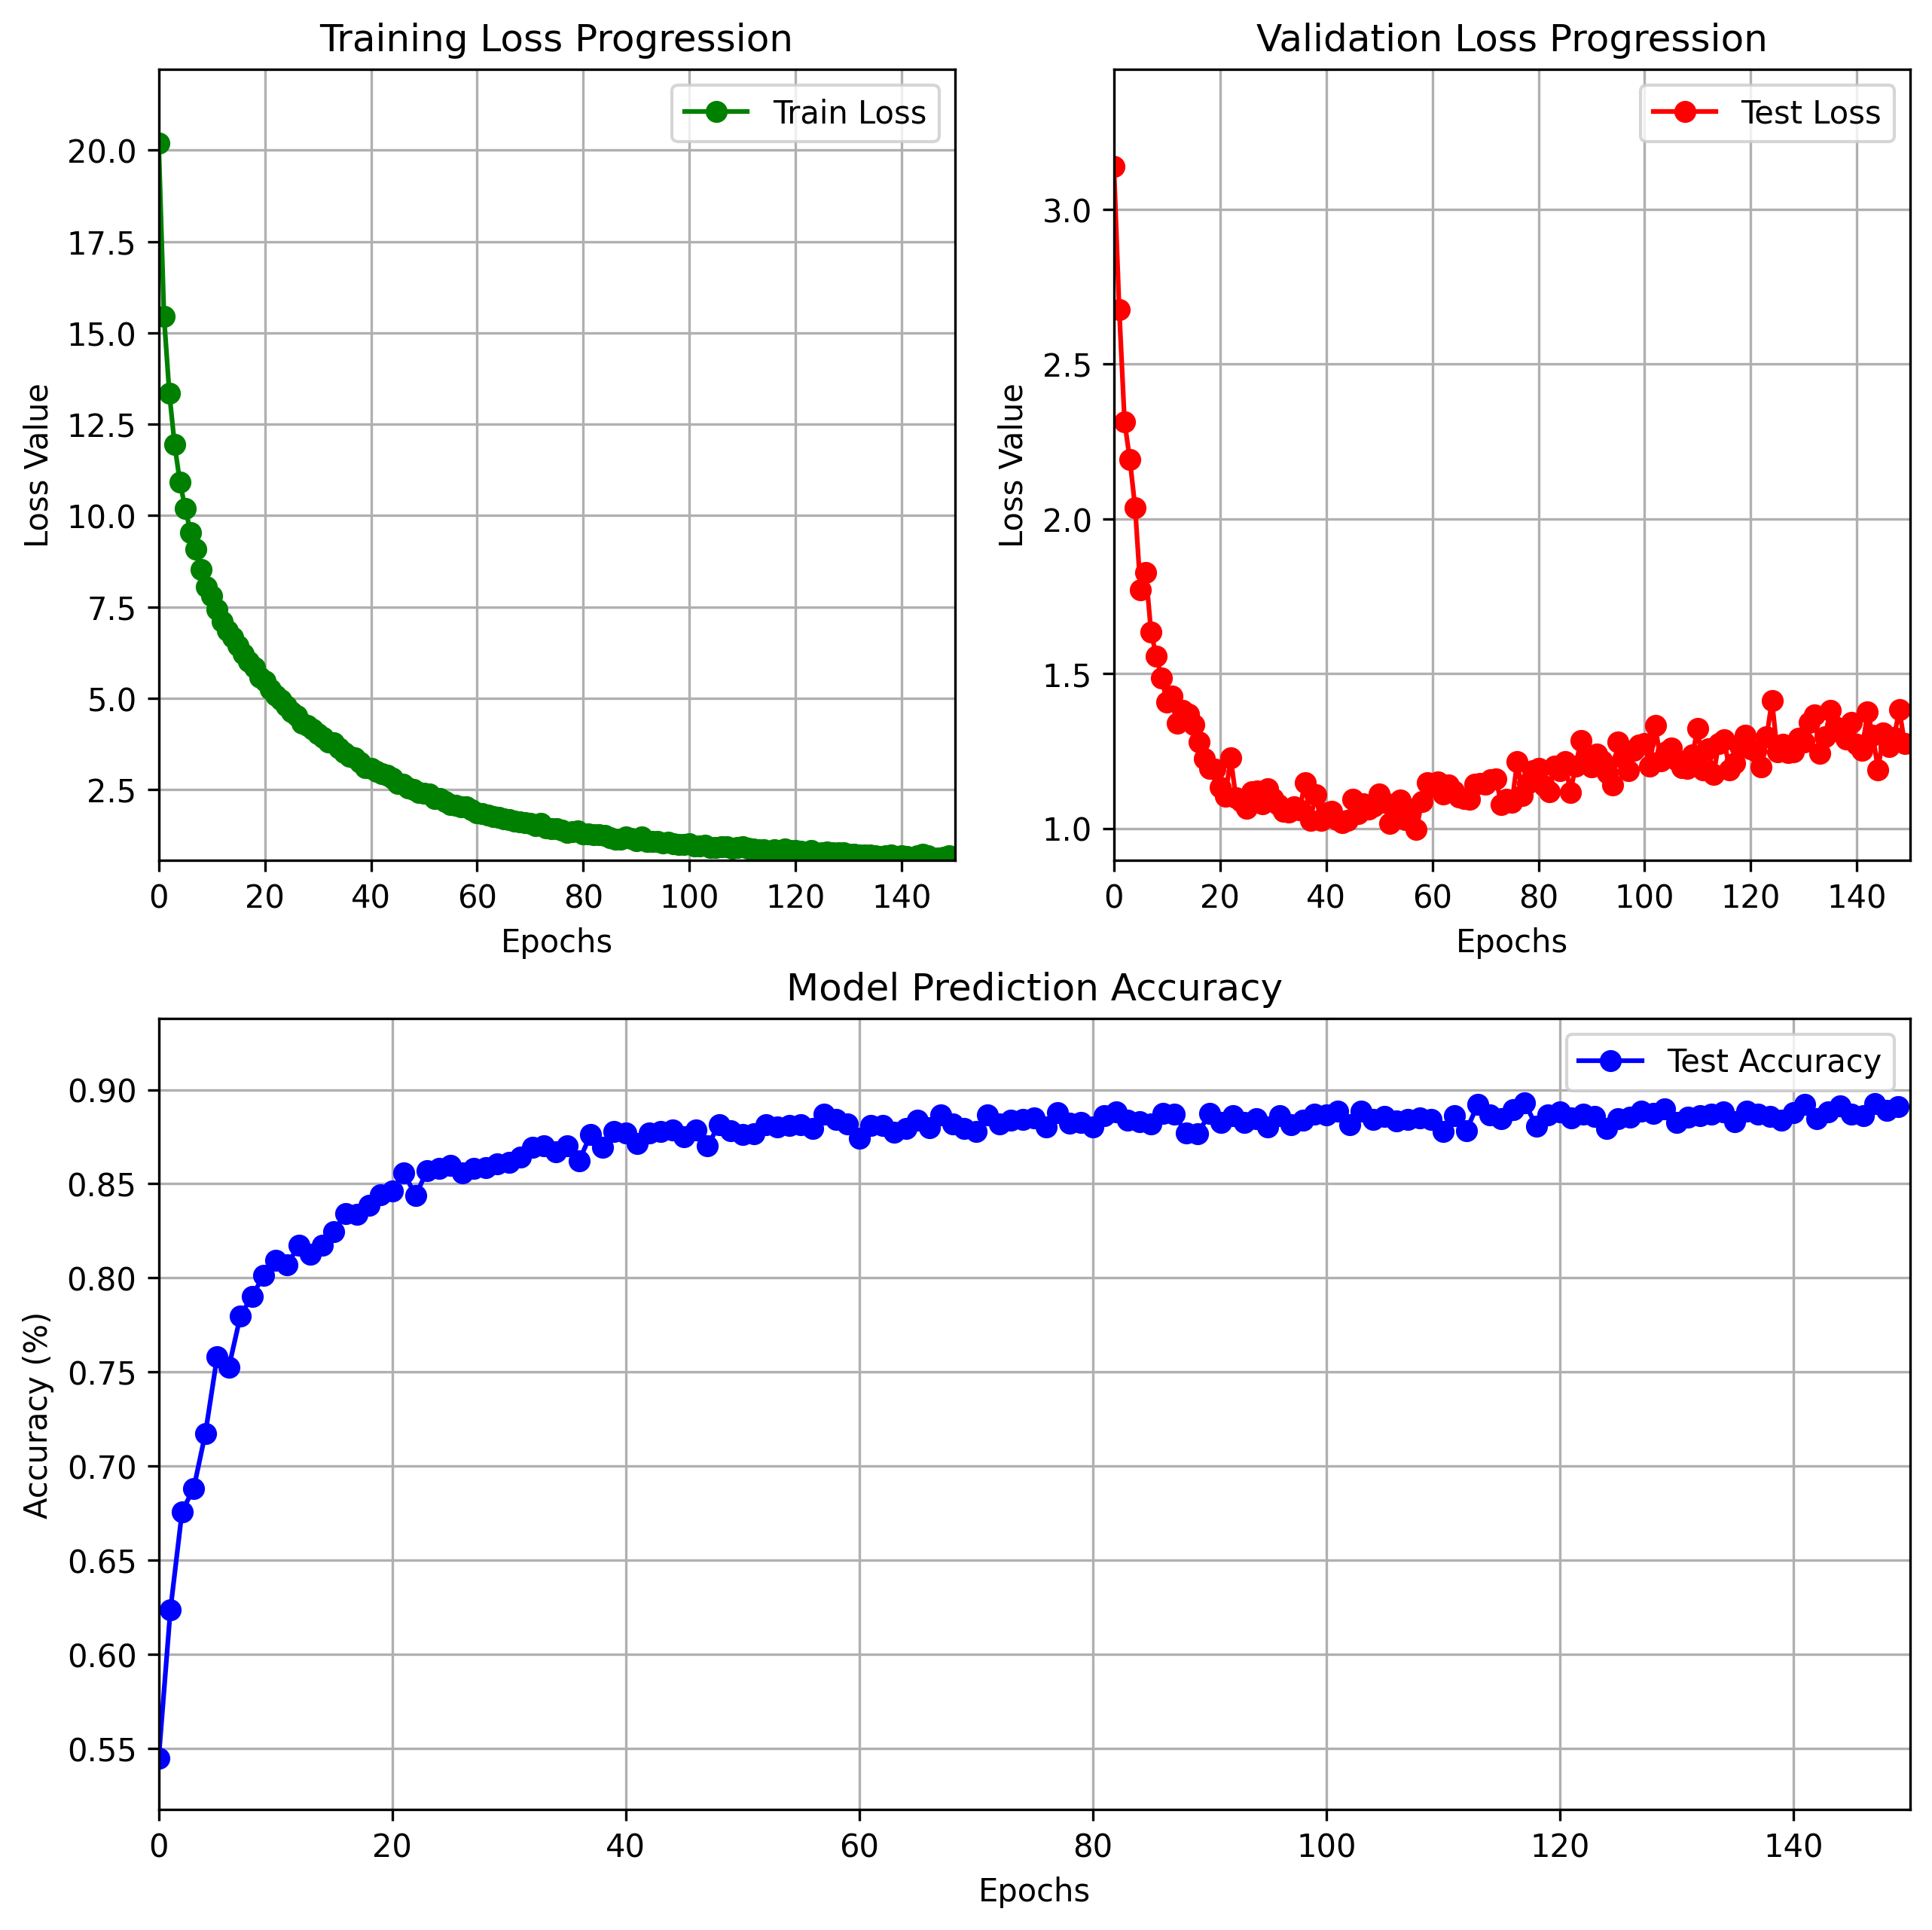
\includegraphics[width=0.45\textwidth]{fig/train_result_3.png} % 设定图片宽度
  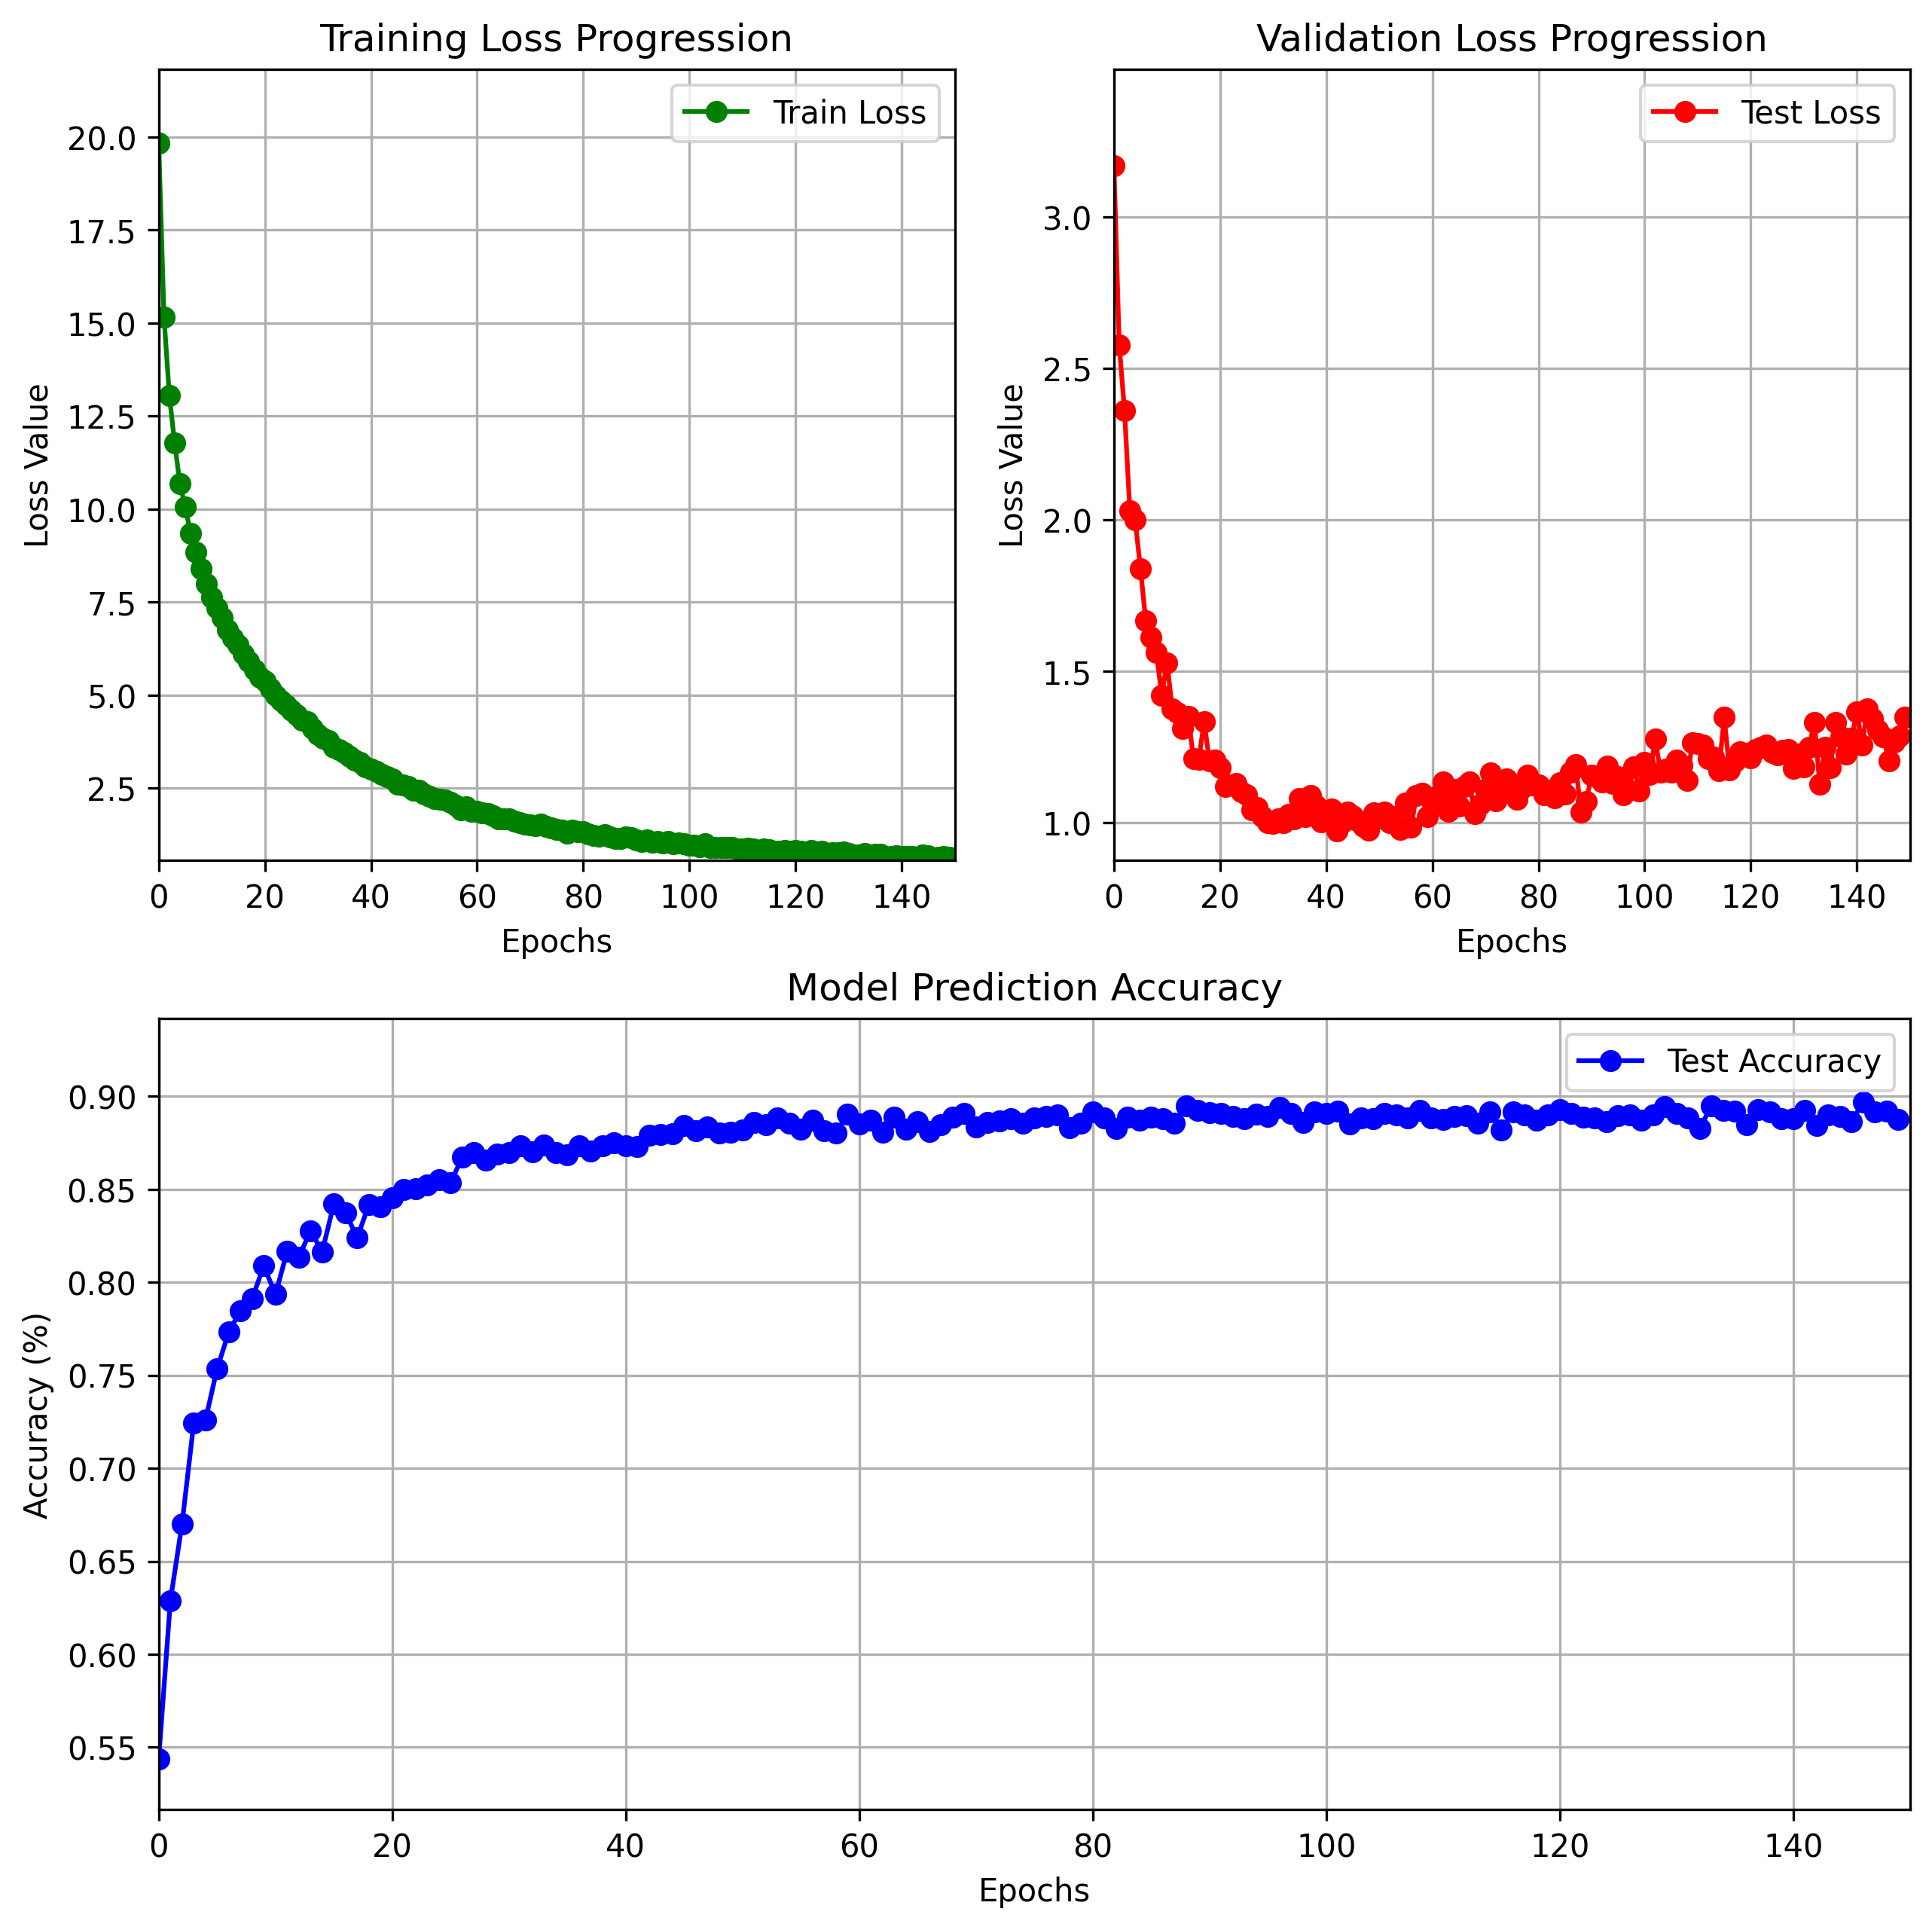
\includegraphics[width=0.45\textwidth]{fig/train_result_4.png} % 设定图片宽度
  \caption{model settings 3(left): keep only dropout after linear layer, (right): no dropout} % 图片标题
  \label{fig:curve} % 图片标签,方便引用
\end{figure}

\noindent 4) At Figure 5, we also add more training epochs to our \textcolor{blue}{BEST} model: \textbf{Why we choose setting 3 to be the BEST? Although setting 3 has better accuracy, but only better in a margin, but dropoutput can accelerate training, because it "dropout" 50\% params in linear layer.} the BEST model is the same with setting 3, only differ in number of training epoch, we add 100 more epoch to see if the testing accuracy can go higher. But find out the best testing accuracy didn't improve, and never go beyond 90\%, it converges to 89.5\%.\\


\begin{figure}[hbtp]
  \centering
  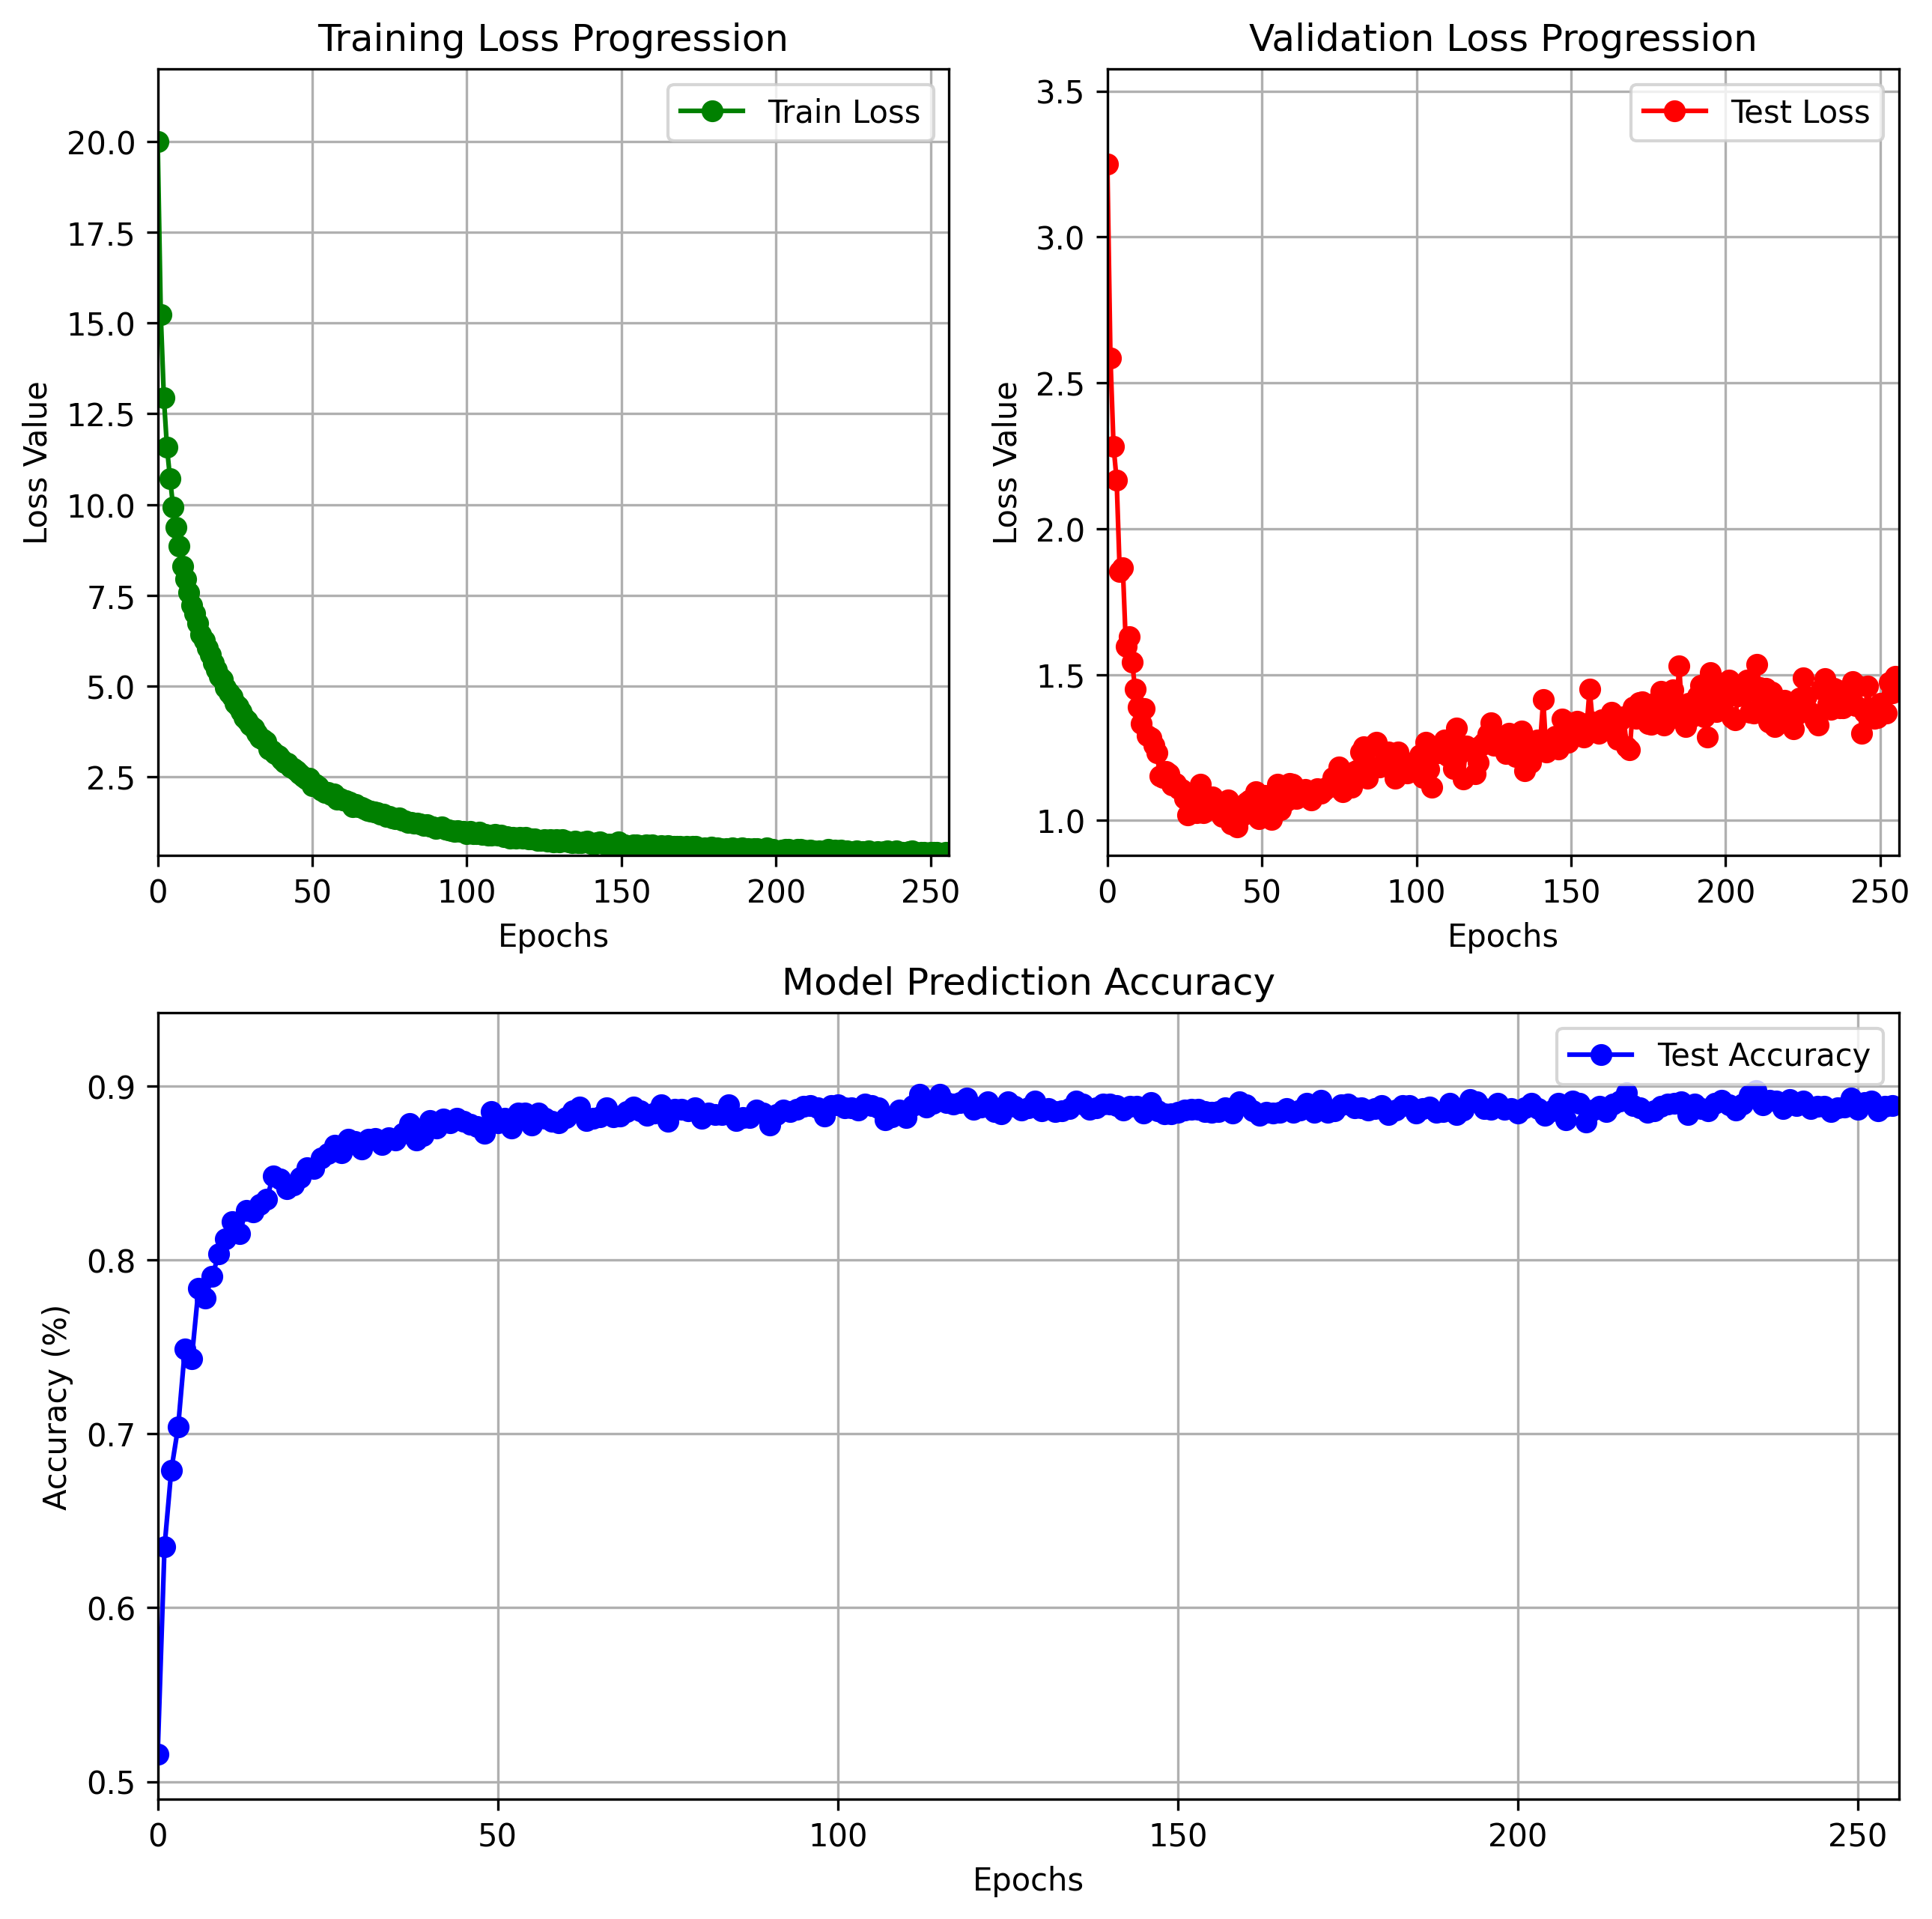
\includegraphics[width=0.45\textwidth]{fig/train_result_6.png} % 设定图片宽度

  \caption{model settings 6: BEST model (same with setting 3) with more training epochs} % 图片标题
  \label{fig:curve} % 图片标签,方便引用
\end{figure}

\noindent 5) At Figure 6: since dropout layer has no much difference to model performance, by comparing setting 1 and setting 3, we can conclude that \textcolor{blue}{BatchNorm has significant improvement to testing accuracy.} \\

\begin{figure}[hbtp]
  \centering
  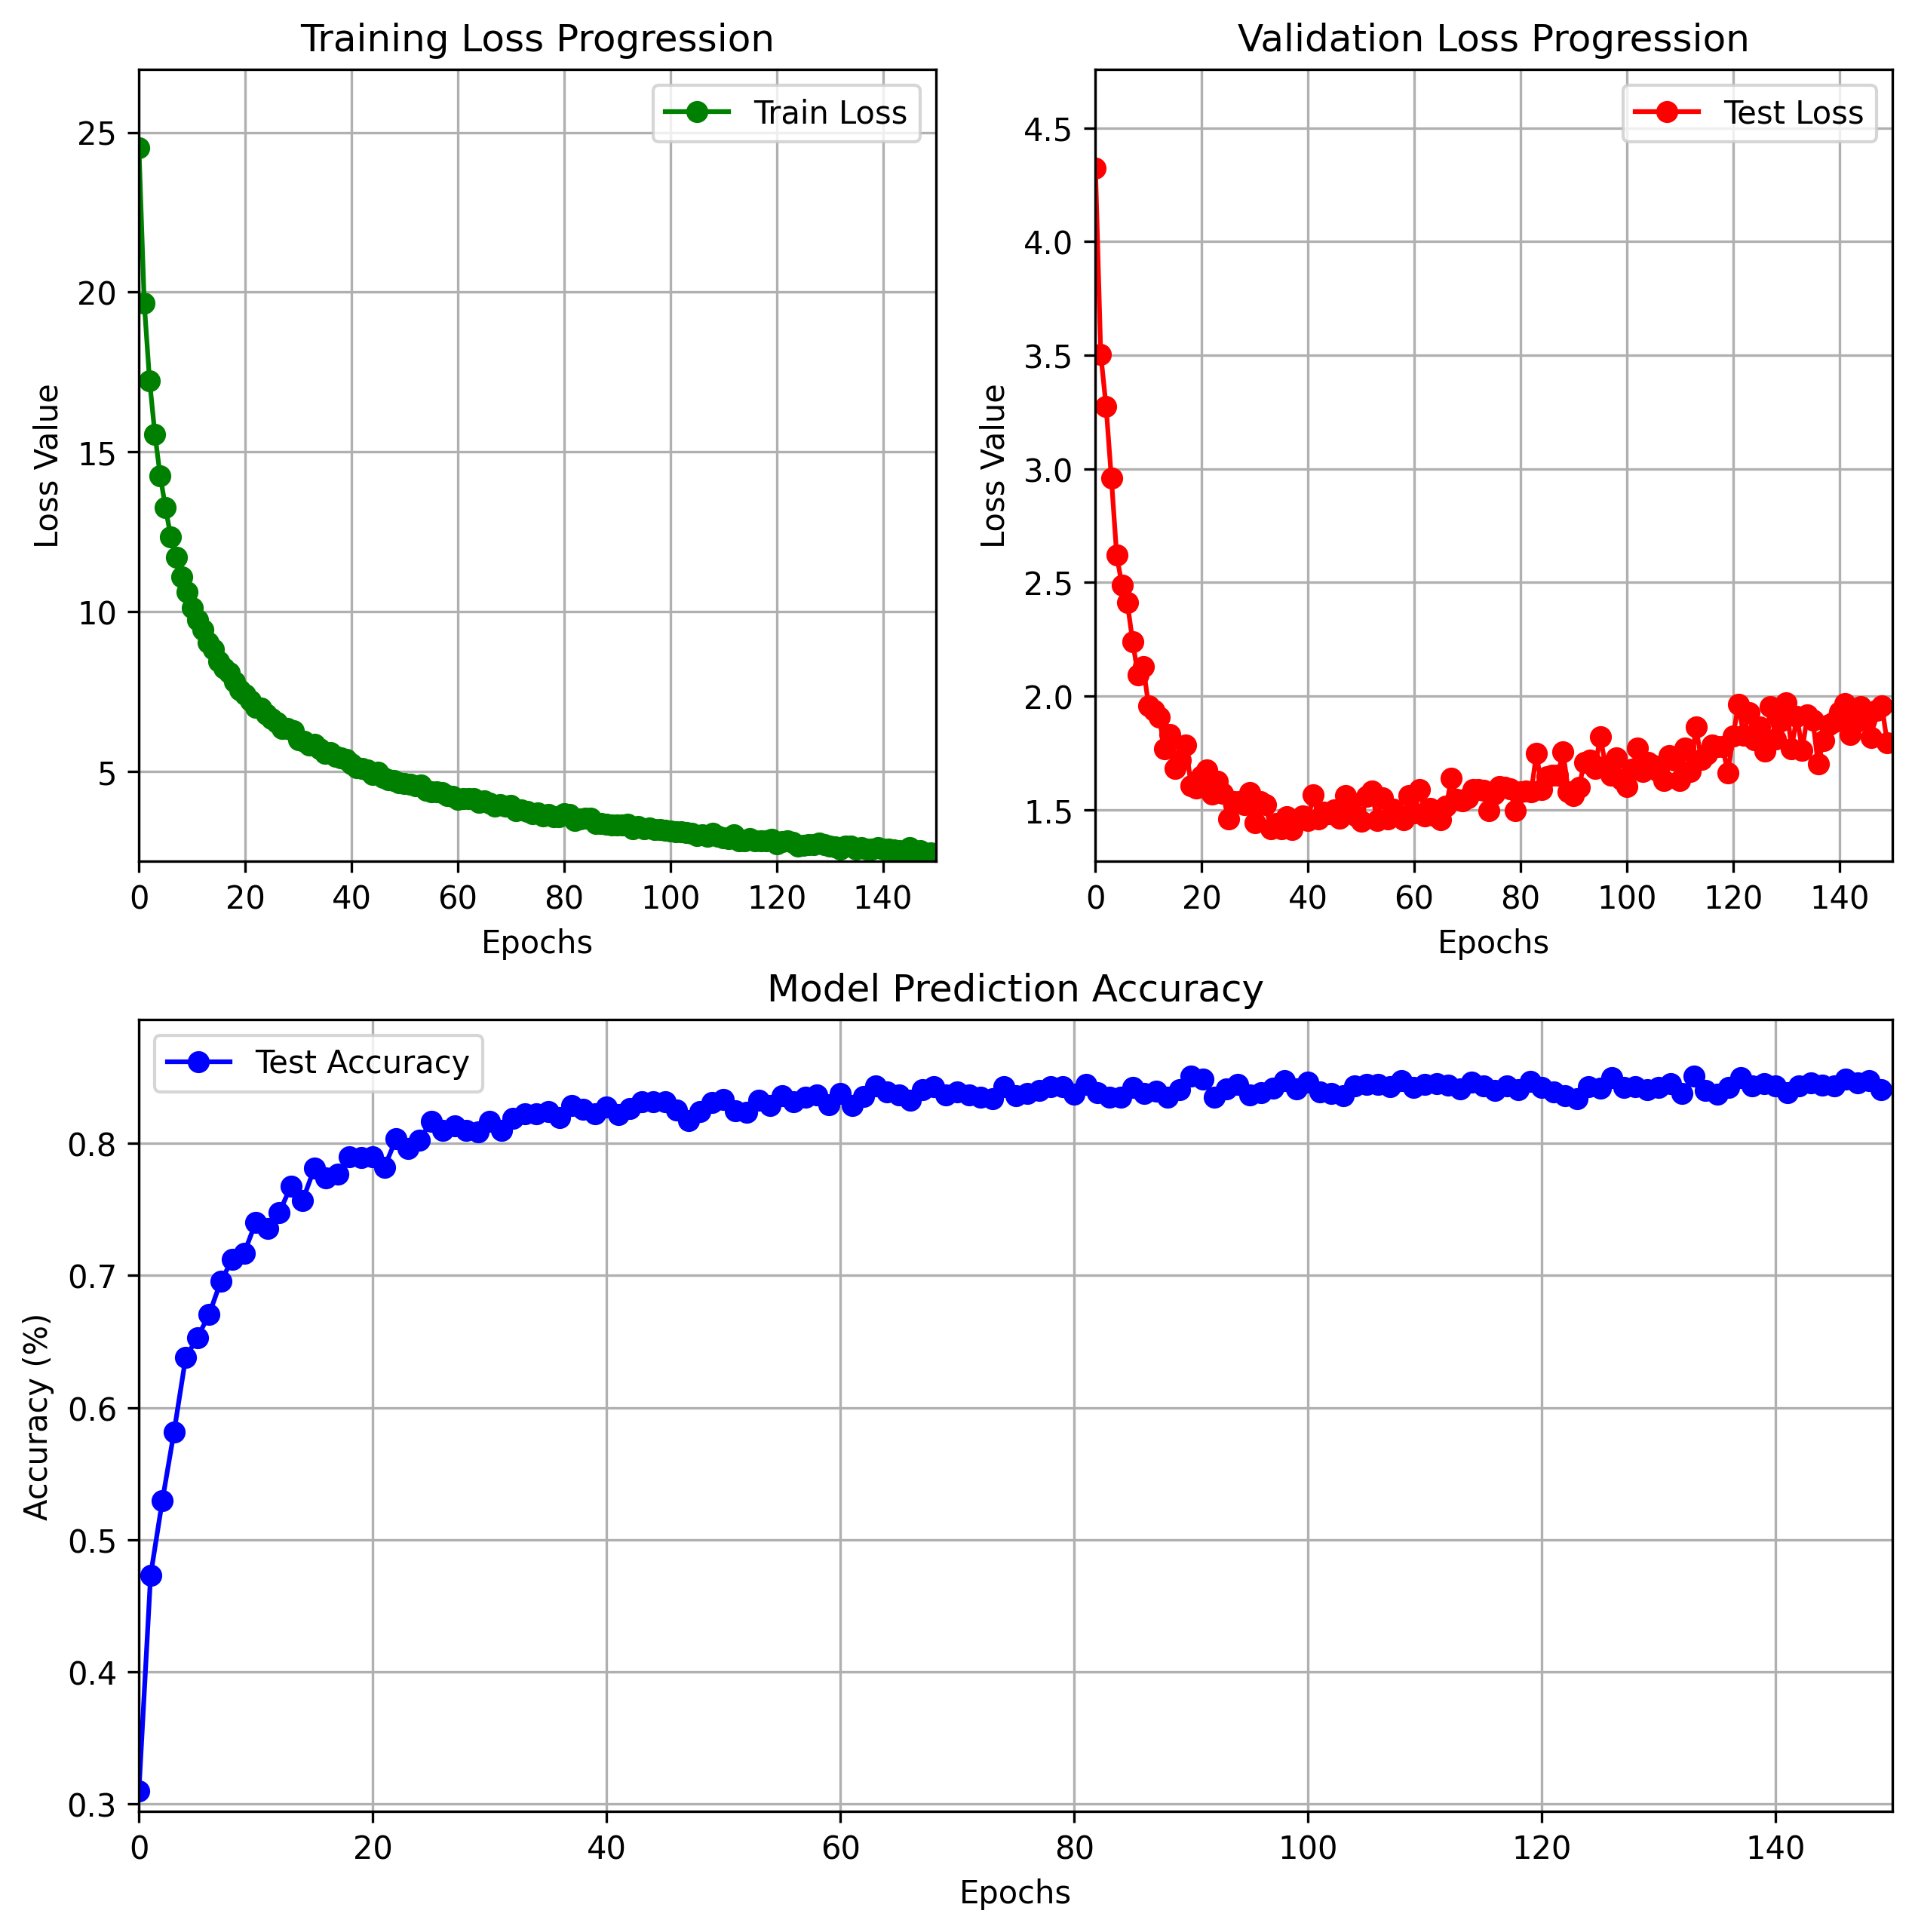
\includegraphics[width=0.45\textwidth]{fig/train_result_1.png} % 设定图片宽度
  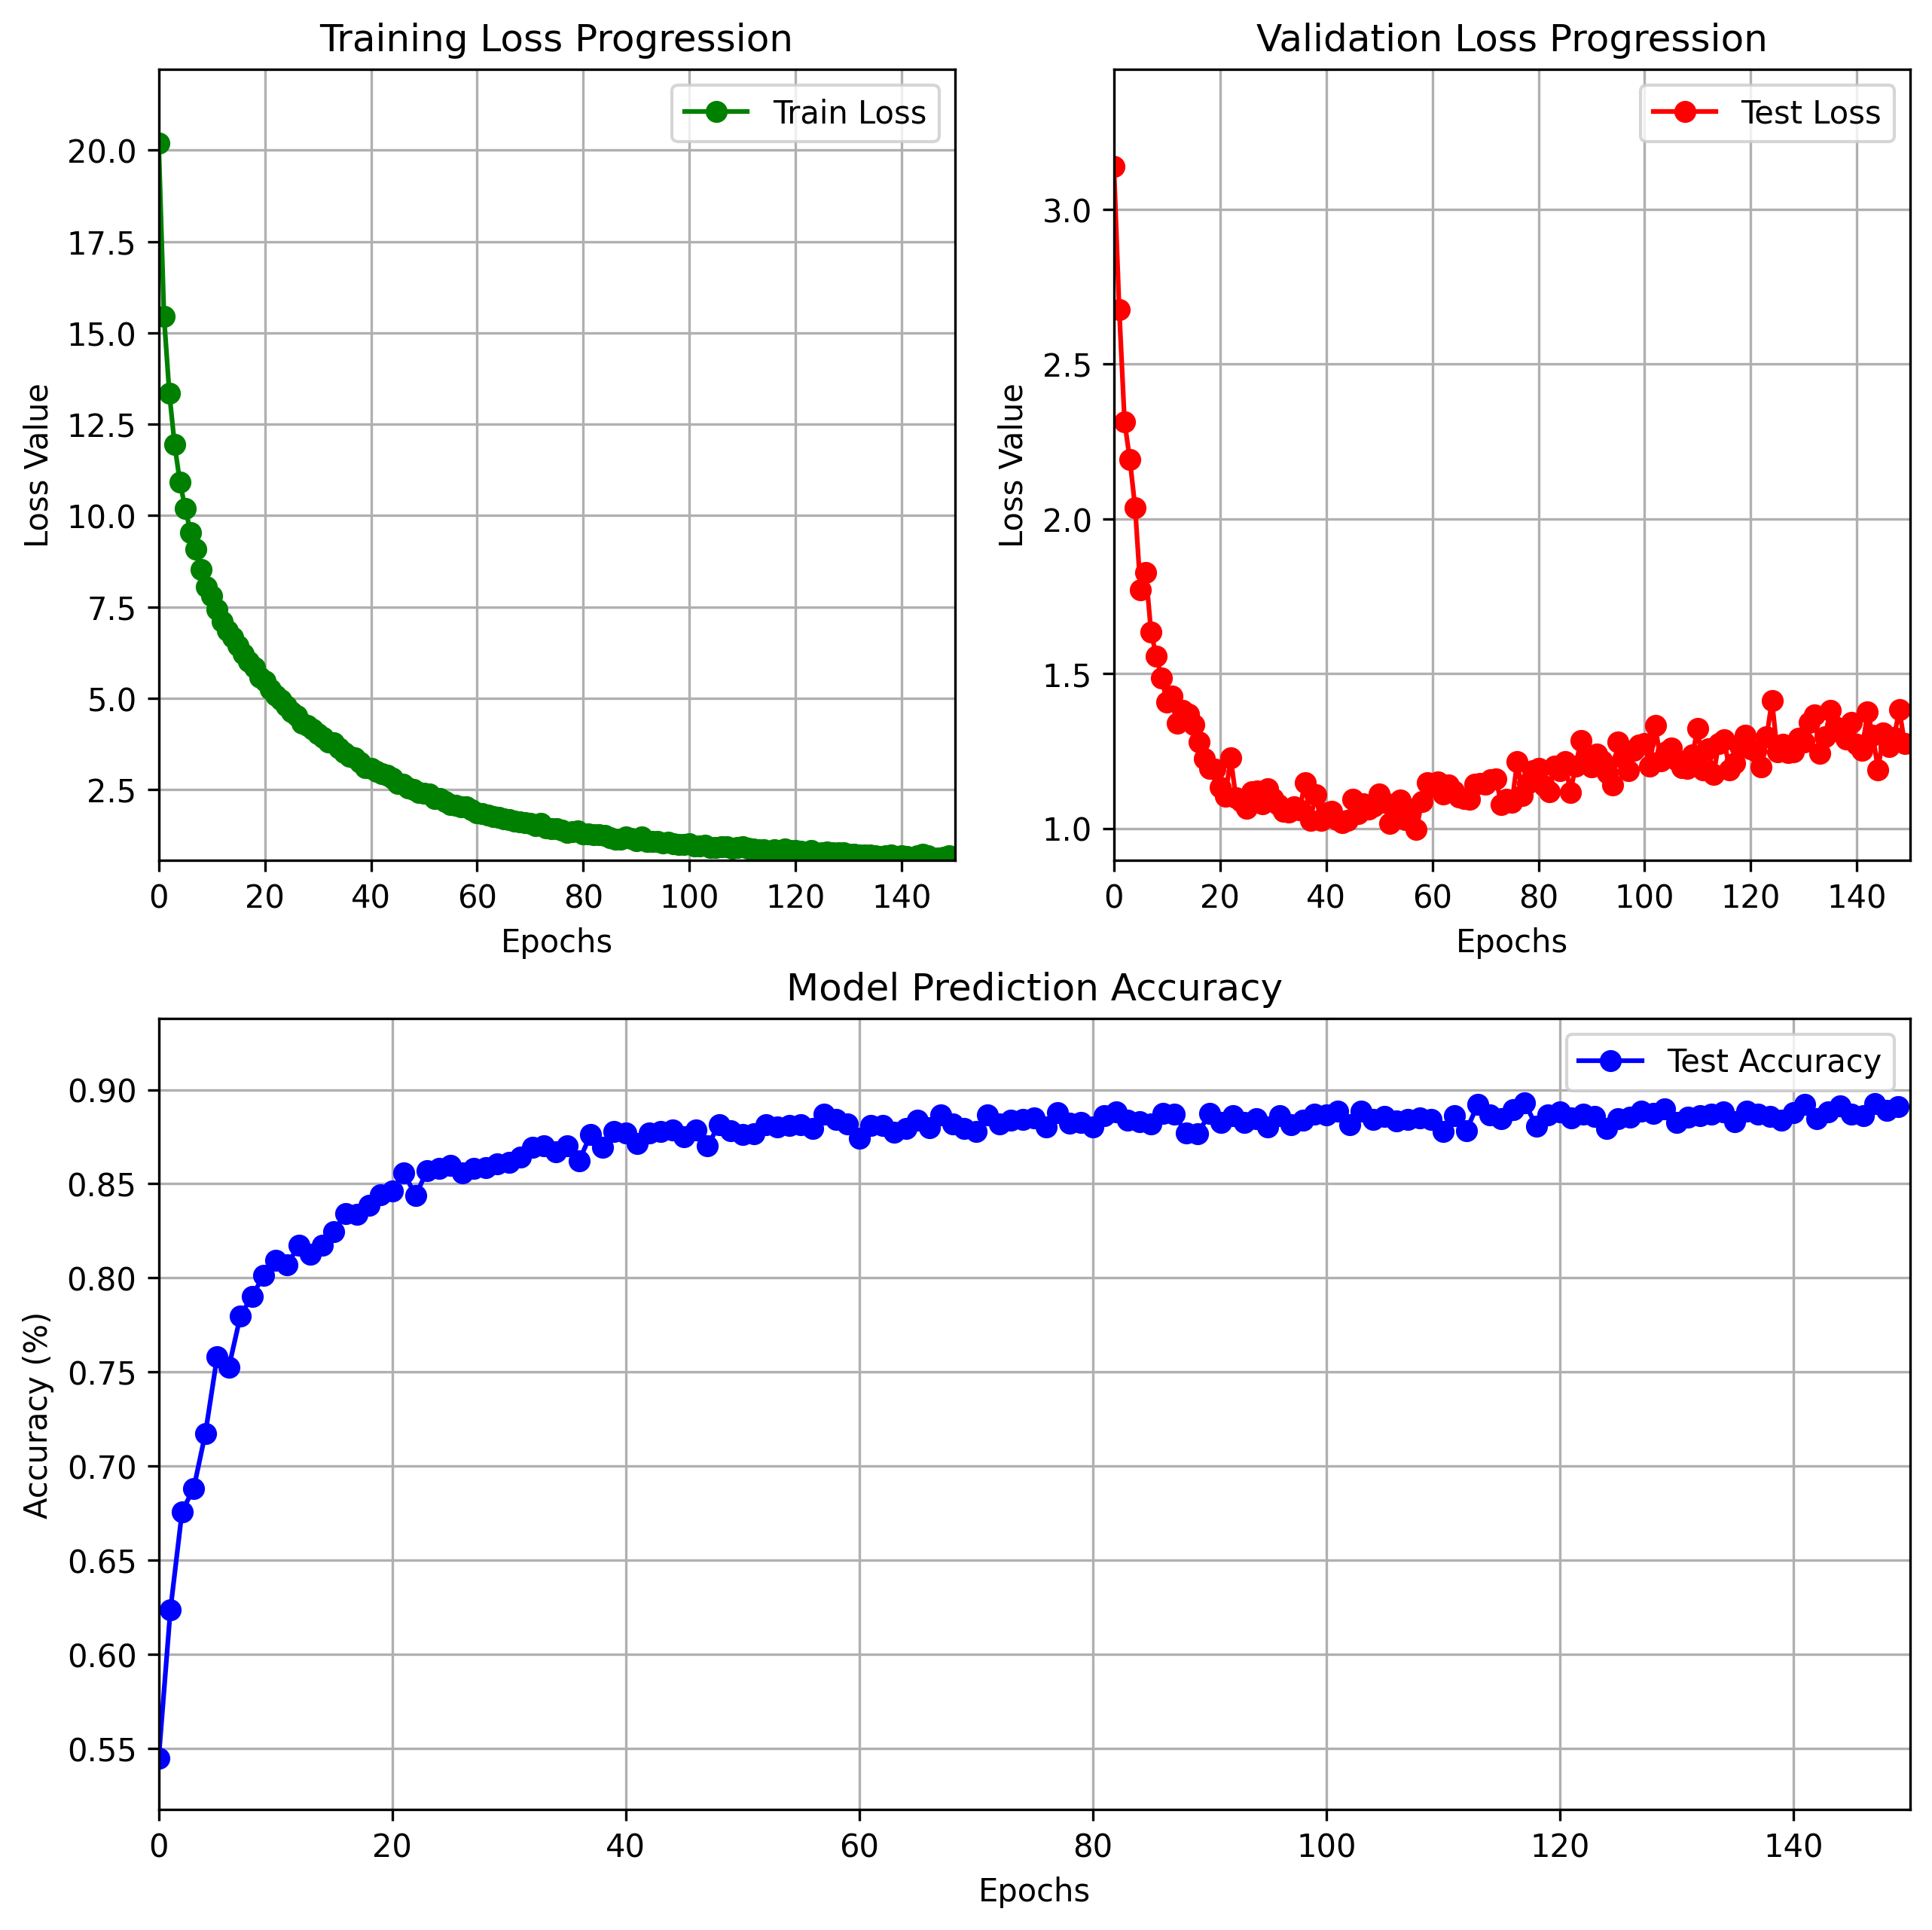
\includegraphics[width=0.45\textwidth]{fig/train_result_3.png} % 设定图片宽度
  \caption{model settings 1(left): no Batchnorm, setting 3(right): with Batchnorm} % 图片标题
  \label{fig:curve} % 图片标签,方便引用
\end{figure}




\textcolor{red}{\# Note:} bacthsize = 64, Epoch num = 150, dropout(conv) indicate whether we use dropout layer in convlution layer.

\noindent - Baseline Model Results Interpretation: 
\begin{itemize}
  \item BatchNorm considerably improve accuracy (+4.5\%), compared with other techniques.
  \item choosing SGD or Adam will not significantly affect accuracy, they just converge to almost the same accuracy at different speeds (in terms of epochs). \textcolor{blue}{attach figure of loss curve}
  \item dropout layers have almost no effect to the performance of model, since we have tested 2 scenarios: 1) keep dropout layers only in Linear layer (popular method) 2) removing all dropout layers; and they do not differ much in terms of test accu.
  \item Notice that the last column of the table, we re-do the 3rd settings for 256 epochs, and the test accuracy only improve for a margin. (almost no improvement)
\end{itemize}

% ============== use advanced model structure: vgg16/resnet18/resnet50 ================
\subs{2.3 Deeper Neural Network}
Although our basline model can achieve around 90\% accuracy on test set, deeper neural network can always (at a high prob) handle complicated features better, here, cifar-10 images have complex features. So we decided to try deeper networks \texttt{vgg16, ResNet18, ResNet50}.

\texttt{vgg16} stacking 5 blocks of conv->batchnorm->relu->conv->batchnorm->relu->maxpool, hoping to extract more abstract representation of features.

\texttt{ResNet18} stacking 4 basic ResidualBlocks, by doing so it allows gradient to propagate without exploding or disappearing.

\texttt{ResNet50} stack 4 special ResidualBlock (named BottleNeck Block) and allows gradient to propagate in even deeper network.\\

\noindent The training and testing results are shown in below Table 2 + Figure 7.

\begin{table}[htbp]
  \centering
  \caption{ModelSettings and Performance on cifar-10}
  \label{tab:model-compare}
  \begin{tabular}{|c|ccc|} 
    \hline
    Model & vgg16 & ResNet18 & ResNet50  \\
    \hline
    TestAcc & 91.01 & 92.51 & 92.29  \\
    \hline
  \end{tabular} 
\end{table}

\begin{figure}[H]
  \centering
  
  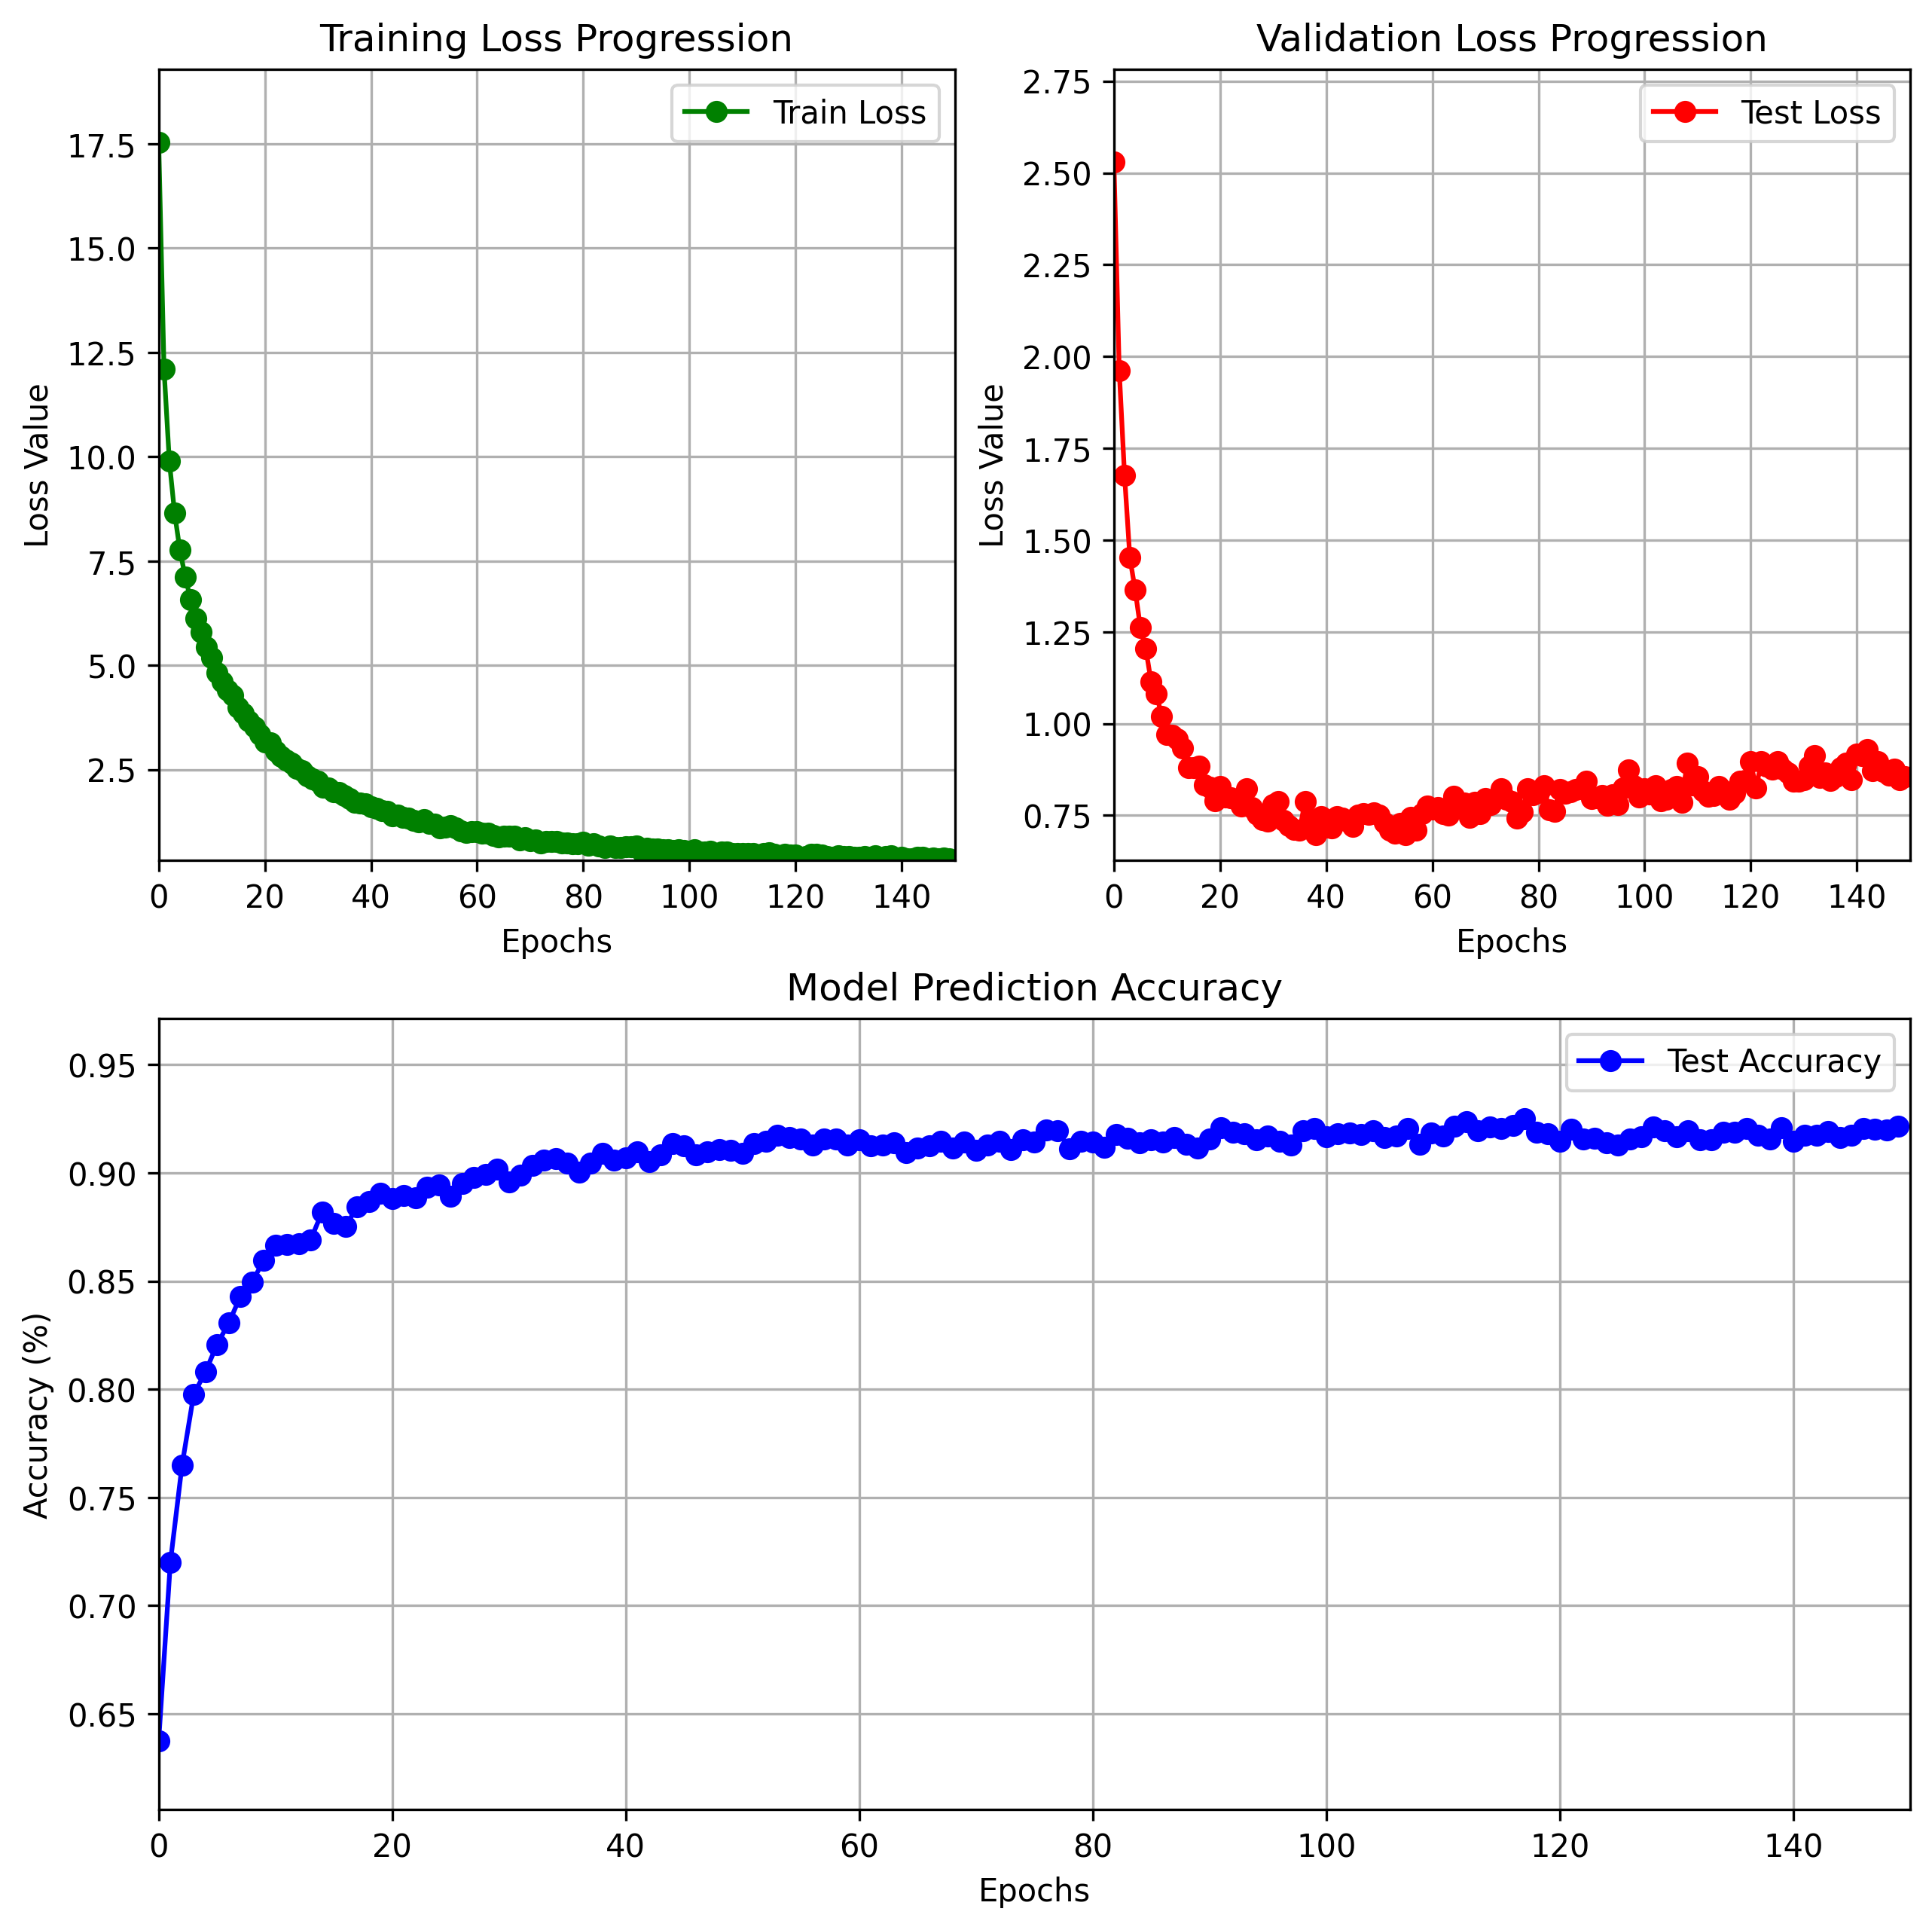
\includegraphics[width=0.3\textwidth]{fig/train_result_res18.png} % 设定图片宽度
  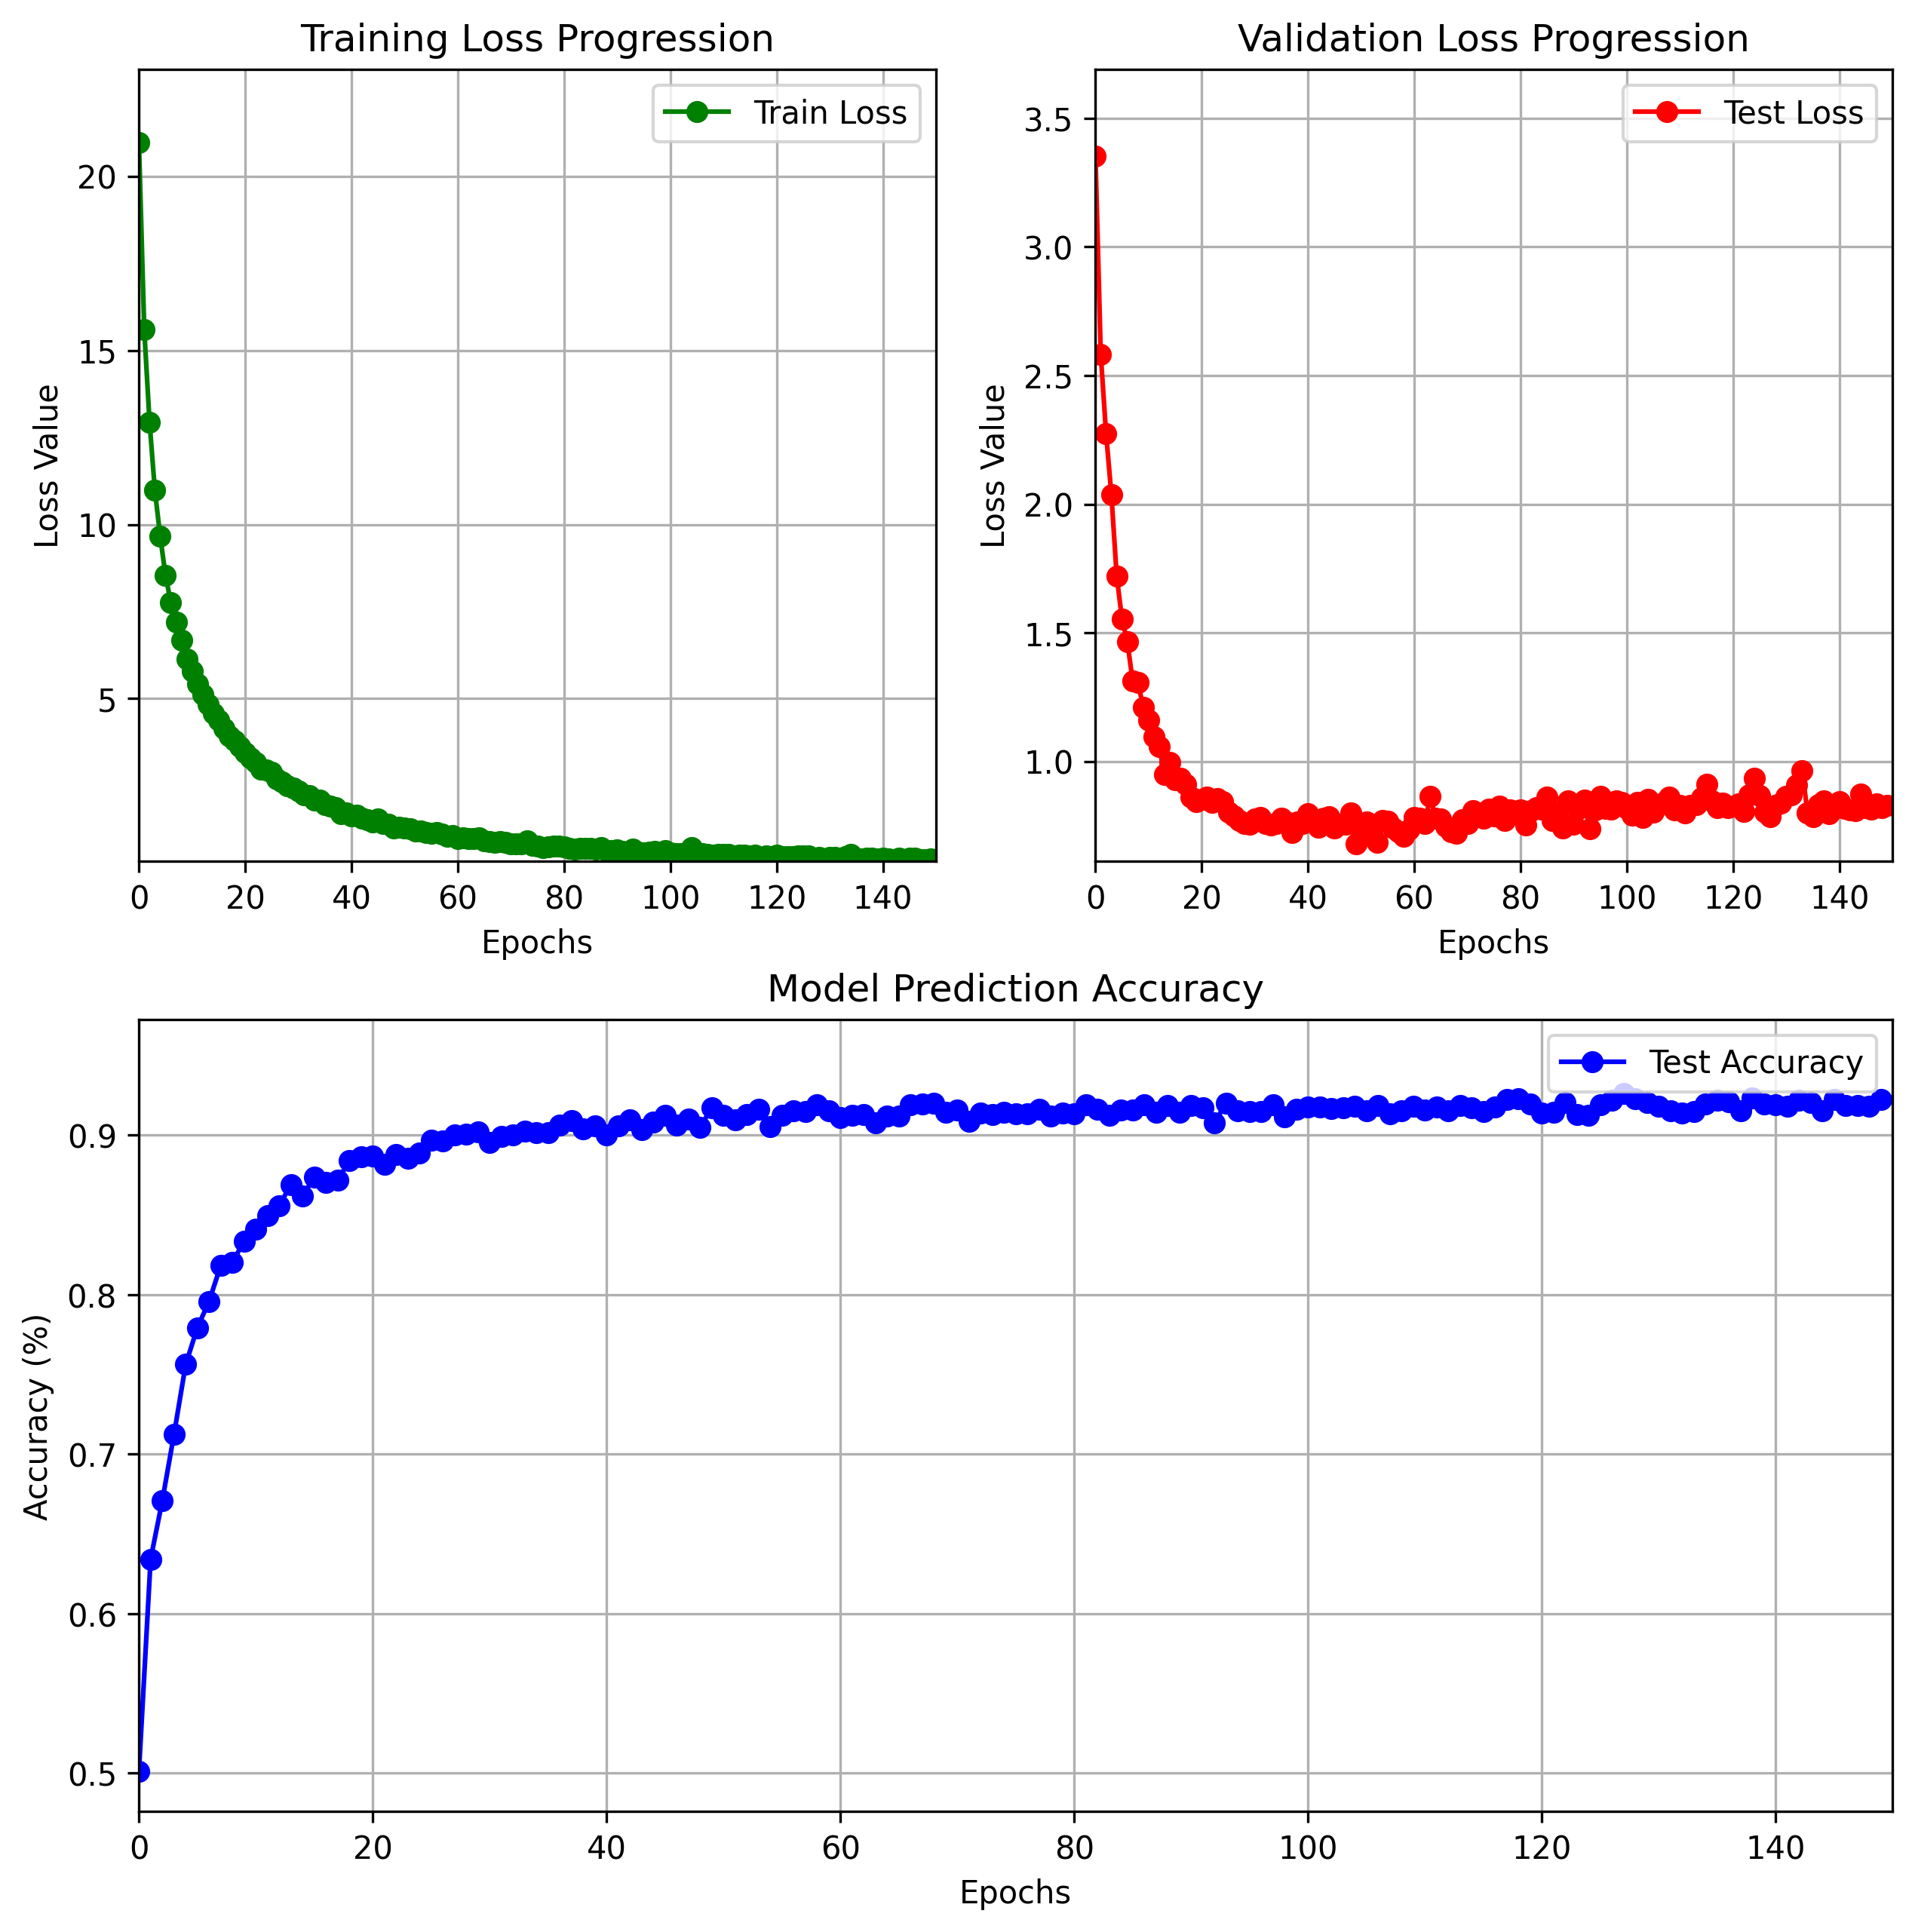
\includegraphics[width=0.3\textwidth]{fig/train_result_res50.png} % 设定图片宽度
  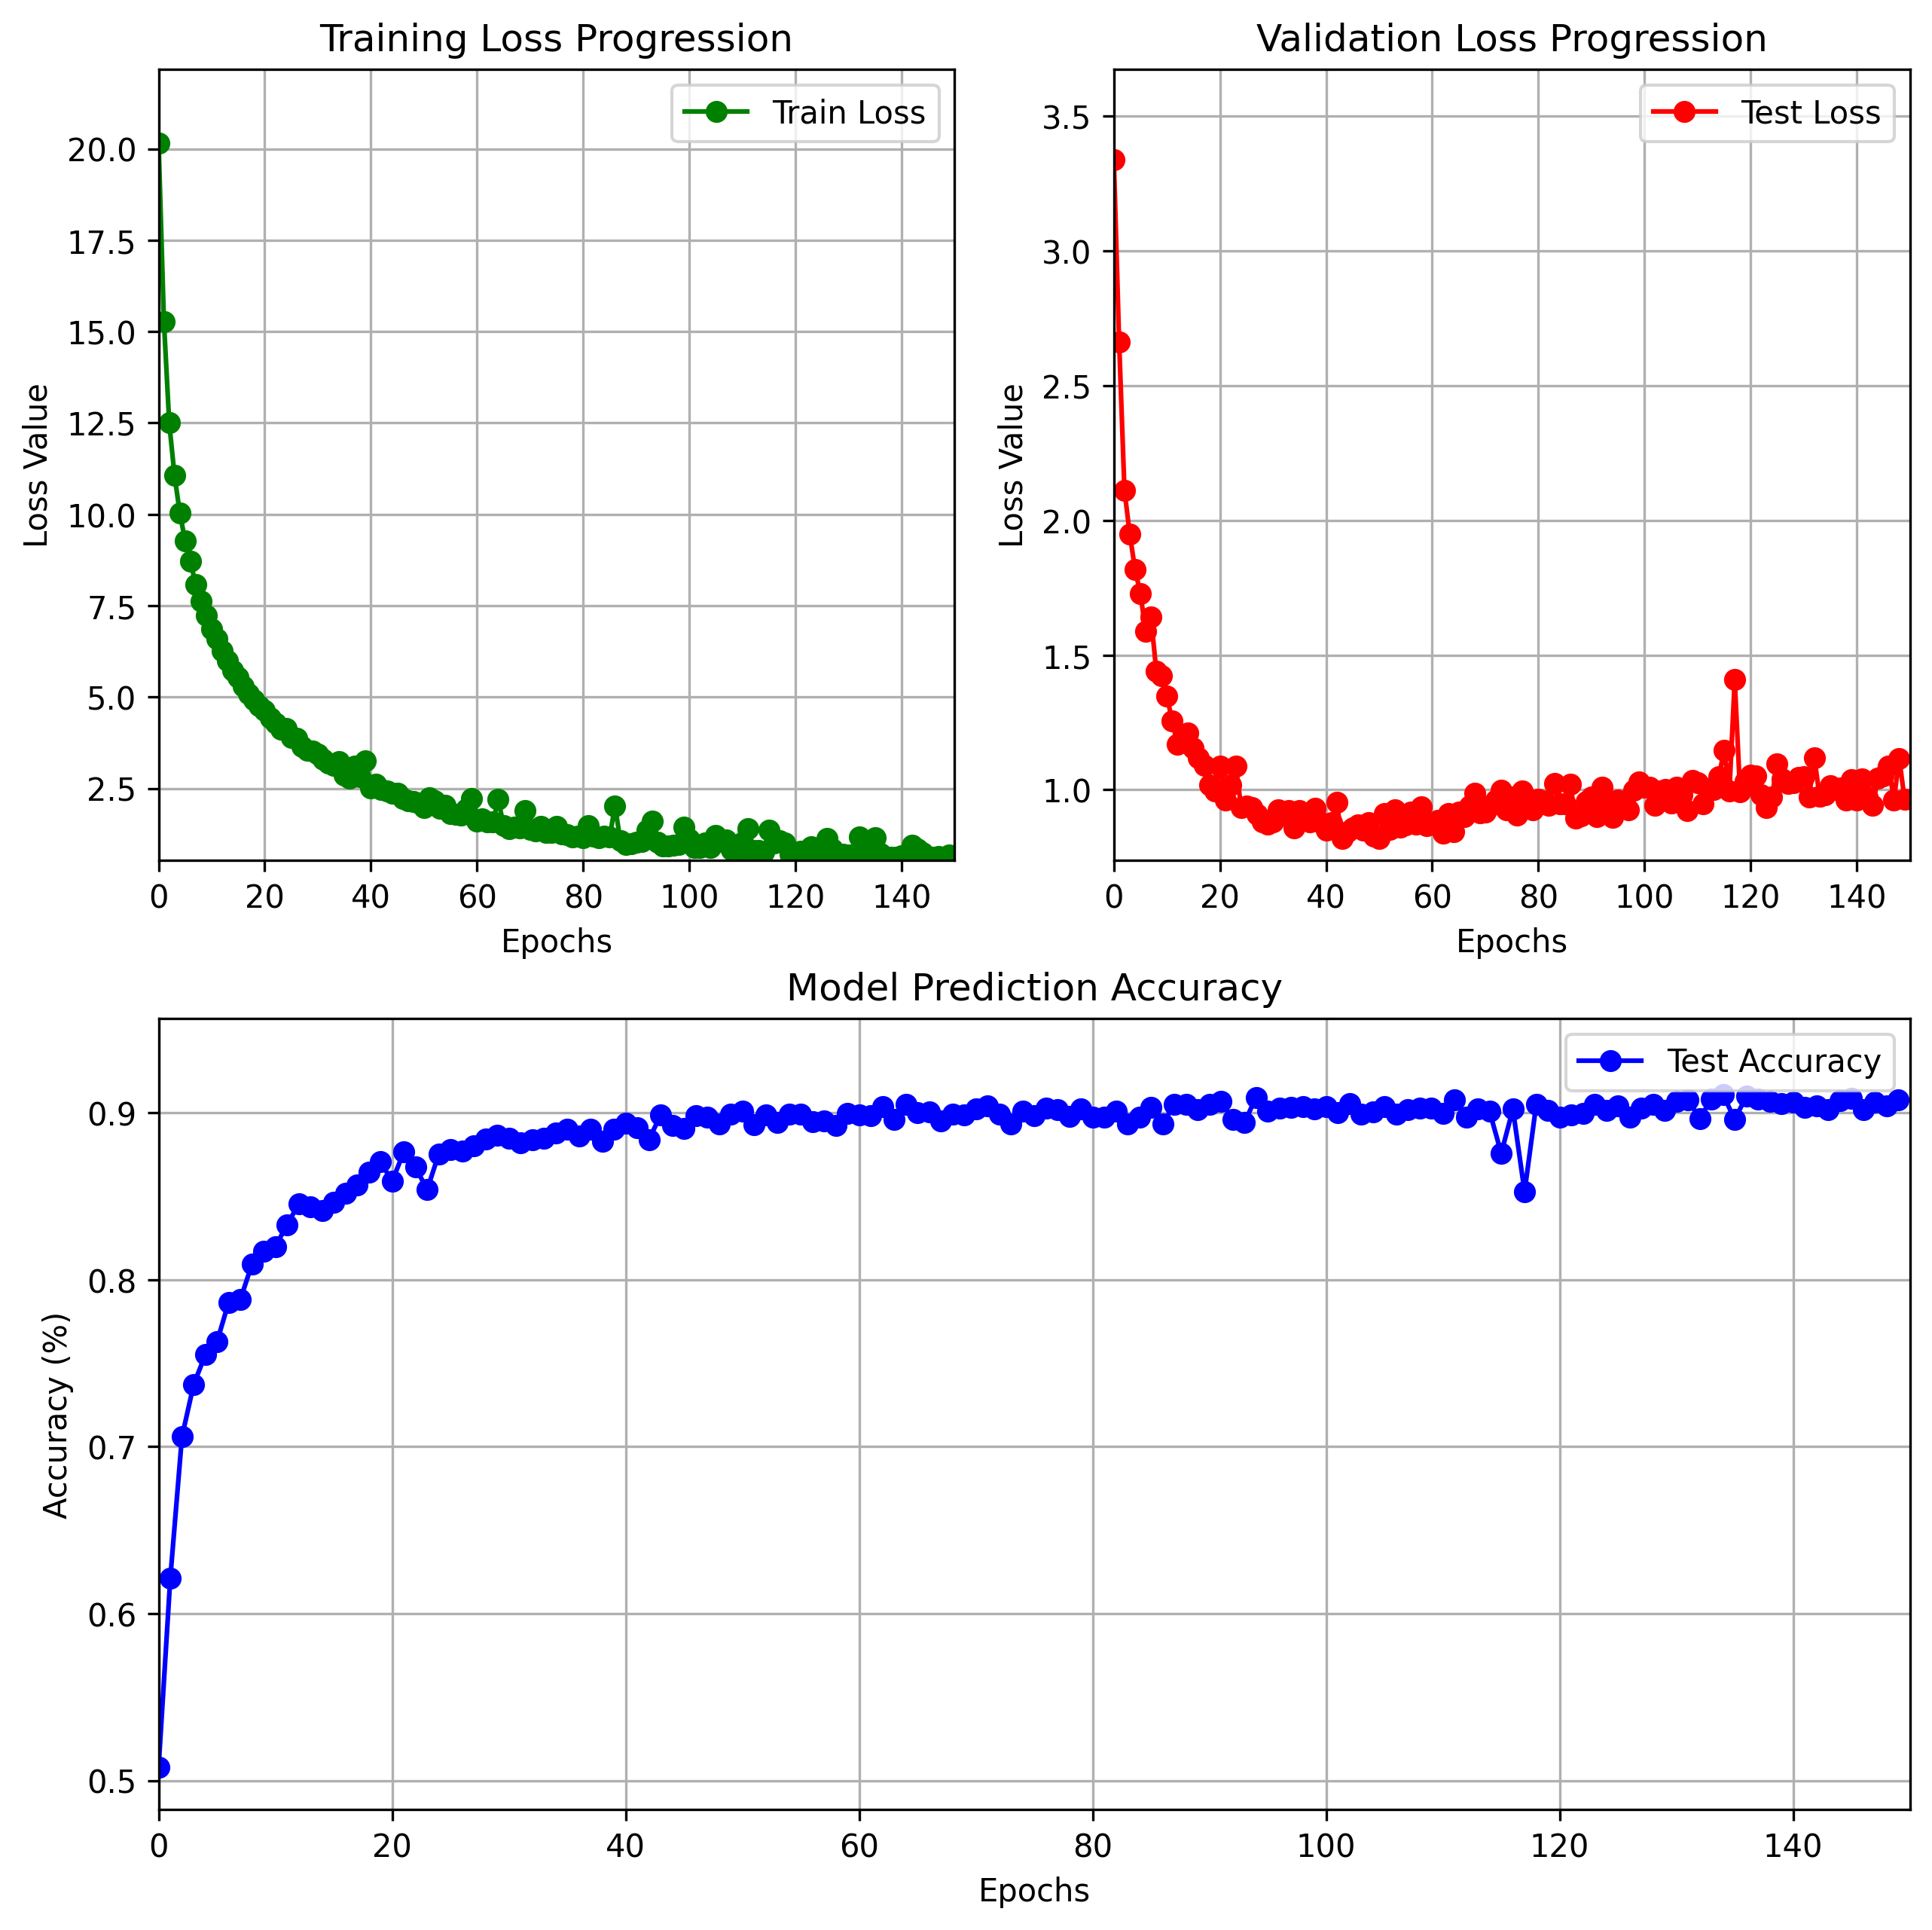
\includegraphics[width=0.3\textwidth]{fig/train_result_vgg16.png} % 设定图片宽度
  
  \caption{ ResNet18(left), ResNet50(middle), vgg16(right)} % 图片标题
  \label{fig:curve} % 图片标签,方便引用
\end{figure}
\noindent We can terpretate from the results:
\begin{itemize}
  \item deeper neural networks are more capable of learning picture pattern than lower ones
  \item we can see from the loss curves that, these 3 deep neural network do not grow as much as basline model in testing loss as epoch goes up: they are less likely to be overfitting than our baseline model, and hence get a higher testing accuracy: 92\%+.
  \item ResNets are better than vgg16 because of the skip connections between ResidualBlocks so the gradients propagate in a more stable manner.
  \item VGG16 aggressively reduces resolution via max-pooling (5 maxpooling layer, causing the receptive field to shrink to 1x1), causing severe spatial information loss in later layers. While ResNet preserves details through gradual downsampling.
\end{itemize}






\subs{3 Train and eval on MNIST dataset}
We decide to test 2 models in MNIST dataset: 1) Baseline model with BEST settings (setting 3: Adam+dropout after linear + batchnorm), 2) ResNet18. 
\textcolor{red}{Notice that MNIST's image has only 1 channel instead of 3, the extra data augmentation--Color jit will automatically idle: doing nothing to the figure}, an example of origianl image and image after transformed are like:

\begin{figure}[hbtp]
  \centering
  
  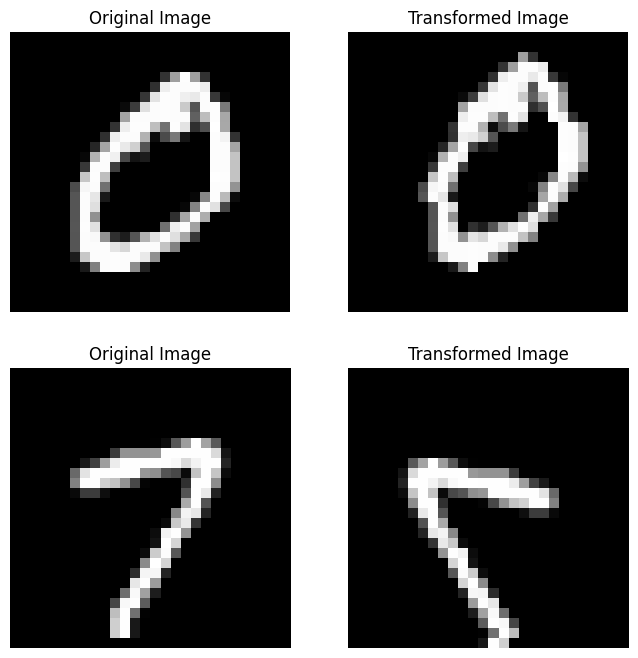
\includegraphics[width=0.4\textwidth]{fig/mnist.png} % 设定图片宽度
  
  \caption{MNIST image: original 0/7 (left coolumn), transformed 0/7 (right column)} % 图片标题
  \label{fig:curve} % 图片标签,方便引用
\end{figure}

\noindent Results are shown in Table 3 and Figure 8:
\noindent We can interprate from the result:
\begin{itemize}
  \item We can see diminishing returns of depth here:
  ResNet18's residual connections and deeper layers (18 layers) are designed to solve vanishing gradients and feature degradation in very deep networks (e.g., 50+ layers).
  
  For MNIST's shallow feature hierarchy, these mechanisms provide negligible benefits, as even simple CNN structures avoid gradient issues at this depth.
  \item The dataset's 60,000 training samples are sufficient to regularize both simple and moderately complex models, preventing overfitting. 
  ResNet18's parameters (~11M) are not excessively large relative to MNIST's size, unlike scenarios with smaller datasets (e.g., CIFAR-10 with 5k samples per class).
  \item MNIST's simplicity creates a "performance ceiling" where even modest models achieve near-perfect accuracy, rendering architectural refinements largely unnecessary. The observed parity underscores the importance of matching model complexity to task difficulty.
\end{itemize}

\begin{table}[htbp]
  \centering
  \caption{ModelSettings and Performance on cifar-10}
  \label{tab:model-compare}
  \begin{tabular}{|c|cc|} 
    \hline
    Model & BaseLine Best & ResNet18   \\
    \hline
    TestAcc & 99.35 & 99.50  \\
    \hline
  \end{tabular} 
\end{table}

\begin{figure}[H]
  \centering
  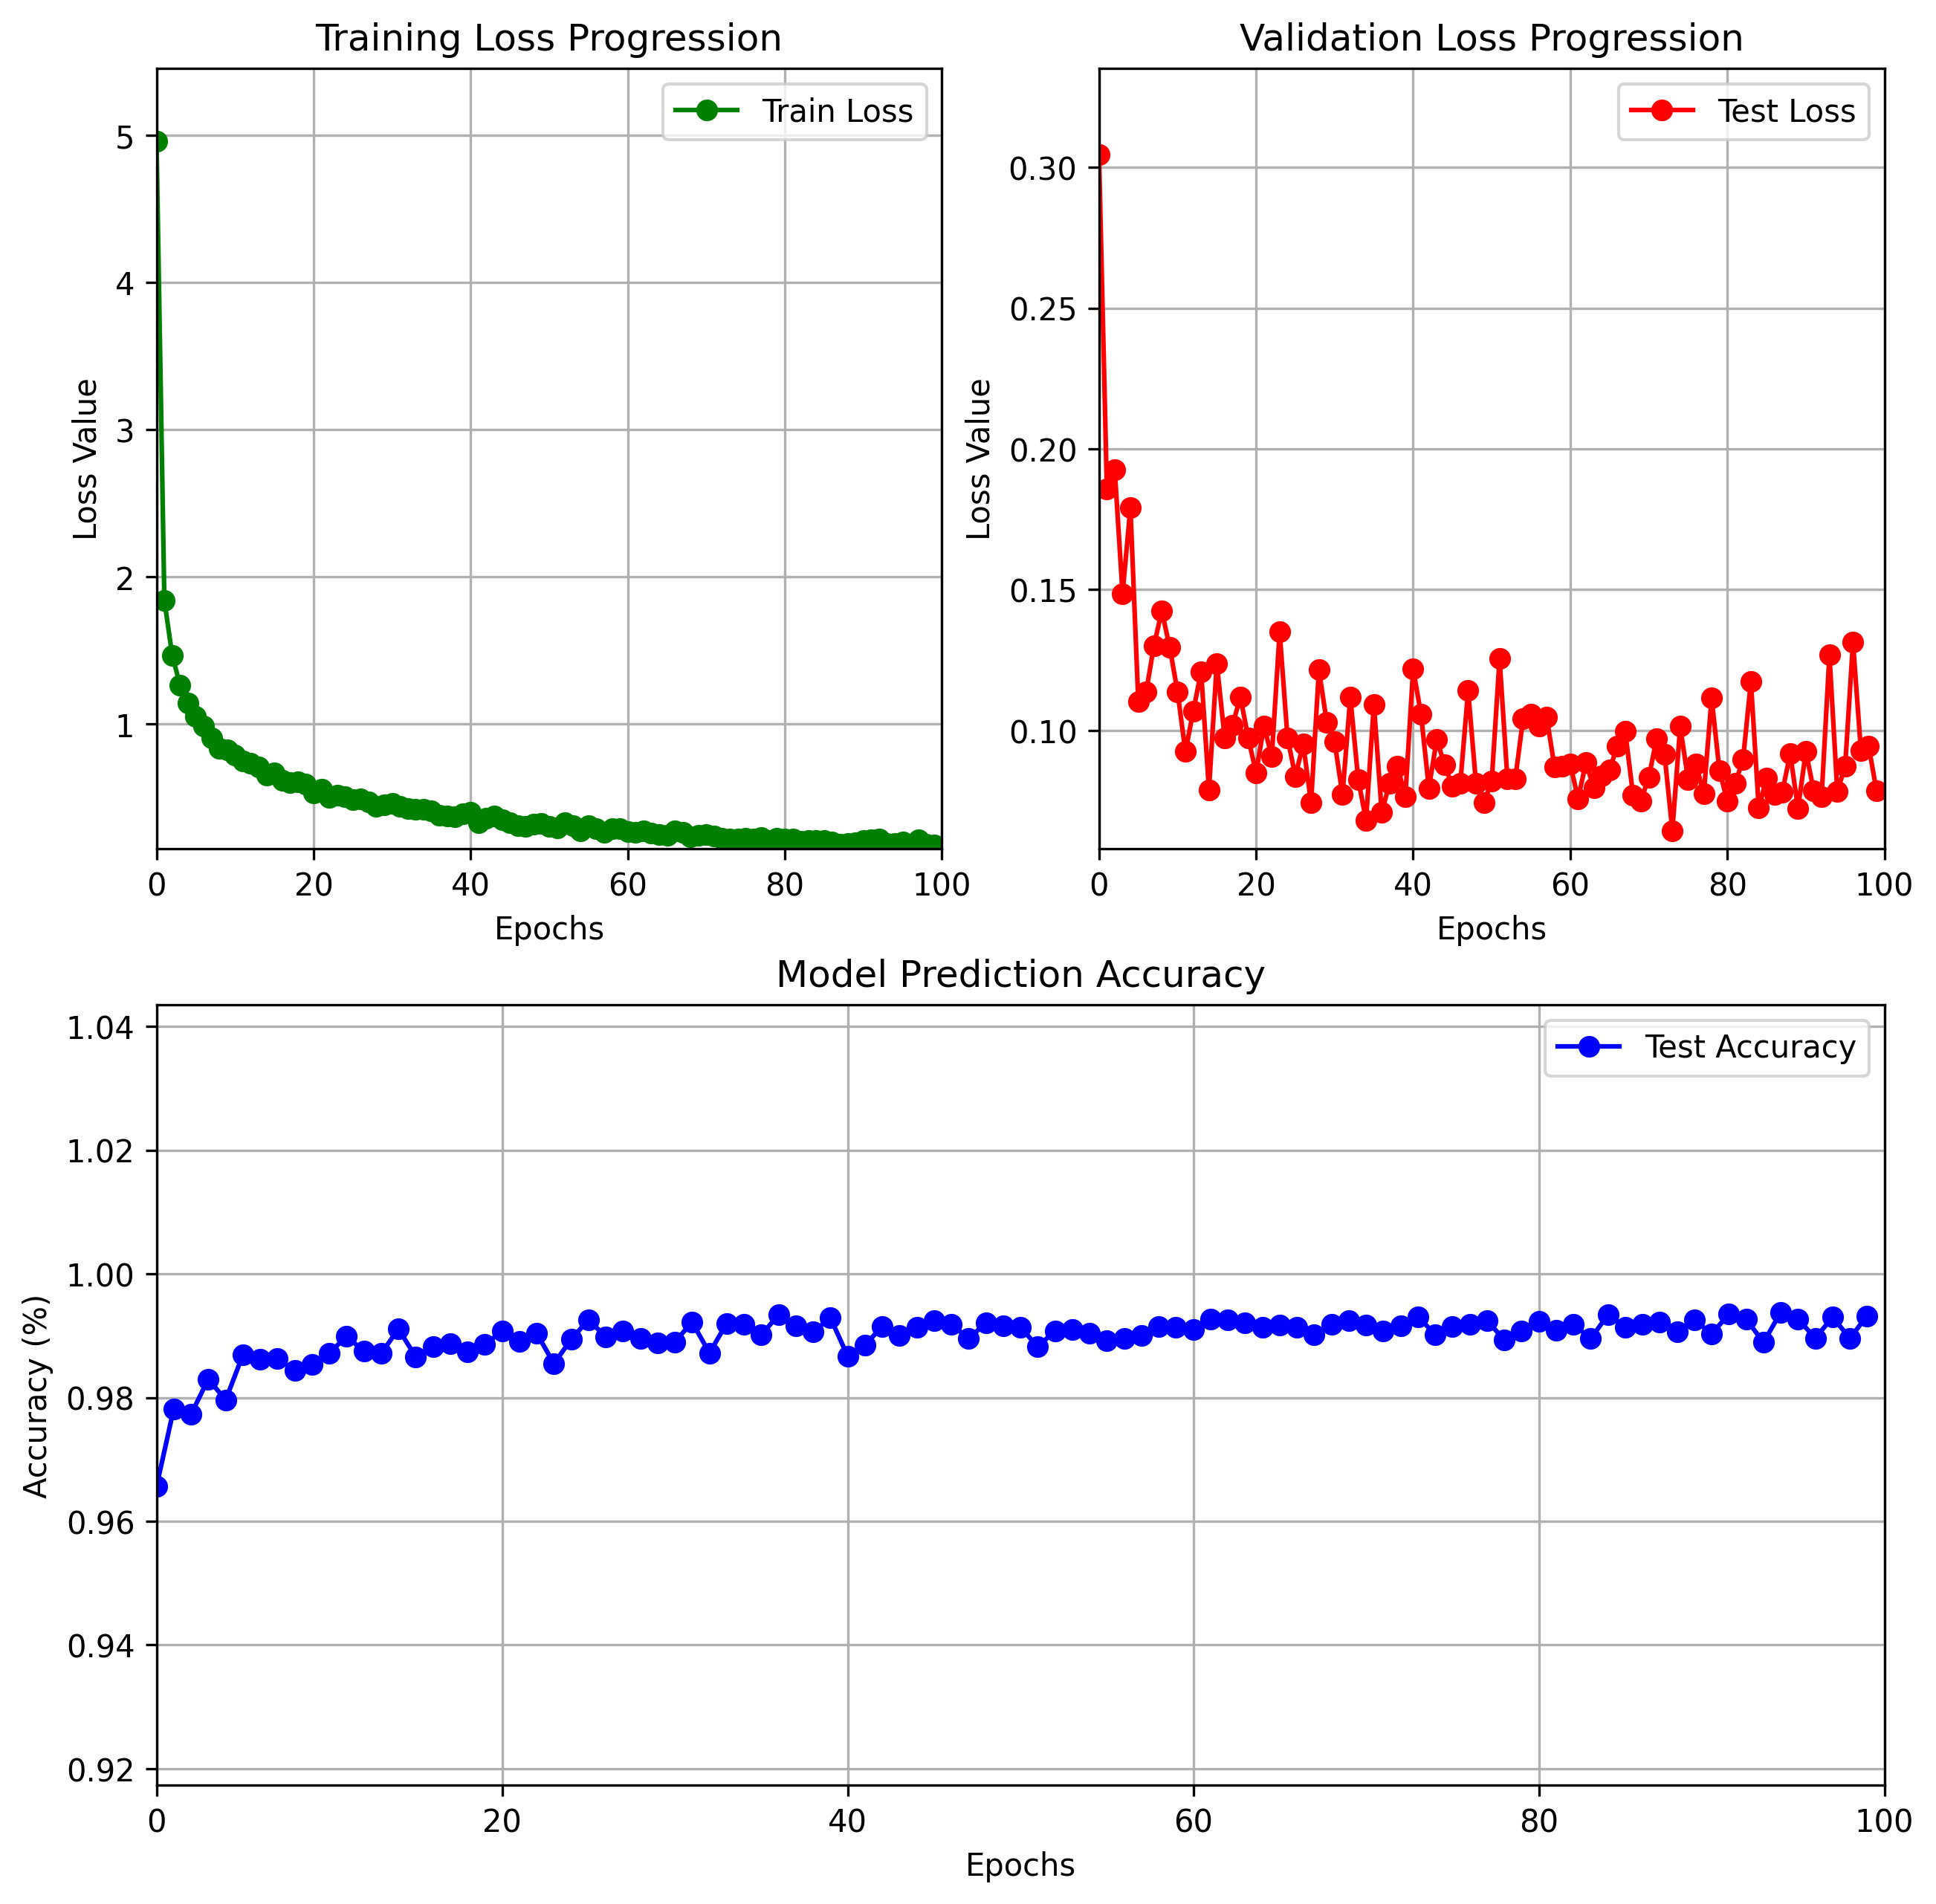
\includegraphics[width=0.45\textwidth]{fig/train_result_bsln_mnist.png} % 设定图片宽度
  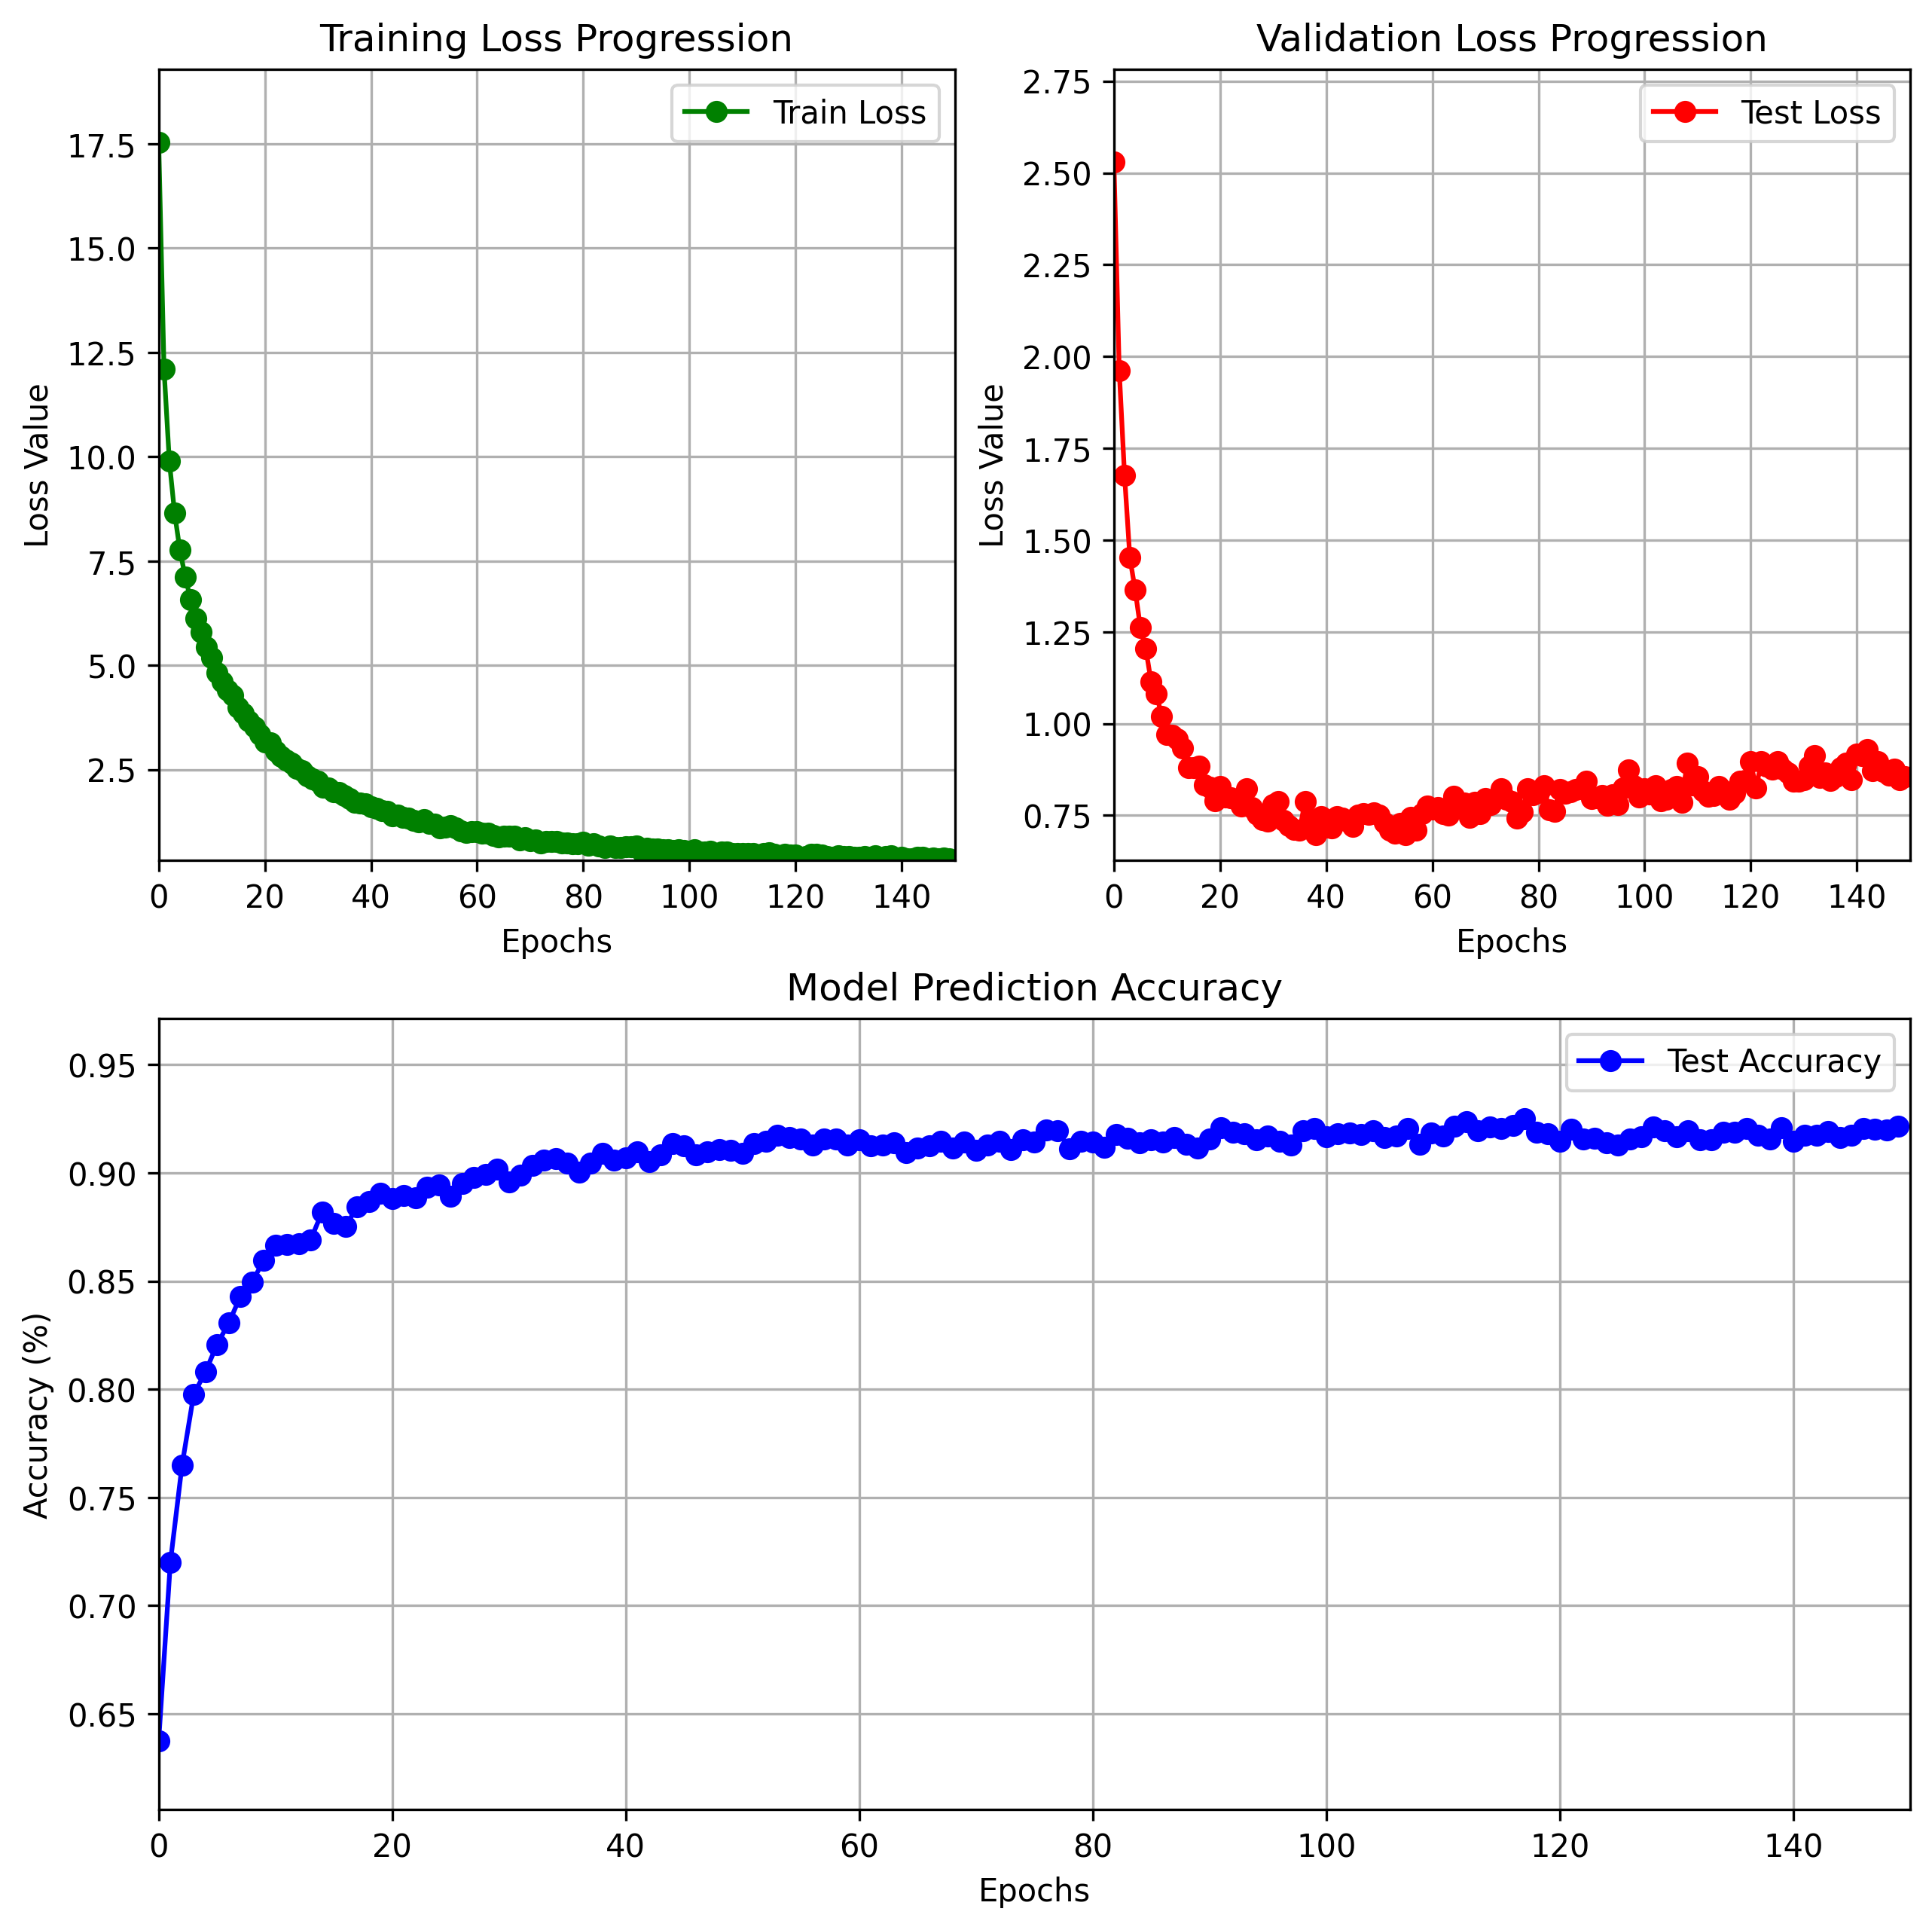
\includegraphics[width=0.45\textwidth]{fig/train_result_res18.png} % 设定图片宽度
  \caption{Basline(left), ResNet18(right) on MNIST} % 图片标题
  \label{fig:curve} % 图片标签,方便引用
\end{figure}



\subs{Interesting findings and reflections(What have i learnt)}
\noindent 1) I wasted significant amount of time tuning hyperparameters because the original training framework had messy dependencies between variables – adjusting a single parameter often required modifying multiple places. This ultimately drove me to encapsulate the entire workflow (data preprocessing, model selection, optimizer configuration, training loop, result saving, and visualization) into a massive main function, exposing only hyperparameters via an API.\\

\noindent 2) Avoid stucking all experiments into a single \texttt{.ipynb} file. If any error occurs midway (which is common due to discrepancies between the training environment and local debugging environment), all training results could be lost. Therefore, I chose to execute each experiment in separate files, even though this approach appears less organized.\\

\noindent 3) When constructing neural networks, one must consider the input image's channel nums. While using lazy-initialized layers like \texttt{nn.LazyConv2d} can automatically adapt to input channel dimensions, this approach introduces a limitation: you cannot calculate or print the model's total parameter count before feeding data to the model. Instead, you must first pass a dummy data batch to trigger lazy initialization, after which the layers will have initialized parameters.

\newpage
\secs{B. Build a Neural Network From Scratch}
\subs{AutoGrad: To Learn from the better}
When attempting to build a deep learning framework from scratch, I referenced numerous materials, including Example-Code-Part-B and PyTorch. However, PyTorch is an immensely large framework that integrates numerous heavily optimized modules. The implementation logic of most modules has become unrecognizable under massive speed and compatibility optimizations, which makes it akin to a "rocket science project" for a beginner. At least for me, it is not a good reference material.\\

In Example-Code-Part-B, the implementation of backpropagation relies on MANUALLY deriving gradients and writing them into .backward() methods, which are then called in a nested way to perform backward propagation when gradients are needed. This raised concerns for me: For more complex network architectures (e.g., ResidualBlock in ResNet), manual gradient derivation would be nearly impossible. Does this mean that after painstakingly "implementing" the simple functionalities required for the assignment, I still cannot gain much insight into the model DL framework (especially AutoGrad and Computing Graph), or to use these components to build more sophisticated networks?\\

This concern drove me to explore further, leading me to discover the Chainer framework. Its core innovation is automatic differentiation via the dynamic computational graph (Define-by-Run), which allows users to construct the computation graph on-the-fly during the forward propagation process then attain gradients automatically, rather than predefining a static structure. Chainer was the first framework to propose dynamic computational graphs and inspired PyTorch's design. However, Chainer's high complexity still made it unsuitable for a novice learner.\\

I then discovered the book Building Deep Learning Frame, which introduces a framework called DeZero—a simplified version of Chainer. It is sufficiently complex and flexible, yet not overly daunting for learners. The book provides the complete source code for DeZero, but simply copying the code would not have benefited me. Since I started this project early (immediately after the assignment was released), I spent two full weeks studying every line of DeZero's code character by character. I abandoned the author’s original implementation of the Conv2d module and reimplemented it from scratch, and I independently implemented FocalLoss module, which were not provided by the author, as tests to verify my understanding. All of this was made possible by the concepts of automatic differentiation and dynamic computational graphs, freeing me from the agony of manual gradient derivation and debugging, and preparing me to build complex deep networks like ResNet18/50 in the future.

\subs{File Structure of the self-made framework: How to run}
\begin{itemize}
  \item All necessary codes for Task B are packed in \texttt{./dezero-master}
  \item \texttt{./dezero-master/dezero} contains all source code of the self-made framework, it can be imported like a normal python packages just like pytorch.
  \item \texttt{./dezero-master/dezero/dezero\_bsln.ipynb \& dezero\_res18.ipynb} is the training files, push it to kaggle like before to start training. \textcolor{red}{All training results/weights, including visualization of train/test loss and test accuracy will be saved to /kaggle/output automatically.}
\end{itemize}
\noindent 
\textbf{The core of my framework is Define-by-Run AutoGrad, it builds connections between variables for later back-propagation when doing calculation.} The DeZero module is composed of a series of \texttt{.py} files, which can be imported like a standard Python package using \texttt{import}. Below I will outline the module's file structures and map the assignment-required functionalities to their corresponding implementations position. For certain noteworthy implementation approaches, I will briefly discuss them here.

\begin{lstlisting}[language=python]

  dezero-master: .
  │  core.py --------# base class: Function and Variable(a torch.tensor like data structure), core modules for define-by run AutoGrad
  │  core_copy_beforeCuPY.py --------# ignore, testing module
  │  core_simple.py --------# ignore, testing module
  │  cuda.py --------# cupy adaptation
  │  dataloaders.py
  │  datasets.py
  │  functions.py --------# Sigmoid/LeakyReLU/SELU/Dropout/FocalLoss
  │  functions_conv.py --------#conv modules: F.Conv2dV function
  │  layers.py --------# Linear/Conv2dV(Conv2d)/BatchNorm(BatchNorm2d)
  │  models.py --------# C5L3/vgg16/ResNet18/50
  │  optimizers.py --------# SGD/Adam
  │  utils.py
  │  __init__.py
\end{lstlisting}
\vspace{5mm}

\subs{1. Implementations}
\noindent My implementation codes path:\\
\begin{itemize}
  \item[a)] \textbf{Sigmoid}: ../dezero-master/dezero/functions.py - line 457
  \item[b)] \textbf{LeakyReLU}: ../dezero-master/dezero/functions.py - line 509
  \item[c)] \textbf{SELU}: ../dezero-master/dezero/functions.py - line 670
  \item[d)] \textbf{Linear}: ../dezero-master/dezero/layers.py - line 118
  \item[e)] \textbf{Conv2d/Conv2dV}: ../dezero-master/dezero/layers.py - line 221, the standard conv2d implementation is complicated, i also wrote a new one (named Conv2dV) with im2col in forward and col2im in backward, almost as fast as the original one. \textcolor{red}{And the reproduction of the results from task A using my framework adopts Conv2dV as convolution layers.}
  \item[f)] \textbf{Dropout}: ../dezero-master/dezero/functions.py - line 691
  \item[g)] \textbf{BatchNorm(BatchNorm2d)}: ../dezero-master/dezero/layers.py - line 311, automatically detect \texttt{num\_features}, so no need to add this config
  \item[h)] \textbf{SigmoidFocalLoss\_manual/SigmoidFocalLoss\_simple}: ../dezero-master/dezero/functions.py - Line 570, 2 ways of implementation: 
  1) manually: \texttt{SigmoidFolcaLoss} implementation adopt \texttt{.forward(), .backward()}, which will be slightly faster; 2) automatically: \texttt{SigmoidFocalLoss\_simple} only calculate the forward procedure, \textcolor{red}{but the backward calculation can be done automatically via AutoGrad}
  \item[i)] \textbf{SGD}: ../dezero-master/dezero/optimizers.py - line 38
  \item[j)] \textbf{Adam}: ../dezero-master/dezero/optimizers.py - line 84   
\end{itemize}
\vspace{5mm}
\subs{1.2 Testing implementations that not be used}
\noindent Since \texttt{LeakyReLU, SELU, SigmoidFocalLoss} will not be used by my reproduction, we first test them and compare the results to \texttt{torch.nn.functions}'s implementation to see if they actually do the right things:
\textcolor{red}{all test codes are packed in \texttt{../dezero-master/DeZero\_test\_notes.ipynb}}

\begin{lstlisting}[language=python]
  # test self-made framework's sigmoid focal loss
  from imp import reload
  from dezero import Variable
  import dezero.functions as F
  reload(F)
  import numpy as np

  # input a random variable into  sigmoid focalloss
  x = Variable(np.array([1.0, -3.0,2], dtype=np.float32))
  target = Variable(np.array([0.0, 1.0, 0.0], dtype=np.float32))

  # cal focal loss (forward test)
  loss = F.sigmoid_focal_loss_manual(x, target, alpha=0.25, gamma=3)
  print("Loss:", loss.data) 
  # cal gradient (backward test)
  x.cleargrad()
  loss.backward()
  print(x.grad)

  # loss and gradients:
  >>> Loss: [0.7112133]
  >>> gradients: variable([ 0.17490506 -0.099857    0.28040347])


  # verify using torchvision.ops.sigmoid_focal_loss
  from torchvision.ops import sigmoid_focal_loss as focal
  import torch

  x = torch.tensor(np.array([1.0, -3.0, 2], dtype=np.float32), requires_grad=True)
  target = torch.tensor(np.array([0.0, 1.0, 0.0], dtype=np.float32), requires_grad=False)

  loss_torch = focal(x, target, alpha = 0.25, gamma = 3,reduction='mean')
  print("loss(torch):", loss_torch)

  loss_torch.backward()
  print("gradients(torch):",x.grad)

  >>> loss(torch): tensor(0.7112, grad_fn=<MeanBackward0>)
  >>> gradients(torch): tensor([ 0.1749, -0.0999,  0.2804])
\end{lstlisting}

\begin{lstlisting}[language=python]
  # self-made framework SELU test
  import dezero.functions as F
  from imp import reload
  reload(F)
  from dezero import Variable
  import torch
  import numpy as np

  x = Variable(np.array([1.0, -3.0,2.0, 5], dtype=np.float32))
  x_np = np.array([1.0, -3.0,2])
  y = F.sum(F.selu(x))
  y.cleargrad()
  y.backward()
  print("loss:", y)
  print("grads:", x.grad)

  >>> loss: variable(6.7350397)
  >>> grads: variable([1.0507009873554805 variable(0.08753060945898154) 1.0507009873554805
  1.0507009873554805])

  # verify using torch.nn.functional.selu
  x_t = torch.tensor(np.array([1.0, -3.0, 2.0, 5]), requires_grad = True,  dtype = torch.float32)
  
  y_t = torch.nn.functional.selu(x_t).sum()
  y_t.backward()
  print("loss(torch): ",y_t)
  print("grads(torch): ", x_t.grad)

  >>> loss(torch):  tensor(6.7350, grad_fn=<SumBackward0>)
  >>> grads(torch):  tensor([1.0507, 0.0875, 1.0507, 1.0507])
\end{lstlisting}

\begin{lstlisting}[language=python]
  # self-made framework's leaky relu test
  x = Variable(np.array([1.0, -3.0,2.0, 5], dtype=np.float32))
  y = F.sum(F.leaky_relu(x))
  y.cleargrad()
  y.backward()
  print("activation: ",y)
  print("grad: ", x.grad)
  
  >>> activation:  variable(7.9700003)
  >>> grad:  variable([1.   0.01 1.   1.  ])

  # verify with torch.nn.functional.leaky_rely 
  x_t = torch.tensor(np.array([1.0, -3.0, 2.0, 5]), requires_grad = True,  dtype = torch.float32)
  y_t = torch.nn.functional.leaky_relu(x_t,negative_slope=0.01).sum()
  y_t.backward()
  print("activation(torch): ", y_t)
  print("grads(torch): ", x_t.grad)

  >>> activation(torch):  tensor(7.9700, grad_fn=<SumBackward0>)
  >>> grads(torch):  tensor([1.0000, 0.0100, 1.0000, 1.0000])
\end{lstlisting}

\subs{1.3 Model structures under self-made framework}
\noindent\textcolor{blue}{Check models file at: ../dezero-master/dezero/models.py}. Here is an example of \texttt{Baseline} model under self-made:
\begin{lstlisting}[language=python]
  # C5L3, ignore below C5L4, wrong name
  class C5L4(Model):
      def __init__(self):
          super().__init__()
          self.conv1 = L.Conv2d(128,kernel_size=3, stride=1, pad=1)
          self.bn1 = L.BatchNorm2d()
  
          self.conv2 = L.Conv2d(256,kernel_size=3, stride=1, pad=1)
          self.bn2 = L.BatchNorm2d()
  
          self.conv3 = L.Conv2d(512,kernel_size=3, stride=1, pad=1)
          self.bn3 = L.BatchNorm2d()
  
          self.conv4 = L.Conv2d(512,kernel_size=3, stride=1, pad=1)
          self.bn4 = L.BatchNorm2d()
  
          self.conv5 = L.Conv2d(256,kernel_size=3, stride=1, pad=1)
          self.bn5 = L.BatchNorm2d()
  
          self.fc1 = L.Linear(512)
          self.fc2 = L.Linear(256)
          self.fc3 = L.Linear(128)
          self.fc4 = L.Linear(10)
      def forward(self, x):
          x = F.relu(self.bn1(self.conv1(x)))
          x = F.pooling(x, 2, 2)
          x = F.relu(self.bn2(self.conv2(x)))
          x = F.relu(self.bn3(self.conv3(x)))
          x = F.relu(self.bn4(self.conv4(x)))
          x = F.relu(self.bn5(self.conv5(x)))
          x = F.pooling(x, 2, 2)
  
          # flatten, x.shape[0] is N(batchsize)
          x = F.reshape(x, (x.shape[0], -1))
          # print(x.shape)
          x = F.dropout(F.relu(self.fc1(x)), dropout_ratio=0.3)
          x = F.dropout(F.relu(self.fc2(x)), dropout_ratio=0.3)
          x = F.dropout(F.relu(self.fc3(x)), dropout_ratio=0.3)
          x = self.fc4(x)
          return x
\end{lstlisting}

\secs{2. Reproducing Task A on MNIST}



\begin{table}[htbp]
  \centering
  \caption{Reproducing Task A on MNIST using self-made framework}
  \label{tab:model-compare}
  \begin{tabular}{|c|cc|} 
    \hline
    Model & BaseLine Best & ResNet18   \\
    \hline
    TestAcc(self-made) & 98.972 & 98.903  \\
    TestAcc(torch) & 99.35 & 99.50  \\
    \hline
  \end{tabular} 
\end{table}

\begin{figure}[H]
  \centering
  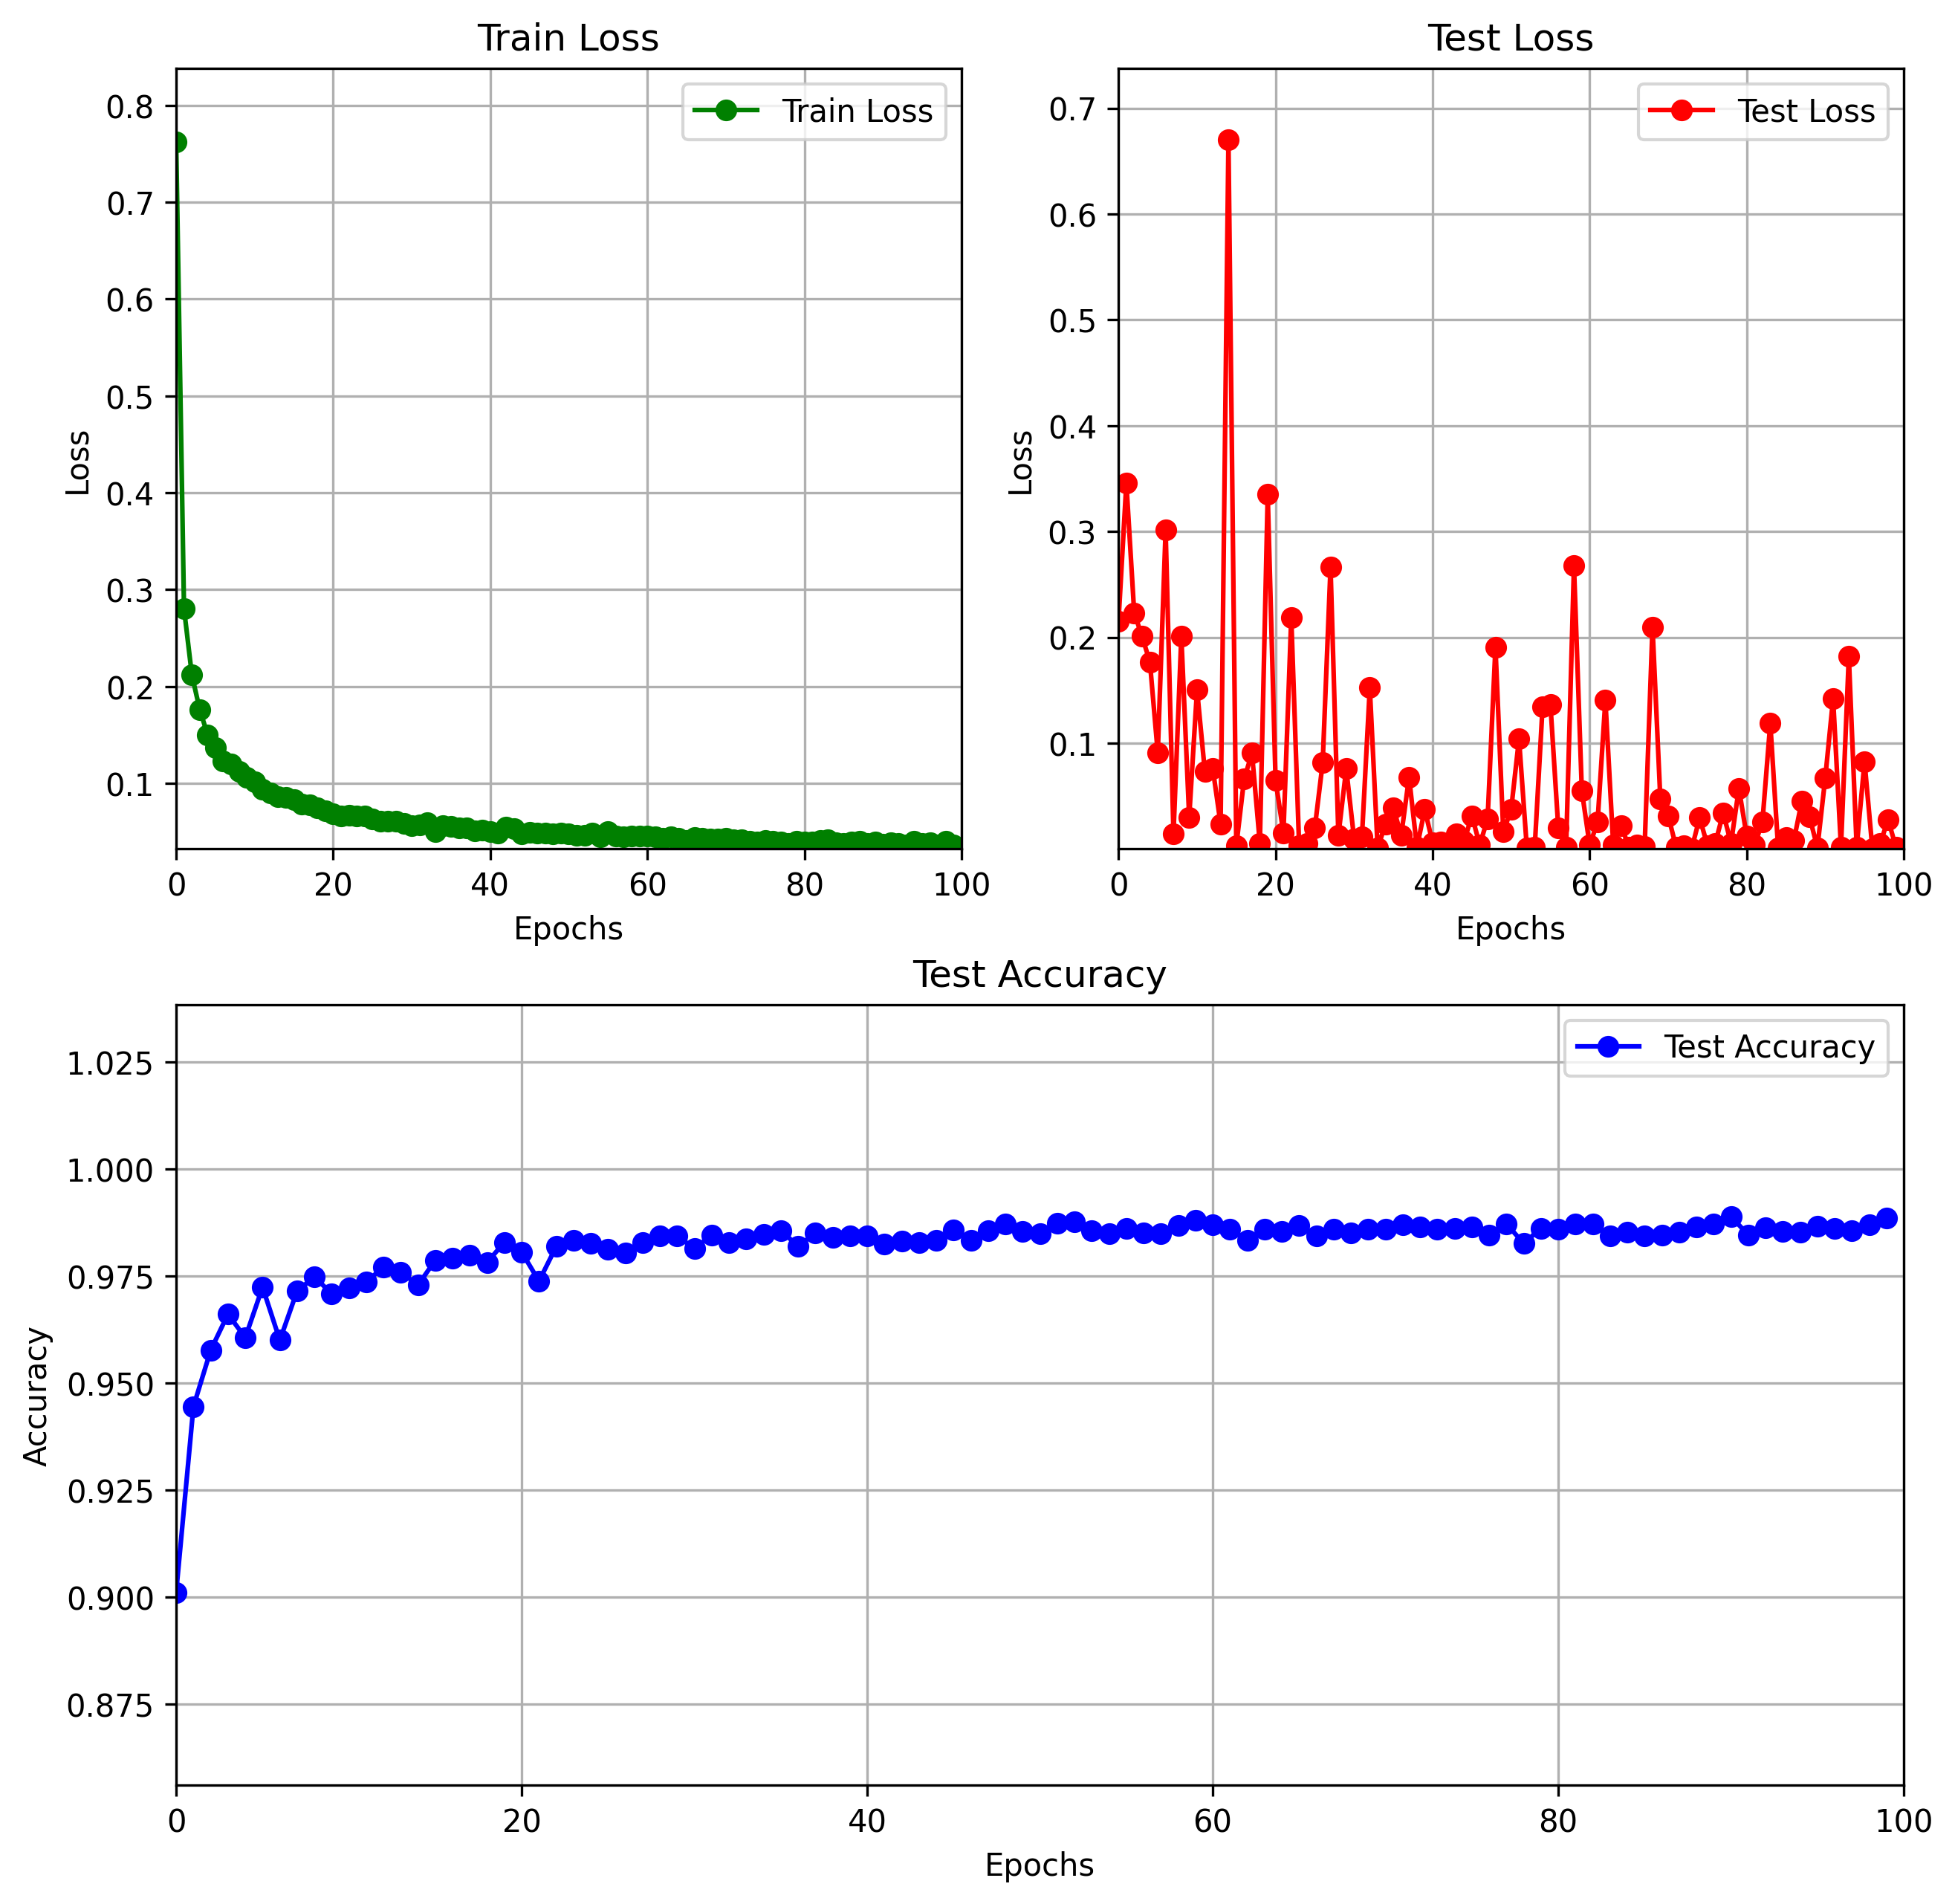
\includegraphics[width=0.45\textwidth]{fig/train_result_dezero_bsln.png} % 设定图片宽度
  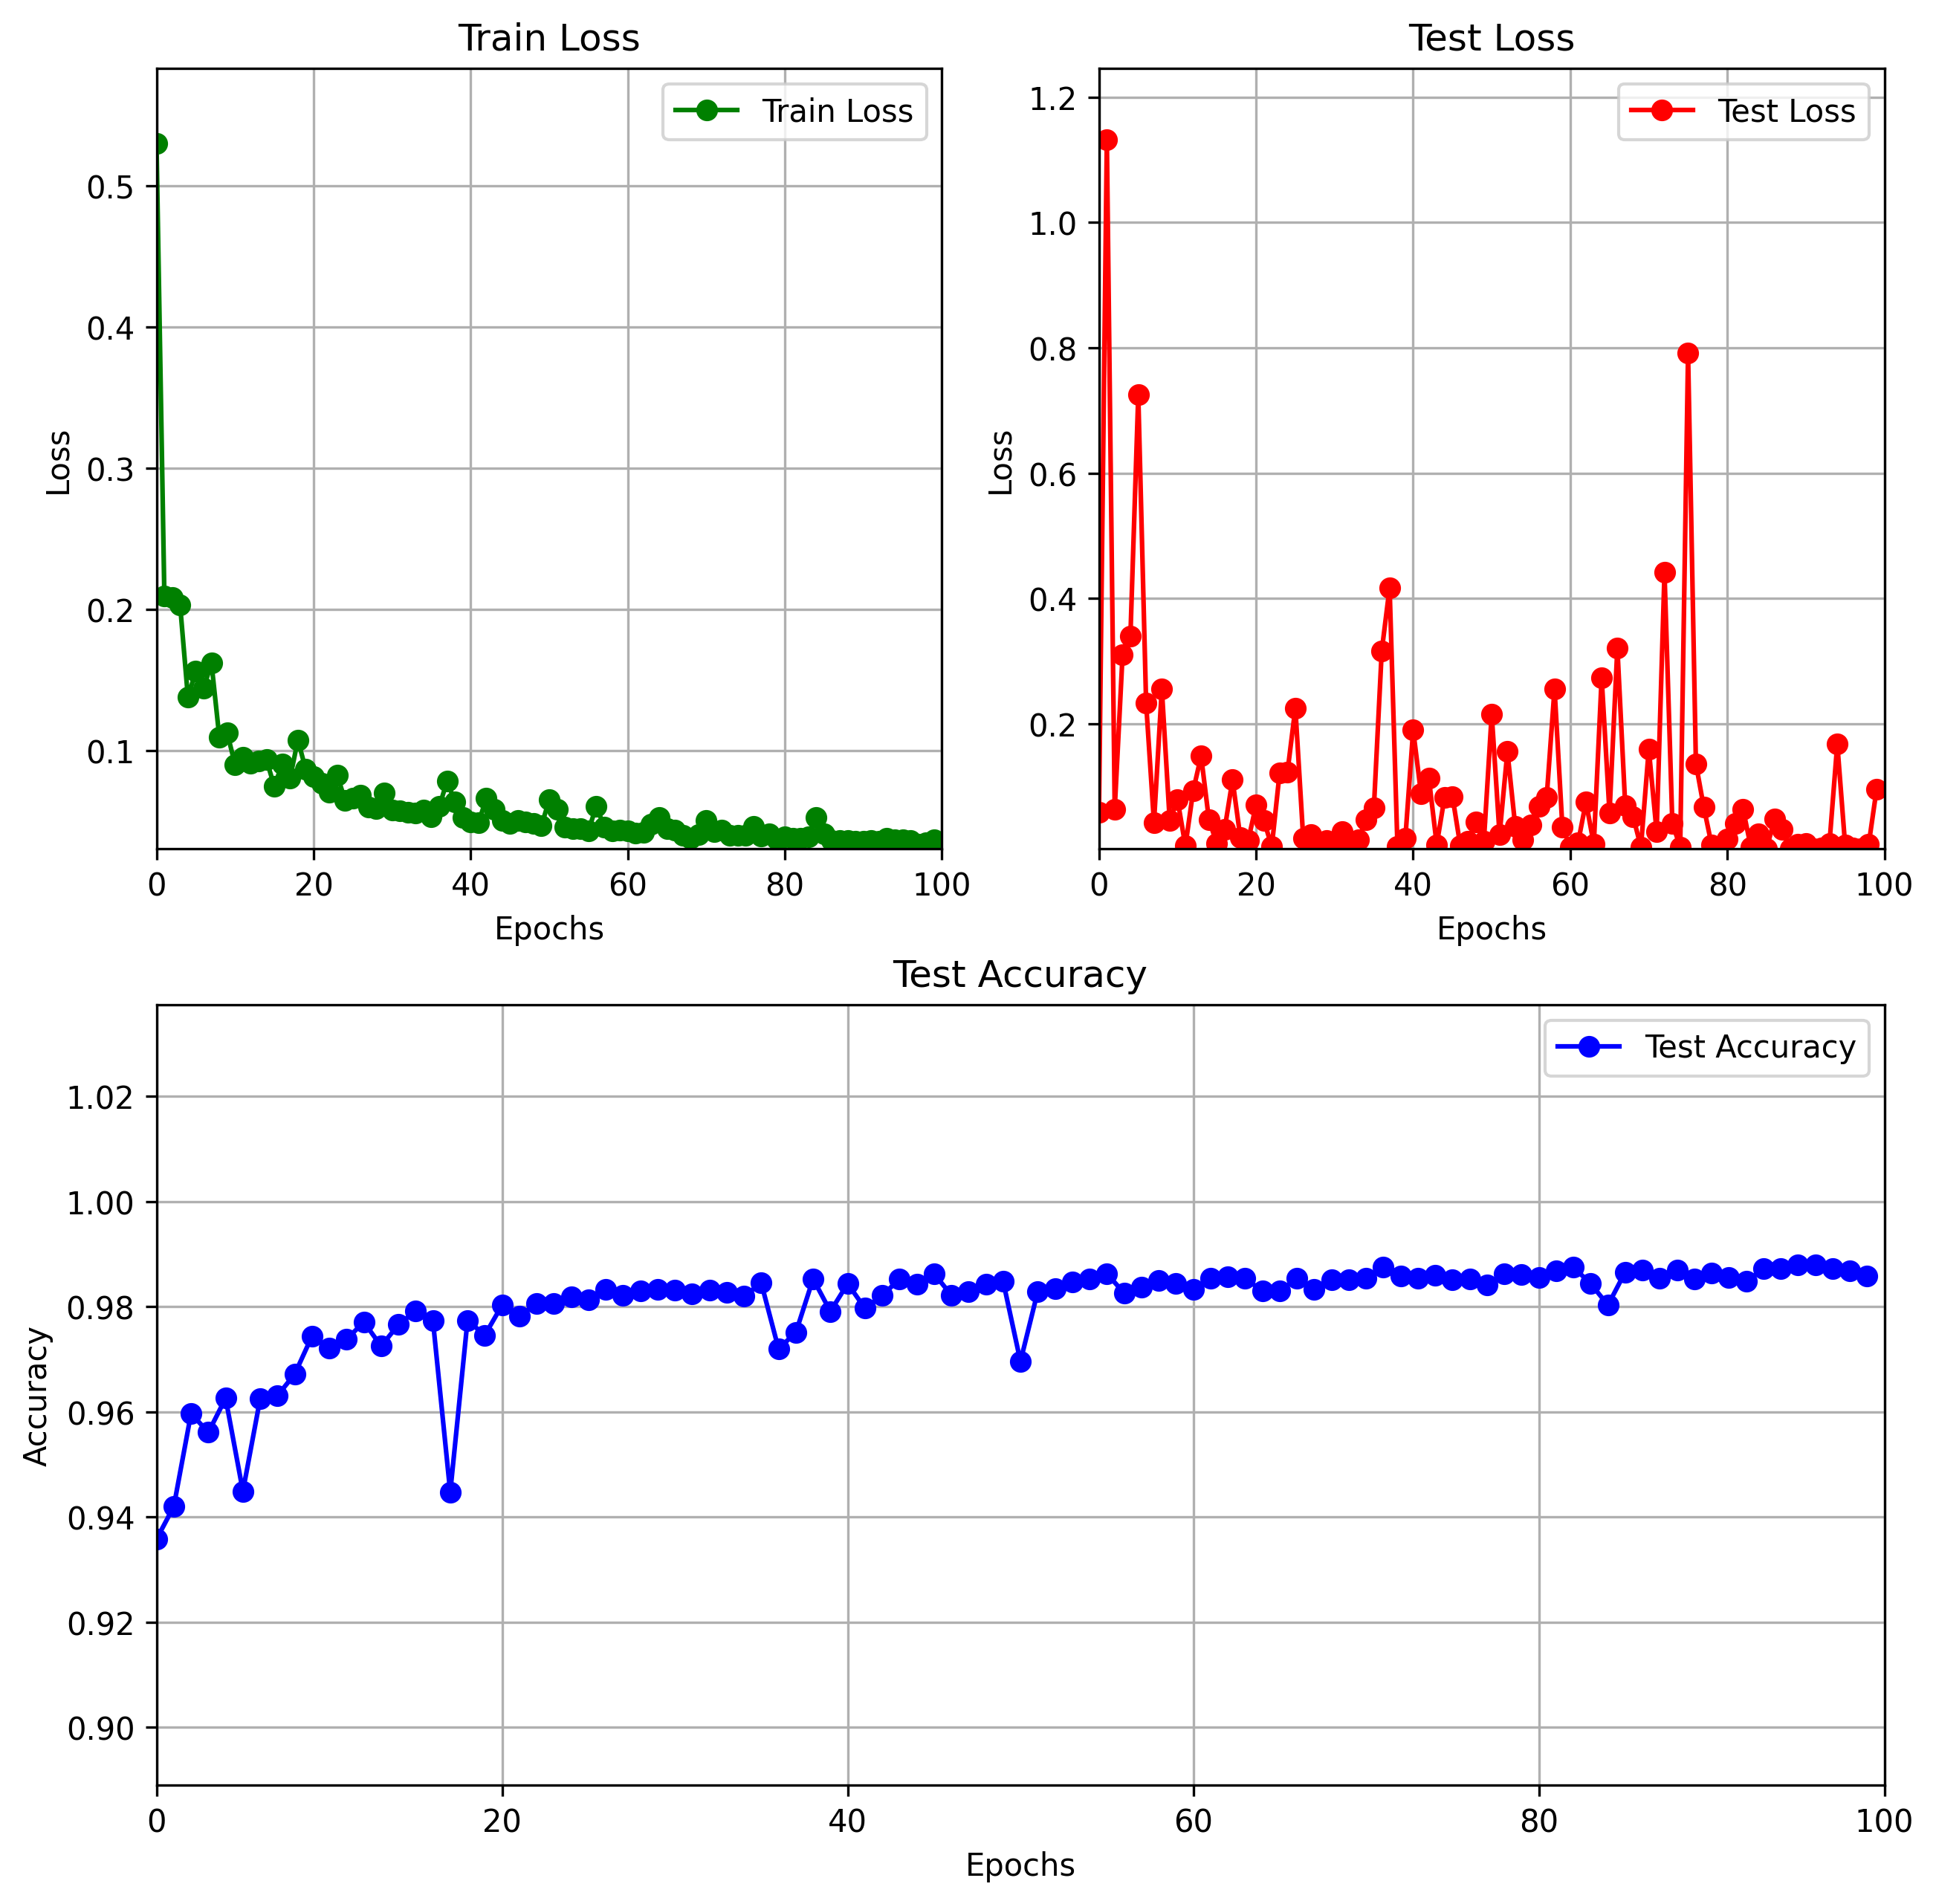
\includegraphics[width=0.45\textwidth]{fig/train_result_dezero_res18.png} % 设定图片宽度
  \caption{Basline(left), ResNet18(right) on MNIST using self-made framework} % 图片标题
  \label{fig:curve} % 图片标签,方便引用
\end{figure}

\begin{figure}[H]
  \centering
  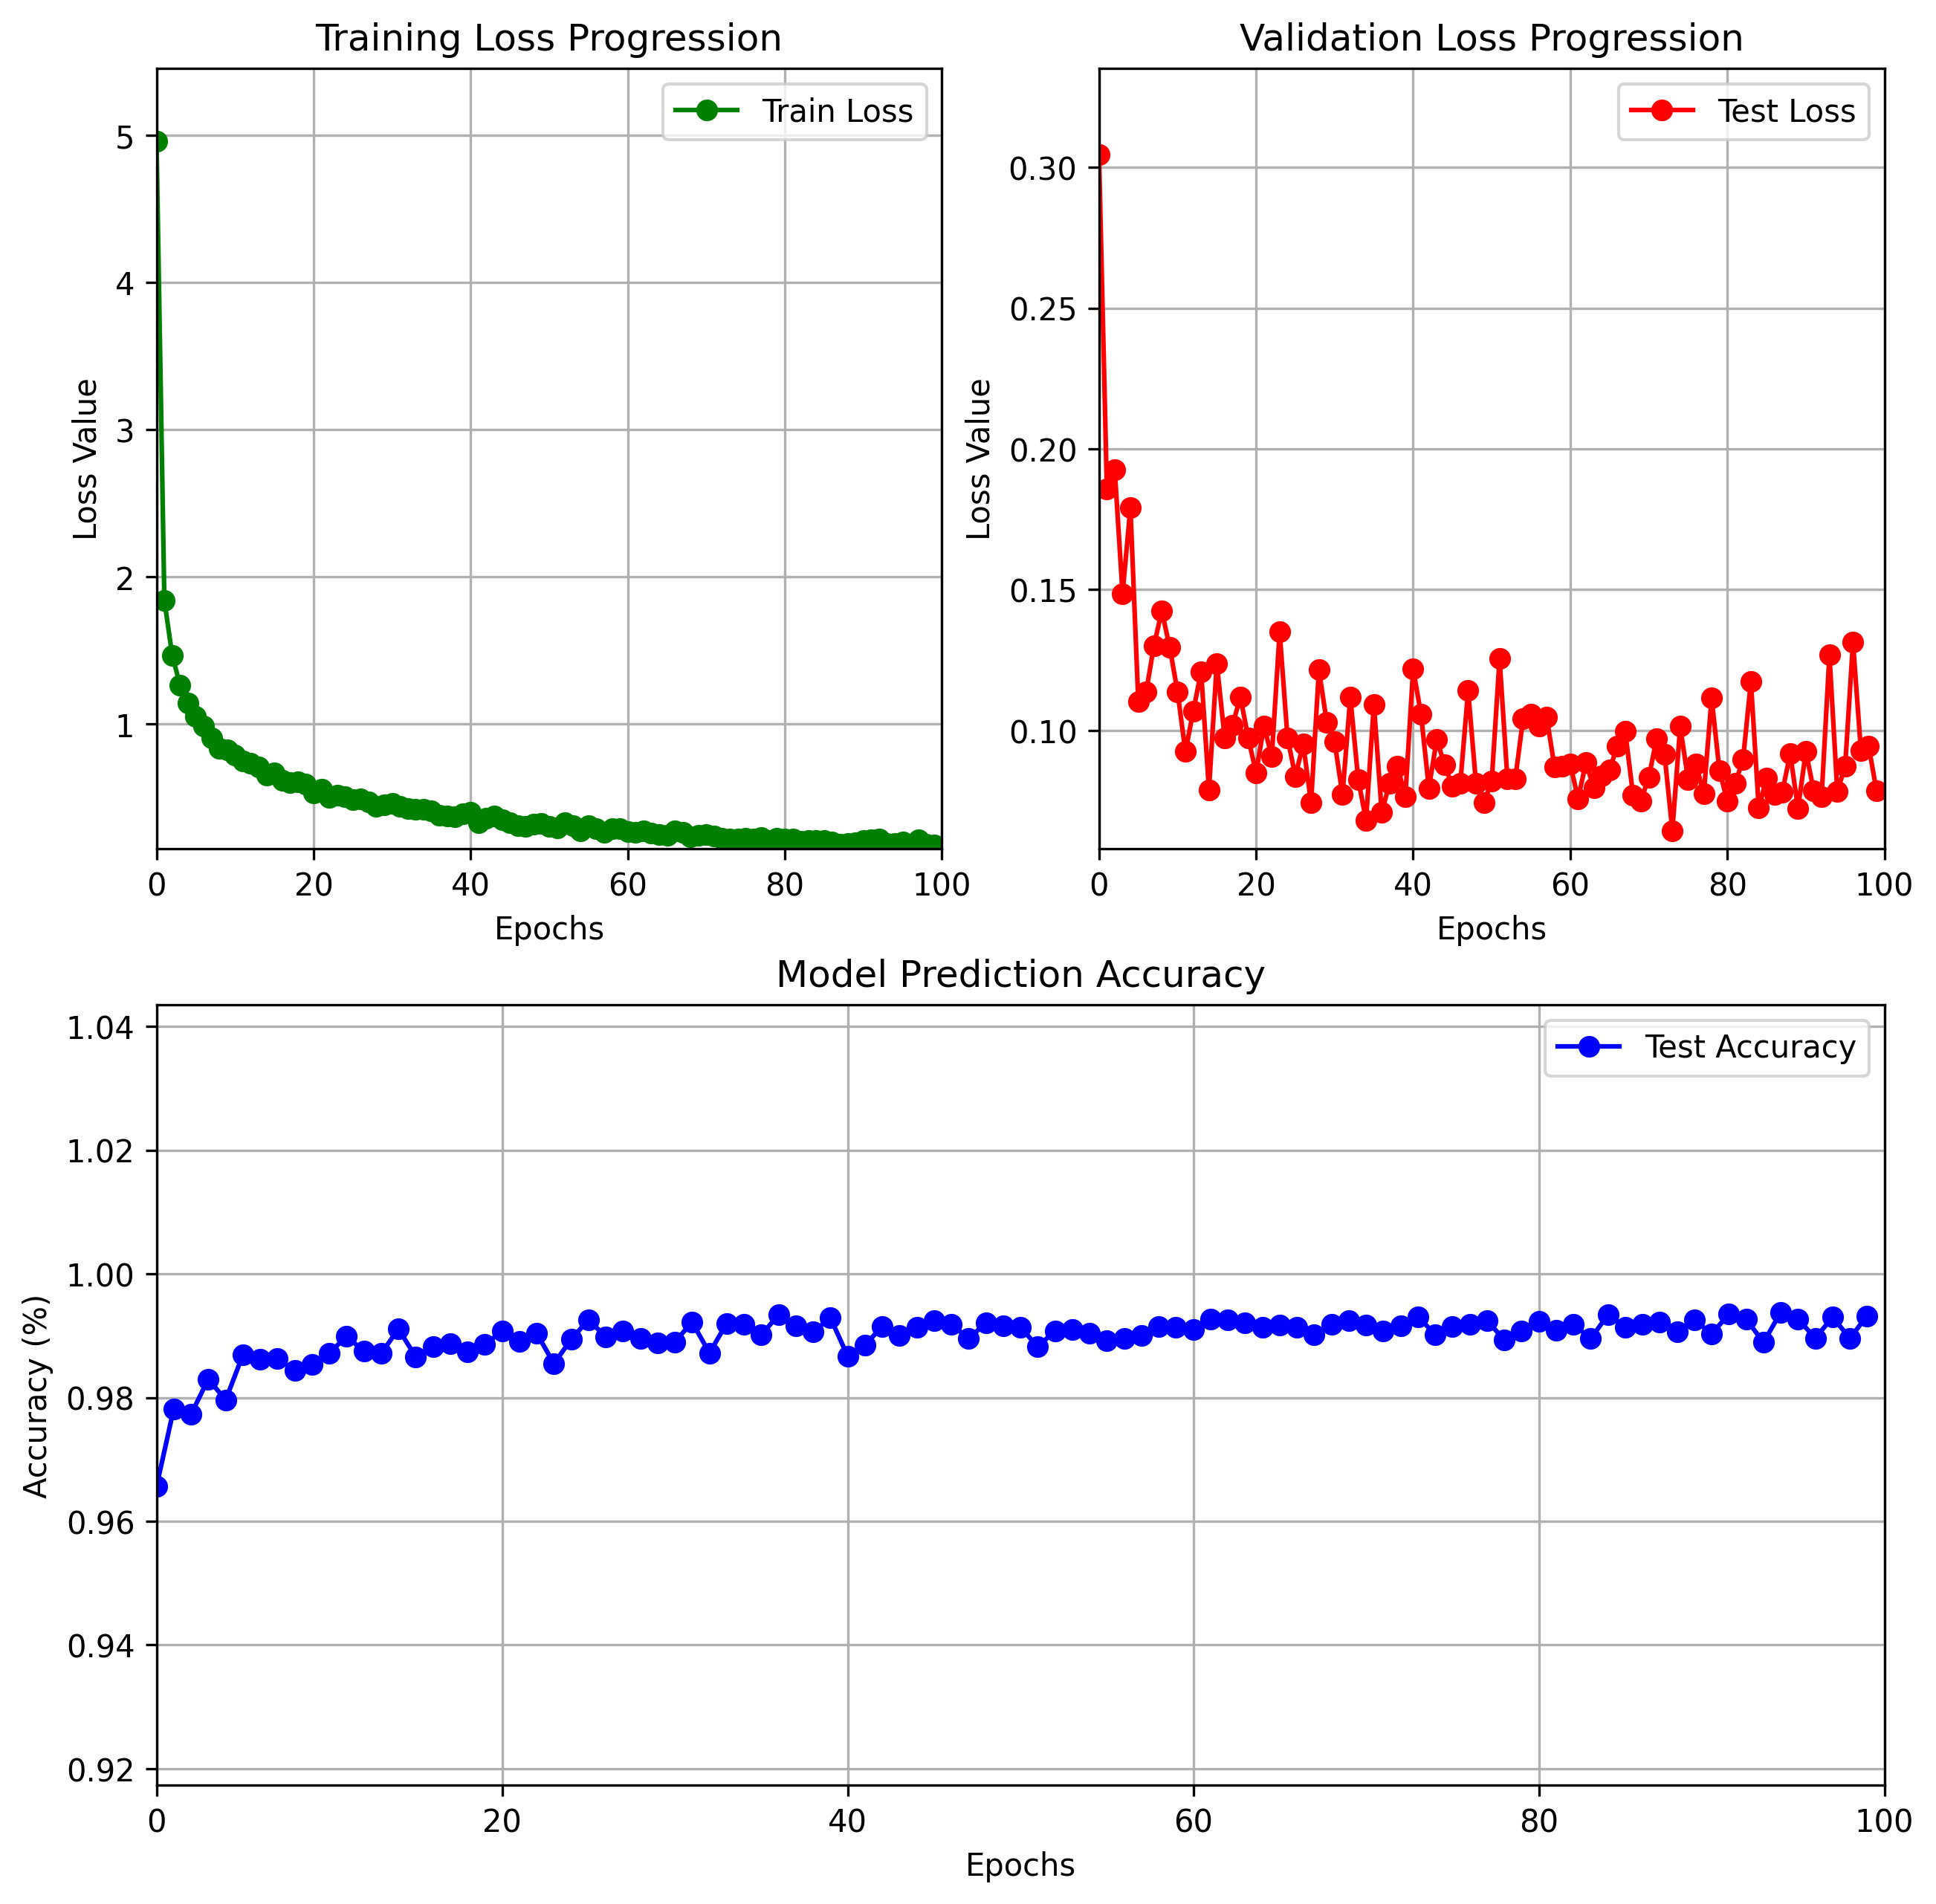
\includegraphics[width=0.45\textwidth]{fig/train_result_bsln_mnist.png} % 设定图片宽度
  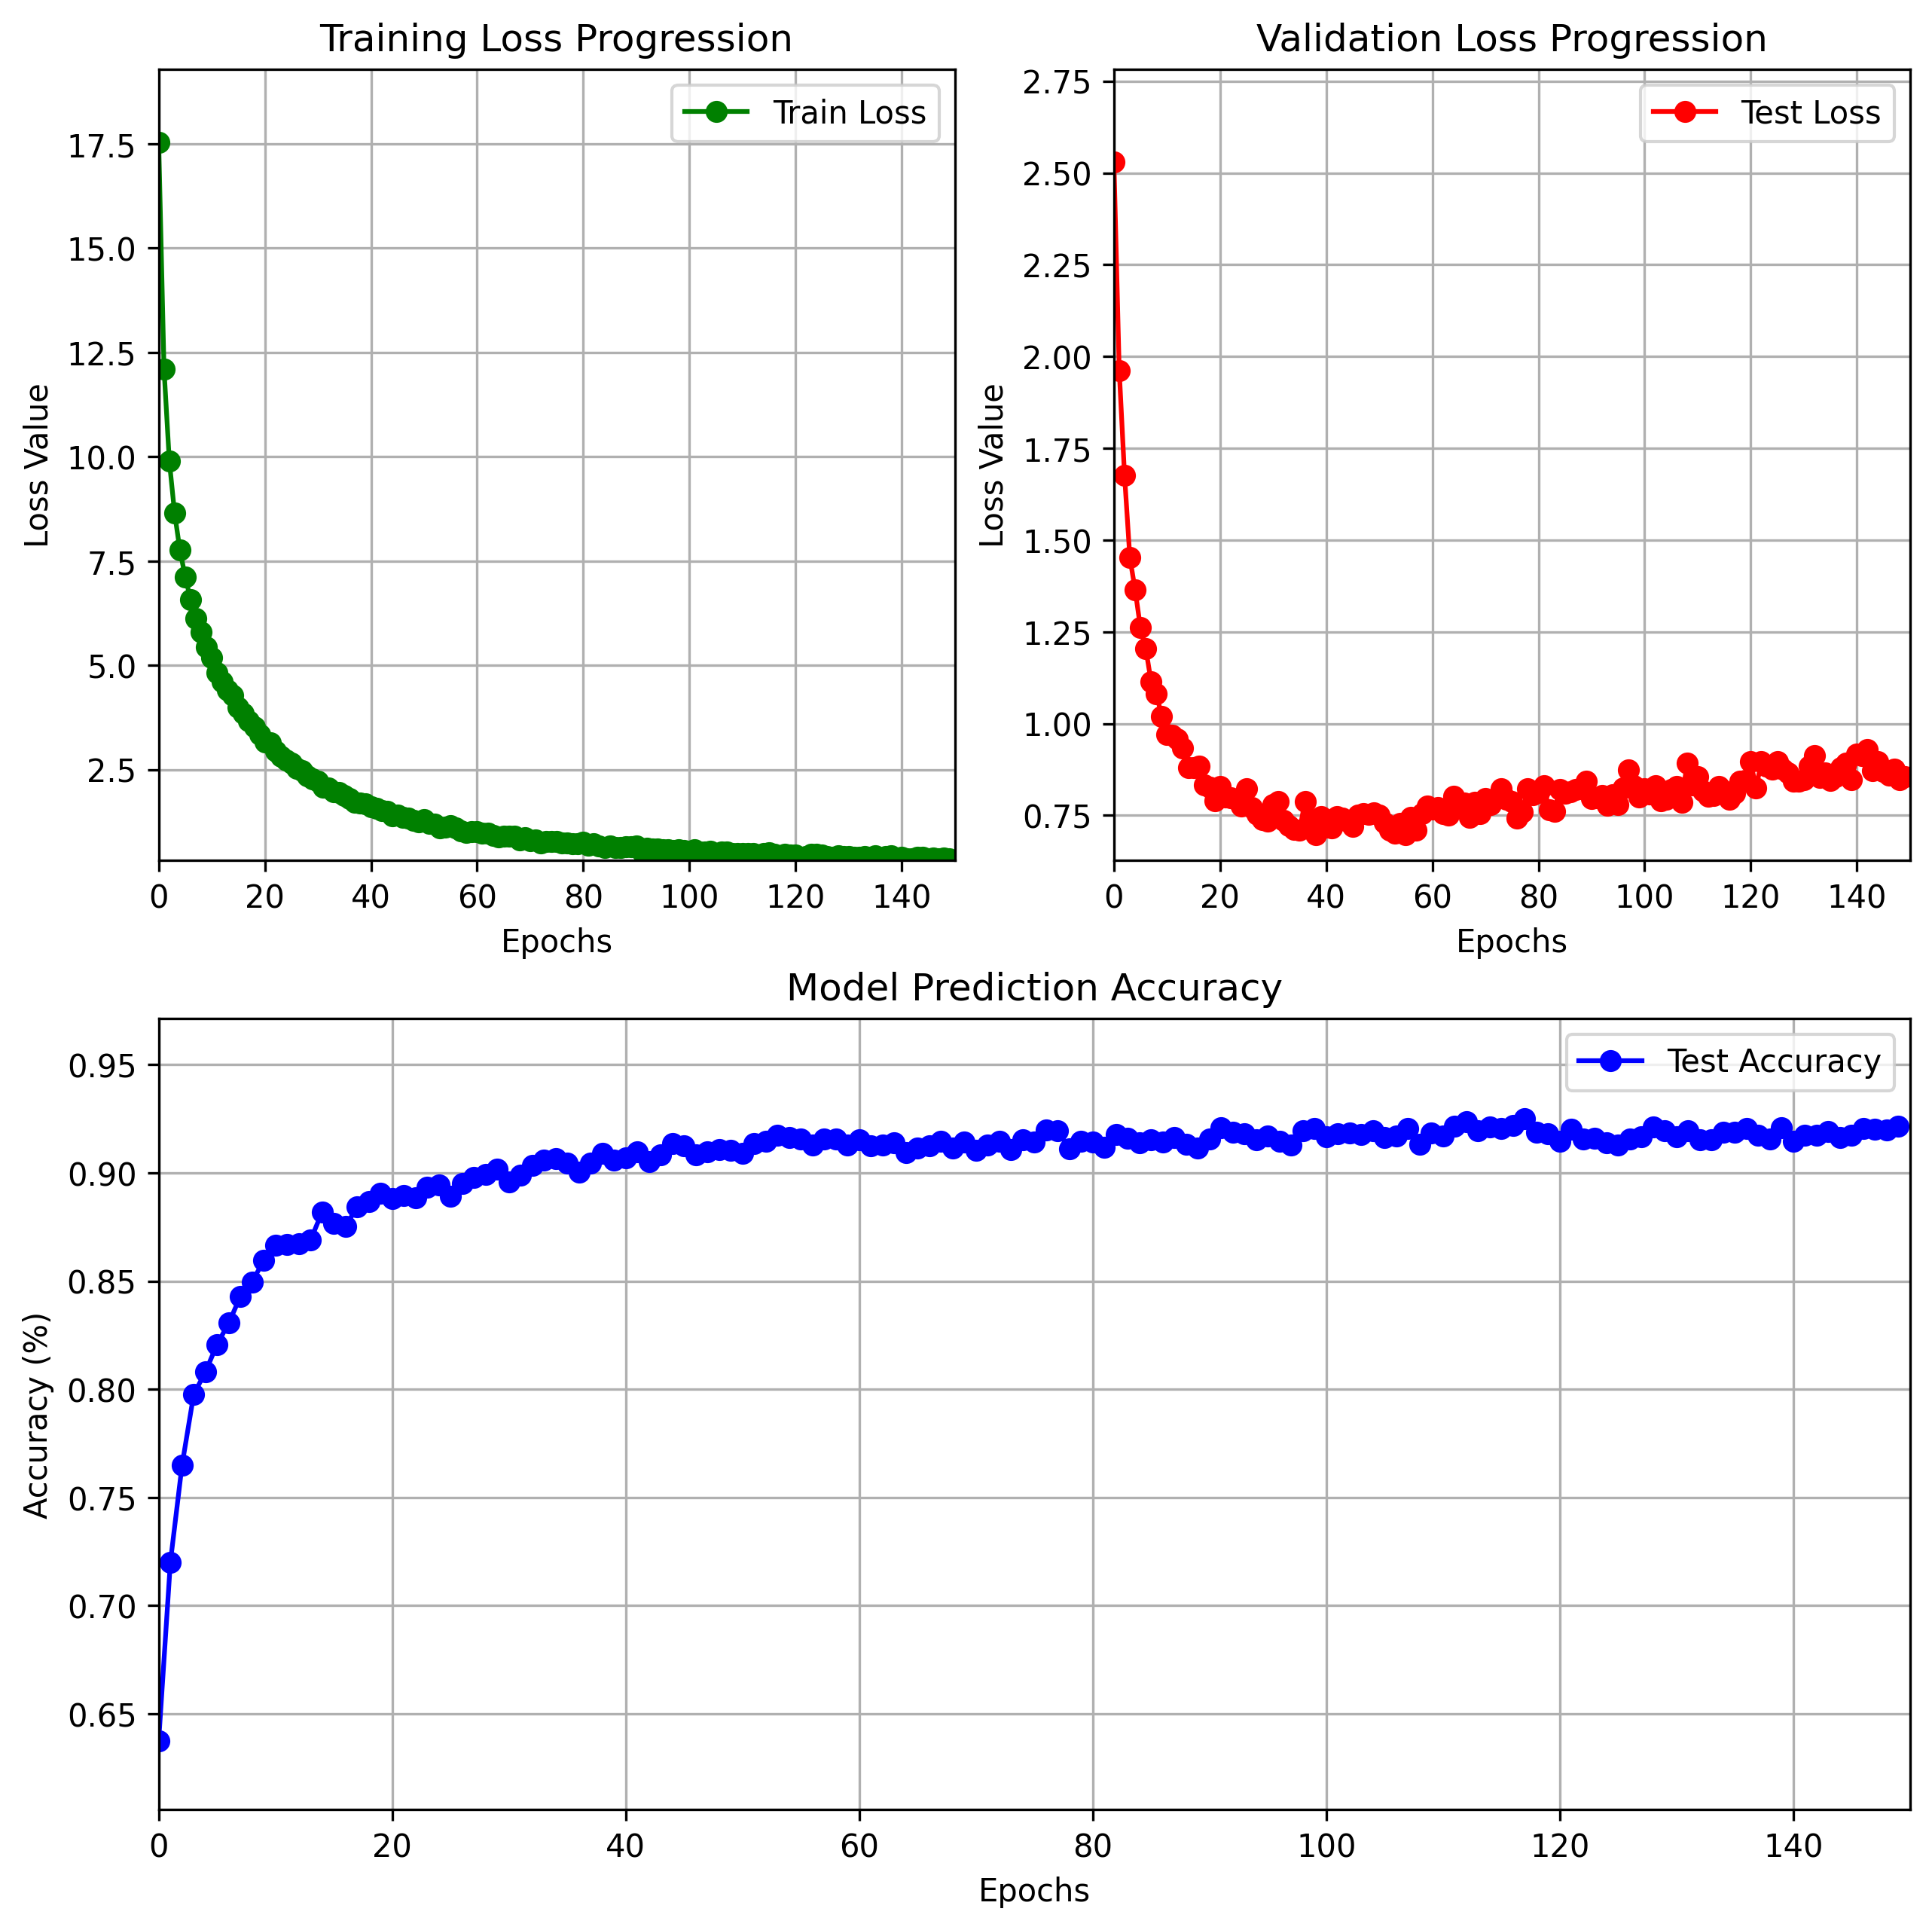
\includegraphics[width=0.45\textwidth]{fig/train_result_res18.png} % 设定图片宽度
  \caption{Basline(left), ResNet18(right) from Task A} % 图片标题
  \label{fig:curve} % 图片标签,方便引用
\end{figure}

\noindent\textbf{Conclusion}
we can see from Table 4. that the reproduced training and testing on MNIST of our self-made framework has converge to a fairly close testing accuracy: 98.9\%+ to that of Task A (torch).\\

However, see Figure 10 and Figure 11, the testing loss of our framewrok is more volitile that Task A, i think this might because:
\begin{itemize}
  \item Differences of default weights initialization: PyTorch's convolutional layers default to Kaiming Normal initialization, while my self-made one simply using \texttt{np.random.rand}
  \item Differences in hardware and parallelization algo: PyTorch may leverage more optimized cuDNN algorithms for convolutions, while our framework simply replace \texttt{numpy} with \texttt{cupy}
\end{itemize}


\secs{What have i learnt}
\noindent\textbf{From BackwardPropagation to AutoGrad}: In example code part-B we can learn how forward pass and backward pass work together in a neural network, but implementing backward pass is complicated and sometimes impossible (especially in complicated computation). Meanwhile we know that all computation in deep learning are basically consist of few basic functions like exponents, add, subtract, multiplication etc, so we can utilizie chain rule to calculate gradient no matter how complicated a computation might be. This is how AutoGrad comes into play, and this is the core of  all deep learning frameworks, including pytorch.\\

\noindent\textbf{Understand by creating}: During the process of building a framework, i learn extensively and experience moments of revelation like "ah, this is how a neural network works!" or "so this algorithm can be implemented this way!" These insights are unattainable through merely using existing tools like pytorch. Some concepts can only be understood by creating, some truths can only be seen by building. 

For instance, some may view deep learning frameworks as mere libraries pieced together with layers and functions. In reality, frameworks go far beyond that. A framework can be considered a programming language—specifically, one with automatic differentiation capabilities (recently termed a "differentiable programming language").
















% \secs{A4.1 (Implementing the Gradient Method)}
% We want to minimize the objective function
% \[
% \min_{x\in\mathbb{R}^2} f(x) = \frac{1}{2}x_1^4-x_1^3-x_1^2+x_1^2x_2^2+\frac{1}{2}x_2^4-x_2^2
% \]
% by gradient descent methods with different initial points and stepsize strategies, as presented in the following.\\

% \noindent Initial points: 
% \[
% \chi^0 := \left\{
% \begin{bmatrix}
% -\frac{1}{2} \\ 1
% \end{bmatrix},
% \begin{bmatrix}
% -\frac{1}{2} \\ \frac{1}{2}
% \end{bmatrix},
% \begin{bmatrix}
% -\frac{1}{4} \\ -\frac{1}{2}
% \end{bmatrix},
% \begin{bmatrix}
% \frac{1}{2} \\ -\frac{1}{2}
% \end{bmatrix},
% \begin{bmatrix}
% \frac{1}{2} \\ 1
% \end{bmatrix}
% \right\}
% \]
% \noindent stationary points of $f(x)$:
% \[
% \chi^* := \left\{
% \begin{bmatrix}
% 0 \\ 0
% \end{bmatrix},
% \begin{bmatrix}
% 2 \\ 0
% \end{bmatrix},
% \begin{bmatrix}
% -\frac{1}{2} \\ 0
% \end{bmatrix},
% \begin{bmatrix}
% 0 \\ 1
% \end{bmatrix},
% \begin{bmatrix}
% 0 \\ -1
% \end{bmatrix}
% \right\}
% \]



% %------------ backtracking--------------
% \subsection*{1. Backtracking}
% % \begingroup
% % \setlength{\intextsep}{0pt}%
% % \setlength{\columnsep}{0pt}%
% % \begin{wrapfigure}{r}{0.65\textwidth}%靠文字内容的右侧
% %   \centering
% %   \includegraphics[width=\linewidth]{Back Tracking.png}
% %   \caption{Backtracking Line Search}
% % \end{wrapfigure}

% Back Tracking line search: choose the largest $\alpha_k \in \{\sigma^k: k = 0,1,...\}$ that satisfies Armijo condition $f(x_k+\alpha_k d_k)-f(x_k)\leq \gamma \alpha_k \nabla f(x_k)^T d_k$ with $(\sigma, \gamma) = (0.5,0.1)$.\\
% \\
% Performance (in terms of iteration) of Backtracking Line Search stepsize strategy are shown below:\\
% \\
%   \begin{tabular}{ccc}
    
%     \hline
%     $x_0$ & iteration & limit point $x^*$\\
%     \hline
%           (-0.50,1.00) & 13 & (2.00,-0.00)  \\ % backtrack
%           (-0.50,0.50) & 325 & (-0.00,1.00) \\ % backtrack
%           (-0.25,-0.50) & 467 & (-0.00,-1.00)  \\ % backtrack
%           (0.50,-0.50) & 12 & (2.00,0.00)  \\ % backtrack
%           (0.50,1.00) & 10 & (2.00,-0.00)  \\ % backtrack
%           \hline
%           \multicolumn{3}{c}{Backtracking Line Search}\\
%           \hline
%   \end{tabular}

% %   \endgroup
% \newpage
% %------------------ exact line search ----------------------
% \subs{2. Exact Line Search}

% % \begingroup
% % \setlength{\intextsep}{0pt}%
% % \setlength{\columnsep}{0pt}%
% % \begin{wrapfigure}{r}{0.65\textwidth}%靠文字内容的右侧
% %   \centering
% %   \includegraphics[width=\linewidth]{Exact Line Search.png}
% %   %\caption{Exact Line Search}
% % \end{wrapfigure}

% Exact Line Search: aim at choosing the stepsize $\alpha_k$ that 
% \[
% \alpha_k = \underset{\alpha_k \geq 0}{argmin}\; f(x_k+\alpha_k d_k)
% \]
% Performance of Exact line search stepsize strategy are shown below:\\

% \noindent\begin{tabular}{ccc}
    
%   \hline
%   $x_0$ & iteration & limit point $x^*$\\
%   \hline
%   (-0.50,1.00) & 295 & (-0.00,1.00)   \\ % exactlineS
%   (-0.50,0.50) & 296 & (-0.00,1.00)  \\ % exactlineS
%   (-0.25,-0.50) & 375 & (-0.00,-1.00)  \\ % exactlineS
%   (0.50,-0.50) & 9 & (2.00,0.00) \\ % exactlineS
%   (0.50,1.00) & 6 & (2.00,0.00)  \\ % exactlineS
%         \hline
%         \multicolumn{3}{c}{Exact Line Search}\\
%         \hline
% \end{tabular}\\
% \\
% \textbf{\# PS}: the paths of 2 consecutive steps are not perpendicular because we constraint $\alpha_k \leq 1$ (because we search $\alpha$ in $[0,a]$, where $a=1$) insetead of not setting any constraint to them.

% % \endgroup
% \vspace{1cm}

% %------------- diminishing -----------------
% \subs{3. Diminishing Stepsize}

% % \begingroup
% % \setlength{\intextsep}{0pt}%
% % \setlength{\columnsep}{0pt}%
% % \begin{wrapfigure}{r}{0.65\textwidth}%靠文字内容的右侧
% %   \centering
% %   \includegraphics[width=\linewidth]{Diminishing Stepsize.png}
% %   %\caption{Diminishing Stepsize}
% % \end{wrapfigure}

% \noindent Diminishing Stepsize: we simply set
% \[
%   \alpha_k = \frac{1}{\sqrt{k+2}}
% \]
% where $k$ is the round of iteration.\\
% Performance of diminishing stepsize strategy are shown below:

% \noindent\begin{tabular}{ccc}
    
%   \hline
%   $x_0$ & iteration & limit point $x^*$\\
%   \hline
%   (-0.50,1.00) & 47 & (2.00,0.00)  \\ % diminishing
%   (-0.50,0.50) & 8523 & (-0.00,1.00) \\ % diminishing
%   (-0.25,-0.50) & 8501 & (-0.00,-1.00)  \\ % diminishing
%   (0.50,-0.50) & 47 & (2.00,-0.00)  \\ % diminishing
%   (0.50,1.00) & 47 & (2.00,0.00)  \\ % diminishing
%         \hline
%         \multicolumn{3}{c}{Diminishing Stepsize}\\
%         \hline
% \end{tabular}\\
% \\
% \textbf{\# PS}: Since HW sheet has no requirement on $k$, we follow the common sense that $k$ starts from 1, so the first stepsize is
% \[
%   \alpha_1 = \frac{1}{\sqrt{1+2}} = \frac{1}{\sqrt{3}} 
% \]

% % \endgroup

% \newpage
% %------------- conclusion of stepsize strategy ---------------
% Then we can conclude the performance of different stepsize strategies as the following table:

  % \begin{center}
  %   \begin{tabular}{|c|cccc|} 
  %       \hline
  %       Methods & $x_0$ & iteration & limit point $x^*$ & Global Minimum?\\
  %       \hline
  %       &(-0.50,1.00) & 13 & (2.00,-0.00) & yes\\ % backtrack
  %       &(-0.50,0.50) & 325 & (-0.00,1.00) & no \\ % backtrack
  %       Back Tracking&(-0.25,-0.50) & 467 & (-0.00,-1.00) & no \\ % backtrack
  %       &(0.50,-0.50) & 12 & (2.00,0.00) & yes \\ % backtrack
  %       &(0.50,1.00) & 10 & (2.00,-0.00) & yes \\ % backtrack
  %       \hline
      %   \hline
      %   &(-0.50,1.00) & 295 & (-0.00,1.00) & no \\ % exactlineS
      %   &(-0.50,0.50) & 296 & (-0.00,1.00) & no \\ % exactlineS
      %   Exact Line Search&(-0.25,-0.50) & 375 & (-0.00,-1.00) & no \\ % exactlineS
      %   &(0.50,-0.50) & 9 & (2.00,0.00) & yes \\ % exactlineS
      %   &(0.50,1.00) & 6 & (2.00,0.00) & yes \\ % exactlineS
      %   \hline
      %   \hline
      %   &(-0.50,1.00) & 47 & (2.00,0.00) & yes\\ % diminishing
      %   &(-0.50,0.50) & 8523 & (-0.00,1.00) & no \\ % diminishing
      %   Diminishing Stepsize&(-0.25,-0.50) & 8501 & (-0.00,-1.00) & no \\ % diminishing
      %   &(0.50,-0.50) & 47 & (2.00,-0.00) & yes\\ % diminishing
      %   &(0.50,1.00) & 47 & (2.00,0.00) & yes \\ % diminishing
      % \hline
%     \end{tabular} 
% \end{center}
% \newpage

% % \secs{A4.2 (Inertial Gradient Method)}

% % \noindent The convergence trace of gradient method with momentum of $\beta \in \{0.3,0.5,0.7,0.9\}$ and different initial points are shown below respectively:\\
% % \vspace{5mm}

% % \noindent\includegraphics[width=0.5\linewidth]{GD with momentum, beta=03.png}
% % \includegraphics[width=0.5\linewidth]{GD with momentum, beta=05.png}\\
% % \includegraphics[width=0.5\linewidth]{GD with momentum, beta=07.png}
% % \includegraphics[width=0.5\linewidth]{GD with momentum, beta=09.png}\\

% \subs{Performance Analysis}
% by comparing the average iteration numbers of GD with momentum and GD with different stepsize strategies (discussed in part A4.1):
% \begin{center}
%   \begin{tabular}{c|ccc|cccc}
%     \hline
%     \multicolumn{1}{c}{} & \multicolumn{3}{c}{Stepsize strategies} & \multicolumn{4}{c}{GD with momentum}\\
%     \hline
%     &Backtrack & Exact LineSearch & Diminishing & $\beta = 0.3$ & $\beta = 0.5$ & $\beta = 0.7$ & $\beta = 0.9$\\
%     \hline
%     Average Iteration & 164.5 & 196.2 & 3433.0 & 104.8& 51.8 & 90.2 & 1250.0\\
%     \hline
%     Probablity to Global Min & 0.6 & 0.4 & 0.6 & 0.8 & 1.0 & 1.0 &0.8\\
%     \hline
%   \end{tabular}
% \end{center}
% It is easy to see that \textbf{the average iteration (averaging across 5 different initial points) it takes to converge to some limit point is noticeably larger using stepsize strategies than GD with momentum in general.}  \\
% \\
% And we also notice GD with momentum converger faster when $\beta$ change from $0.3$ to $0.5$, then converger slower when $\beta$ goes from $0.5$ to $0.9$, how to interpretate this phenomenon? we can first look at the detail of how $\beta$ affect convergence: 

% \begin{center}
%   \begin{tabular}{|c|cccc|} 
%       \hline
%       $\beta$ & $x_0$ & iteration & limit point $x^*$ & Global Minimum? \\
%       \hline
%       &(-0.50,1.00) & 26 & (2.00,0.00) & yes\\ % momentum beta 0.3
%       &(-0.50,0.50) & 33 & (2.00,-0.00) & yes \\ % momentum beta 0.3
%       $\beta = 0.3$&\textcolor{red}{(-0.25,-0.50)} & \textcolor{red}{417} & \textcolor{red}{(-0.00,-1.00)} & no \\ % momentum beta 0.3
%       &(0.50,-0.50) & 24 & (2.00,0.00) & yes \\ % momentum beta 0.3
%       &(0.50,1.00) & 24 & (2.00,0.00) & yes \\ % momentum beta 0.3
%       \hline
%       \hline
%       &(-0.50,1.00) & 39 & (2.00,0.00) & yes \\ % momentum beta 0.5
%       &(-0.50,0.50) & 56 & (2.00,0.00) & yes \\ % momentum beta 0.5
%       $\beta = 0.5$&(-0.25,-0.50) & 88 & (2.00,0.00) & yes \\ % momentum beta 0.5
%       &(0.50,-0.50) & 37 & (2.00,-0.00) & yes \\ % momentum beta 0.5
%       &(0.50,1.00) & 39 & (2.00,0.00) & yes \\ % momentum beta 0.5
%       \hline
%       \hline
%       &(-0.50,1.00) & 105 & (2.00,0.00) & yes \\ % momentum beta 0.7
%       &(-0.50,0.50) & 88 & (2.00,0.00) & yes \\ % momentum beta 0.7
%       $\beta = 0.7$&(-0.25,-0.50) & 102 & (2.00,-0.00) & yes \\ % momentum beta 0.7
%       &(0.50,-0.50) & 77 & (2.00,-0.00) & yes \\ % momentum beta 0.7
%       &(0.50,1.00) & 79 & (2.00,-0.00) & yes \\ % momentum beta 0.7
%     \hline
%     \hline
%     &(-0.50,1.00) & 268 & (2.00,0.00) & yes \\ % momentum beta 0.9
%     &(-0.50,0.50)& 258 & (2.00,0.00) & yes \\ % momentum beta 0.9
%     $\beta = 0.9$&(-0.25,-0.50) & 276 & (2.00,0.00) & yes \\ % momentum beta 0.9
%     &(0.50,-0.50) & 297 & (2.00,-0.00) & yes \\ % momentum beta 0.9
%     &\textcolor{red}{(0.50,1.00)} & \textcolor{red}{5151} & \textcolor{red}{(-0.00,1.00)} & no \\ % momentum beta 0.9
%     \hline
%   \end{tabular} 
% \end{center}
% Notice when $\beta = 0.3$ and starting from the initial point $(-0.25,-0.5)$, GD converge to $(0,-1)$ while other initial points all converge to $(2,0)$, this is because the first several stepsize of GD heppen to be too large from this initial point and \textbf{pushing the trace to an area not ideal for fast convergence}, and by coincidence the trace finally converge to a different limit point from the other initial points, and the iterations it takes to converge go very high, this should \textbf{be treated as an anomoly.} Same with $\beta = 0.9$ initial point $(0.5,1.0)$: this very initial condition just happen to be not ideal for fast convergence.\\
% After dropping this anomoly we can get an averge iteration number of $26.75$ for $\beta = 0.3$, and the trend becomes obvious: $\beta$ smaller, converge faster. \\
% \\
% Another observation is that \textbf{GD with momentum is more likely to converge to the global minimum} $(2,0)$ than GD with stepsize strategies, this is also easy to explain: with "momentum" (brought by the momentum term $\beta (x_k-k_{k-1})$), the trace is more likely to "escape" from the local minimum.
% \newpage





\end{document}


